\documentclass[twoside]{book}

% Packages required by doxygen
\usepackage{calc}
\usepackage{doxygen}
\usepackage{graphicx}
\usepackage[utf8]{inputenc}
\usepackage{makeidx}
\usepackage{multicol}
\usepackage{multirow}
\usepackage{textcomp}
\usepackage[table]{xcolor}

% Font selection
\usepackage[T1]{fontenc}
\usepackage{mathptmx}
\usepackage[scaled=.90]{helvet}
\usepackage{courier}
\usepackage{amssymb}
\usepackage{sectsty}
\renewcommand{\familydefault}{\sfdefault}
\allsectionsfont{%
  \fontseries{bc}\selectfont%
  \color{darkgray}%
}
\renewcommand{\DoxyLabelFont}{%
  \fontseries{bc}\selectfont%
  \color{darkgray}%
}

% Page & text layout
\usepackage{geometry}
\geometry{%
  a4paper,%
  top=2.5cm,%
  bottom=2.5cm,%
  left=2.5cm,%
  right=2.5cm%
}
\tolerance=750
\hfuzz=15pt
\hbadness=750
\setlength{\emergencystretch}{15pt}
\setlength{\parindent}{0cm}
\setlength{\parskip}{0.2cm}
\makeatletter
\renewcommand{\paragraph}{%
  \@startsection{paragraph}{4}{0ex}{-1.0ex}{1.0ex}{%
    \normalfont\normalsize\bfseries\SS@parafont%
  }%
}
\renewcommand{\subparagraph}{%
  \@startsection{subparagraph}{5}{0ex}{-1.0ex}{1.0ex}{%
    \normalfont\normalsize\bfseries\SS@subparafont%
  }%
}
\makeatother

% Headers & footers
\usepackage{fancyhdr}
\pagestyle{fancyplain}
\fancyhead[LE]{\fancyplain{}{\bfseries\thepage}}
\fancyhead[CE]{\fancyplain{}{}}
\fancyhead[RE]{\fancyplain{}{\bfseries\leftmark}}
\fancyhead[LO]{\fancyplain{}{\bfseries\rightmark}}
\fancyhead[CO]{\fancyplain{}{}}
\fancyhead[RO]{\fancyplain{}{\bfseries\thepage}}
\fancyfoot[LE]{\fancyplain{}{}}
\fancyfoot[CE]{\fancyplain{}{}}
\fancyfoot[RE]{\fancyplain{}{\bfseries\scriptsize Generated on Tue Mar 10 2015 18\-:26\-:51 for Lagrangian Particle Code for The Simulation of 2\-D/3\-D Fluid Dynamics by Doxygen }}
\fancyfoot[LO]{\fancyplain{}{\bfseries\scriptsize Generated on Tue Mar 10 2015 18\-:26\-:51 for Lagrangian Particle Code for The Simulation of 2\-D/3\-D Fluid Dynamics by Doxygen }}
\fancyfoot[CO]{\fancyplain{}{}}
\fancyfoot[RO]{\fancyplain{}{}}
\renewcommand{\footrulewidth}{0.4pt}
\renewcommand{\chaptermark}[1]{%
  \markboth{#1}{}%
}
\renewcommand{\sectionmark}[1]{%
  \markright{\thesection\ #1}%
}

% Indices & bibliography
\usepackage{natbib}
\usepackage[titles]{tocloft}
\setcounter{tocdepth}{3}
\setcounter{secnumdepth}{5}
\makeindex

% Hyperlinks (required, but should be loaded last)
\usepackage{ifpdf}
\ifpdf
  \usepackage[pdftex,pagebackref=true]{hyperref}
\else
  \usepackage[ps2pdf,pagebackref=true]{hyperref}
\fi
\hypersetup{%
  colorlinks=true,%
  linkcolor=blue,%
  citecolor=blue,%
  unicode%
}

% Custom commands
\newcommand{\clearemptydoublepage}{%
  \newpage{\pagestyle{empty}\cleardoublepage}%
}


%===== C O N T E N T S =====

\begin{document}

% Titlepage & ToC
\hypersetup{pageanchor=false}
\pagenumbering{roman}
\begin{titlepage}
\vspace*{7cm}
\begin{center}%
{\Large Lagrangian Particle Code for The Simulation of 2\-D/3\-D Fluid Dynamics }\\
\vspace*{1cm}
{\large Generated by Doxygen 1.8.6}\\
\vspace*{0.5cm}
{\small Tue Mar 10 2015 18:26:51}\\
\end{center}
\end{titlepage}
\clearemptydoublepage
\tableofcontents
\clearemptydoublepage
\pagenumbering{arabic}
\hypersetup{pageanchor=true}

%--- Begin generated contents ---
\chapter{Main Page}
\label{index}\hypertarget{index}{}\hypertarget{index_sec1}{}\section{Overview of the Lagrangian Particle Method}\label{index_sec1}
A new Lagrangian particle method for solving Euler quations for compressible inviscid fluid or gas flows is developed by Hsinchiang Chen, Roman Samulyak, and Wei Li at the department of Applied Mathematics and Statistics at Stony Brook University. The preliminary results has been submitted to the Journal of Computational Physics (2015). Similar to Smoothed Particle Hydrodynamics (S\-P\-H) (see \href{http://en.wikipedia.org/wiki/Smoothed-particle_hydrodynamics}{\tt http\-://en.\-wikipedia.\-org/wiki/\-Smoothed-\/particle\-\_\-hydrodynamics} for S\-P\-H method), the method represents fluid cells with Lagrangian particles and is suitable for the simulation of complex free surface / multiphase flows. The main contributions of the proposed method, which is different from S\-P\-H in all other aspects, are\par
(a) Significant improvement of approximation of differential operators based on a polynomial fit and the corresponding weighted least squares problem and convergence of prescribed order\par
 (b) A new particle-\/based algorithm which provides both accuracy and long term stability\par
 (c) Elimination of the dependence on artificial parameters such as the smoothening length in S\-P\-H\par
 (d) Accurate resolution of states at free interfaces.\par
Numerical verification tests are performed and demonstrated the expected convergence order.\par
 \hypertarget{index_sec2}{}\section{Overview of the Lagrangian Particle Code}\label{index_sec2}
The Lagrangian Particle code implements the proposed Lagrangian Particle method and is capable of simulating both 2\-D and 3\-D fluid dynamics. Since 1\-D is of high research/experiment value we are merging a independent 1\-D code into this code now to make this code a full-\/fledged 1\-D/2\-D/3\-D fluid dynamics code. It is a C++ code which is parallelized using multithreads with the Open\-Mp A\-P\-Is. We have preliminary success on the speedups, which is about 5 times faster on 8 threads The most updated version of the code contains about 15 main modules, and about 35 modules in total, which contains over 10,000 lines of C/\-C++ code. There are currently two contributors to this code\-:\par
1). Hsinchiang Chen is the main author who design the code structure and implements almost all modules in this code\par
2). Kwangmin Yu is the second author who is intensively involved in the initial code struture design and internal data structure design. He is also the main author of the Neighbour\-Search and \hyperlink{classOctree}{Octree} classes.\par
 The accuracy of the proposed numerical algorithm and the code has been verified by comparing to results using M\-U\-S\-C\-L scheme with the Fron\-Tier code at the Stony Brook University. The results achieved the desired rate of convergence of the proposed algorithm.\par
 All test results on the accuracy, convergence, and parallel performance of the code will be updated soon.\hypertarget{index_sec3}{}\section{The Governing Equations}\label{index_sec3}
Consider the one-\/dimensional Lagrangian formulation of the Euler equations, written in the conservative form

\[ U_{t}^{'} + \left[ F(U^{'}) \right]_{x} = 0, \]

\[ U^{'} = \left( \begin{array} {c} V \\ u \\ E \end{array} \right), \, F(U^{'}) = V_{0} \left( \begin{array} {c} -u \\ P \\ Pu \end{array} \right), \]

where $V$ is the specific volume, $u$ is the velocity, $E$ is the specific total energy, and $P$ is the pressure.\par
 Further theories and derivations of equations of this method will be updated soon.\par
\hypertarget{index_sec4}{}\section{The Work Flow of the Code}\label{index_sec4}
We give a qualitative description of the code by using a flow chart describing how the algorithm/code works.

\hypertarget{index_sec5}{}\section{Simulation of 2\-D disks collision}\label{index_sec5}
The following simulation snapshots demonstrates the results of two 2\-D disks colliding with each other.

\hypertarget{index_sec6}{}\section{Simulation of 2\-D Gaussian-\/profile pressure propagation}\label{index_sec6}
The following simulation snapshots demonstrates the results of a 2\-D disk with a Gaussian-\/profile pressure initialization with the center of Gaussian being the center of the disk.



\begin{DoxyAuthor}{Author}
Chen, Hsin-\/\-Chiang (\href{mailto:morrischen2008@gmail.com}{\tt morrischen2008@gmail.\-com})
\end{DoxyAuthor}
Co-\/author\-: Yu, Kwangmin (\href{mailto:yukwangmin@gmail.com}{\tt yukwangmin@gmail.\-com})

\begin{DoxyVersion}{Version}
1.\-0
\end{DoxyVersion}
\begin{DoxyDate}{Date}
2015/03/09
\end{DoxyDate}
Created on\-: 2015/03/09 
\chapter{R\-E\-A\-D\-M\-E}
\label{md_README}
\hypertarget{md_README}{}
The Lagrangian Particle code for the simulation of fluid dynamics. Please see\-: hsinchiangchen.\-github.\-io/\-L\-P\-Fluid\-Code/index.html for documentation 
\chapter{Hierarchical Index}
\section{Class Hierarchy}
This inheritance list is sorted roughly, but not completely, alphabetically\-:\begin{DoxyCompactList}
\item \contentsline{section}{Bounding\-Box}{\pageref{classBoundingBox}}{}
\item \contentsline{section}{E\-O\-S}{\pageref{classEOS}}{}
\begin{DoxyCompactList}
\item \contentsline{section}{Polytropic\-Gas\-E\-O\-S}{\pageref{classPolytropicGasEOS}}{}
\item \contentsline{section}{Stiff\-Polytropic\-Gas\-E\-O\-S}{\pageref{classStiffPolytropicGasEOS}}{}
\end{DoxyCompactList}
\item \contentsline{section}{Geometry}{\pageref{classGeometry}}{}
\begin{DoxyCompactList}
\item \contentsline{section}{Ball}{\pageref{classBall}}{}
\item \contentsline{section}{Disk}{\pageref{classDisk}}{}
\item \contentsline{section}{Disk\-Left}{\pageref{classDiskLeft}}{}
\item \contentsline{section}{Disk\-Right}{\pageref{classDiskRight}}{}
\item \contentsline{section}{Line}{\pageref{classLine}}{}
\end{DoxyCompactList}
\item \contentsline{section}{Geometry\-Factory}{\pageref{classGeometryFactory}}{}
\item \contentsline{section}{Geometry\-Registrar$<$ Derived $>$}{\pageref{classGeometryRegistrar}}{}
\item \contentsline{section}{Hexagonal\-Packing2\-D}{\pageref{classHexagonalPacking2D}}{}
\item \contentsline{section}{Hexagonal\-Packing3\-D}{\pageref{classHexagonalPacking3D}}{}
\item \contentsline{section}{Initializer}{\pageref{classInitializer}}{}
\item \contentsline{section}{Key\-Index}{\pageref{structKeyIndex}}{}
\item \contentsline{section}{L\-P\-Solver}{\pageref{classLPSolver}}{}
\begin{DoxyCompactList}
\item \contentsline{section}{Hyperbolic\-L\-P\-Solver}{\pageref{classHyperbolicLPSolver}}{}
\item \contentsline{section}{Hyperbolic\-L\-P\-Solver1\-D}{\pageref{classHyperbolicLPSolver1D}}{}
\end{DoxyCompactList}
\item \contentsline{section}{L\-S\-Solver}{\pageref{classLSSolver}}{}
\begin{DoxyCompactList}
\item \contentsline{section}{Q\-R\-Solver}{\pageref{classQRSolver}}{}
\end{DoxyCompactList}
\item \contentsline{section}{Neighbour\-Searcher}{\pageref{classNeighbourSearcher}}{}
\begin{DoxyCompactList}
\item \contentsline{section}{Octree\-Searcher}{\pageref{classOctreeSearcher}}{}
\end{DoxyCompactList}
\item \contentsline{section}{Octree}{\pageref{classOctree}}{}
\item \contentsline{section}{Particle\-Data}{\pageref{classParticleData}}{}
\item \contentsline{section}{Particle\-Viewer}{\pageref{classParticleViewer}}{}
\begin{DoxyCompactList}
\item \contentsline{section}{T\-X\-T\-Particle\-Viewer1\-D}{\pageref{classTXTParticleViewer1D}}{}
\item \contentsline{section}{V\-T\-K\-Particle\-Viewer}{\pageref{classVTKParticleViewer}}{}
\end{DoxyCompactList}
\item \contentsline{section}{Search\-Result}{\pageref{structSearchResult}}{}
\item \contentsline{section}{State}{\pageref{classState}}{}
\begin{DoxyCompactList}
\item \contentsline{section}{Gaussian\-Pressure1\-D\-State}{\pageref{classGaussianPressure1DState}}{}
\item \contentsline{section}{Gaussian\-Pressure\-State}{\pageref{classGaussianPressureState}}{}
\item \contentsline{section}{Left\-Uniform\-Velocity\-State}{\pageref{classLeftUniformVelocityState}}{}
\item \contentsline{section}{Right\-Uniform\-Velocity\-State}{\pageref{classRightUniformVelocityState}}{}
\item \contentsline{section}{Uniform\-Velocity\-State}{\pageref{classUniformVelocityState}}{}
\end{DoxyCompactList}
\item \contentsline{section}{State\-Factory}{\pageref{classStateFactory}}{}
\item \contentsline{section}{State\-Registrar$<$ Derived $>$}{\pageref{classStateRegistrar}}{}
\item \contentsline{section}{Time\-Controller}{\pageref{classTimeController}}{}
\begin{DoxyCompactList}
\item \contentsline{section}{Default\-Time\-Controller}{\pageref{classDefaultTimeController}}{}
\end{DoxyCompactList}
\end{DoxyCompactList}

\chapter{Class Index}
\section{Class List}
Here are the classes, structs, unions and interfaces with brief descriptions\-:\begin{DoxyCompactList}
\item\contentsline{section}{\hyperlink{classBall}{Ball} \\*Supply functions for generating a 3\-D ball geometry }{\pageref{classBall}}{}
\item\contentsline{section}{\hyperlink{classBoundingBox}{Bounding\-Box} \\*This class is keeps the information of the boundaries of a fluid/boundary object }{\pageref{classBoundingBox}}{}
\item\contentsline{section}{\hyperlink{classDefaultTimeController}{Default\-Time\-Controller} \\*This time controller calculates the time stepping based on the C\-F\-L condition }{\pageref{classDefaultTimeController}}{}
\item\contentsline{section}{\hyperlink{classDisk}{Disk} \\*Supply functions for generating a 2\-D disk geometry }{\pageref{classDisk}}{}
\item\contentsline{section}{\hyperlink{classDiskLeft}{Disk\-Left} \\*Supply functions for generating a 2\-D disk geometry for the 2\-D collision simulation }{\pageref{classDiskLeft}}{}
\item\contentsline{section}{\hyperlink{classDiskRight}{Disk\-Right} \\*Supply functions for generating a 2\-D disk geometry for the 2\-D collision simulation }{\pageref{classDiskRight}}{}
\item\contentsline{section}{\hyperlink{classEOS}{E\-O\-S} \\*An abstract class for the calculation of energy and sound speed based on different \hyperlink{classEOS}{E\-O\-S} models }{\pageref{classEOS}}{}
\item\contentsline{section}{\hyperlink{classGaussianPressureState}{Gaussian\-Pressure\-State} \\*A class that implements the Gaussian pressure state }{\pageref{classGaussianPressureState}}{}
\item\contentsline{section}{\hyperlink{classGeometry}{Geometry} \\*An abstract class for the initialization of the geometry of fluid objects }{\pageref{classGeometry}}{}
\item\contentsline{section}{\hyperlink{classGeometryFactory}{Geometry\-Factory} \\*The abstract factory class for creating objects in the \hyperlink{classGeometry}{Geometry} family }{\pageref{classGeometryFactory}}{}
\item\contentsline{section}{\hyperlink{classGeometryRegistrar}{Geometry\-Registrar$<$ Derived $>$} \\*A template class for the registration of classes in the \hyperlink{classGeometry}{Geometry} family }{\pageref{classGeometryRegistrar}}{}
\item\contentsline{section}{\hyperlink{classHexagonalPacking2D}{Hexagonal\-Packing2\-D} \\*Computes the 2\-D Cartesian coordinates of a particle based on the hexagonal close packing }{\pageref{classHexagonalPacking2D}}{}
\item\contentsline{section}{\hyperlink{classHexagonalPacking3D}{Hexagonal\-Packing3\-D} \\*Computes the 3\-D Cartesian coordinates of a particle based on the hexagonal close packing }{\pageref{classHexagonalPacking3D}}{}
\item\contentsline{section}{\hyperlink{classHyperbolicLPSolver}{Hyperbolic\-L\-P\-Solver} \\*The default Lagrangian Particle solver for the compressible Euler's equation }{\pageref{classHyperbolicLPSolver}}{}
\item\contentsline{section}{\hyperlink{classInitializer}{Initializer} \\*This class initializes the simulation }{\pageref{classInitializer}}{}
\item\contentsline{section}{\hyperlink{structKeyIndex}{Key\-Index} \\*This struct contains the morton key and the index of a particle. a vector of such structs is then sorted by the \char`\"{}key\char`\"{} field }{\pageref{structKeyIndex}}{}
\item\contentsline{section}{\hyperlink{classLeftUniformVelocityState}{Left\-Uniform\-Velocity\-State} \\*A class that implements the left uniform velocity state }{\pageref{classLeftUniformVelocityState}}{}
\item\contentsline{section}{\hyperlink{classLPSolver}{L\-P\-Solver} \\*An abstract class for the family of Lagrangian Particle solvers }{\pageref{classLPSolver}}{}
\item\contentsline{section}{\hyperlink{classLSSolver}{L\-S\-Solver} \\*An abstract class for the family of solvers for the least squares problem }{\pageref{classLSSolver}}{}
\item\contentsline{section}{\hyperlink{classNeighbourSearcher}{Neighbour\-Searcher} \\*An abstract class for the family of classes that performs the task of nearest neighbour search for particles }{\pageref{classNeighbourSearcher}}{}
\item\contentsline{section}{\hyperlink{classOctree}{Octree} \\*This class contains the \hyperlink{classOctree}{Octree} data structure and algorithm for nearest neighbour search of particles }{\pageref{classOctree}}{}
\item\contentsline{section}{\hyperlink{classOctreeSearcher}{Octree\-Searcher} \\*A class that searches nearest neighbours of particles based on the \hyperlink{classOctree}{Octree} data structure and algorithm }{\pageref{classOctreeSearcher}}{}
\item\contentsline{section}{\hyperlink{classParticleData}{Particle\-Data} \\*A class that stores all information and data of particles, such as x, y, and z coordinates, neighbour lists, and bounding boxes }{\pageref{classParticleData}}{}
\item\contentsline{section}{\hyperlink{classParticleViewer}{Particle\-Viewer} \\*An abstract class for classes that output simulations results }{\pageref{classParticleViewer}}{}
\item\contentsline{section}{\hyperlink{classPolytropicGasEOS}{Polytropic\-Gas\-E\-O\-S} \\*Calculates energy and sound speed based on the Polytropic gas eos model }{\pageref{classPolytropicGasEOS}}{}
\item\contentsline{section}{\hyperlink{classQRSolver}{Q\-R\-Solver} \\*A class which solves the least squares problem by the Q\-R decomposition method }{\pageref{classQRSolver}}{}
\item\contentsline{section}{\hyperlink{classRightUniformVelocityState}{Right\-Uniform\-Velocity\-State} \\*A class that implements the right uniform velocity state }{\pageref{classRightUniformVelocityState}}{}
\item\contentsline{section}{\hyperlink{structSearchResult}{Search\-Result} \\*A simple struct for the neighbour search result }{\pageref{structSearchResult}}{}
\item\contentsline{section}{\hyperlink{classState}{State} \\*An abstract class for the initialization of the state of fluid objects }{\pageref{classState}}{}
\item\contentsline{section}{\hyperlink{classStateFactory}{State\-Factory} \\*The abstract factory class for creating objects in the \hyperlink{classState}{State} family }{\pageref{classStateFactory}}{}
\item\contentsline{section}{\hyperlink{classStateRegistrar}{State\-Registrar$<$ Derived $>$} \\*A template class for the registration of classes in the \hyperlink{classState}{State} family }{\pageref{classStateRegistrar}}{}
\item\contentsline{section}{\hyperlink{classStiffPolytropicGasEOS}{Stiff\-Polytropic\-Gas\-E\-O\-S} \\*Calculates energy and sound speed based on the Stiffened Polytropic gas eos model }{\pageref{classStiffPolytropicGasEOS}}{}
\item\contentsline{section}{\hyperlink{classTimeController}{Time\-Controller} \\*An abstract class for different types of simulation time controllers }{\pageref{classTimeController}}{}
\item\contentsline{section}{\hyperlink{classUniformVelocityState}{Uniform\-Velocity\-State} \\*A class that implements the uniform velocity state }{\pageref{classUniformVelocityState}}{}
\item\contentsline{section}{\hyperlink{classVTKParticleViewer}{V\-T\-K\-Particle\-Viewer} \\*A class that output simulations results in the .vtk format }{\pageref{classVTKParticleViewer}}{}
\end{DoxyCompactList}

\chapter{File Index}
\section{File List}
Here is a list of all documented files with brief descriptions\-:\begin{DoxyCompactList}
\item\contentsline{section}{\hyperlink{eos_8h}{eos.\-h} \\*This header file contains classes for the calculation of the Equation of \hyperlink{classState}{State} (\hyperlink{classEOS}{E\-O\-S}) }{\pageref{eos_8h}}{}
\item\contentsline{section}{\hyperlink{geometry_8h}{geometry.\-h} \\*This header file contains classes for the initialization of the geometry of fluid objects }{\pageref{geometry_8h}}{}
\item\contentsline{section}{\hyperlink{geometry__collision_8h}{geometry\-\_\-collision.\-h} \\*This header file contains classes for the initialization of the geometry of fluid objects in the collision simulation }{\pageref{geometry__collision_8h}}{}
\item\contentsline{section}{\hyperlink{hexagonal__packing_8h}{hexagonal\-\_\-packing.\-h} \\*This header file contains classes for creating particles based on the 2\-D and 3\-D hexagonal close packing }{\pageref{hexagonal__packing_8h}}{}
\item\contentsline{section}{\hyperlink{initializer_8h}{initializer.\-h} \\*This header file contains classes for the initialization of the simulation }{\pageref{initializer_8h}}{}
\item\contentsline{section}{\hyperlink{lp__solver_8h}{lp\-\_\-solver.\-h} \\*This header file contains classes of the main Lagrangian Particle solvers such as the hyperbolic solvers and the elliptic solvers }{\pageref{lp__solver_8h}}{}
\item\contentsline{section}{\hyperlink{ls__solver_8h}{ls\-\_\-solver.\-h} \\*This header file contains classes for solvers of the least squares problem Ax = b }{\pageref{ls__solver_8h}}{}
\item\contentsline{section}{\hyperlink{neighbour__searcher_8h}{neighbour\-\_\-searcher.\-h} \\*This header file contains classes for searching nearest neighbours of particles using different algorithms such as octrees }{\pageref{neighbour__searcher_8h}}{}
\item\contentsline{section}{\hyperlink{octree_8h}{octree.\-h} \\*This header file contains classes for the \hyperlink{classOctree}{Octree} data structure and nearest neighbour search algorithms }{\pageref{octree_8h}}{}
\item\contentsline{section}{\hyperlink{particle__data_8h}{particle\-\_\-data.\-h} \\*This header file contains classes for storing information and data of particles, such as x, y, and z coordinates, neighbour lists, and bounding boxes }{\pageref{particle__data_8h}}{}
\item\contentsline{section}{\hyperlink{particle__viewer_8h}{particle\-\_\-viewer.\-h} \\*This header file contains classes for output simulation results in various formats such as .vtk }{\pageref{particle__viewer_8h}}{}
\item\contentsline{section}{\hyperlink{registrar_8h}{registrar.\-h} \\*This header file contains template registrar classes for the \hyperlink{classGeometry}{Geometry} and \hyperlink{classState}{State} family }{\pageref{registrar_8h}}{}
\item\contentsline{section}{\hyperlink{state_8h}{state.\-h} \\*This header file contains classes for the initialization of the state of fluid objects }{\pageref{state_8h}}{}
\item\contentsline{section}{\hyperlink{state__collision_8h}{state\-\_\-collision.\-h} \\*This header file contains classes for the initialization of the state of fluid objects in the 2\-D collision simulation }{\pageref{state__collision_8h}}{}
\item\contentsline{section}{\hyperlink{time__controller_8h}{time\-\_\-controller.\-h} \\*This header file contains classes for simulation time controls }{\pageref{time__controller_8h}}{}
\end{DoxyCompactList}

\chapter{Class Documentation}
\hypertarget{classBall}{\section{Ball Class Reference}
\label{classBall}\index{Ball@{Ball}}
}


Supply functions for generating a 3\-D ball geometry.  




{\ttfamily \#include $<$geometry.\-h$>$}

Inheritance diagram for Ball\-:\begin{figure}[H]
\begin{center}
\leavevmode
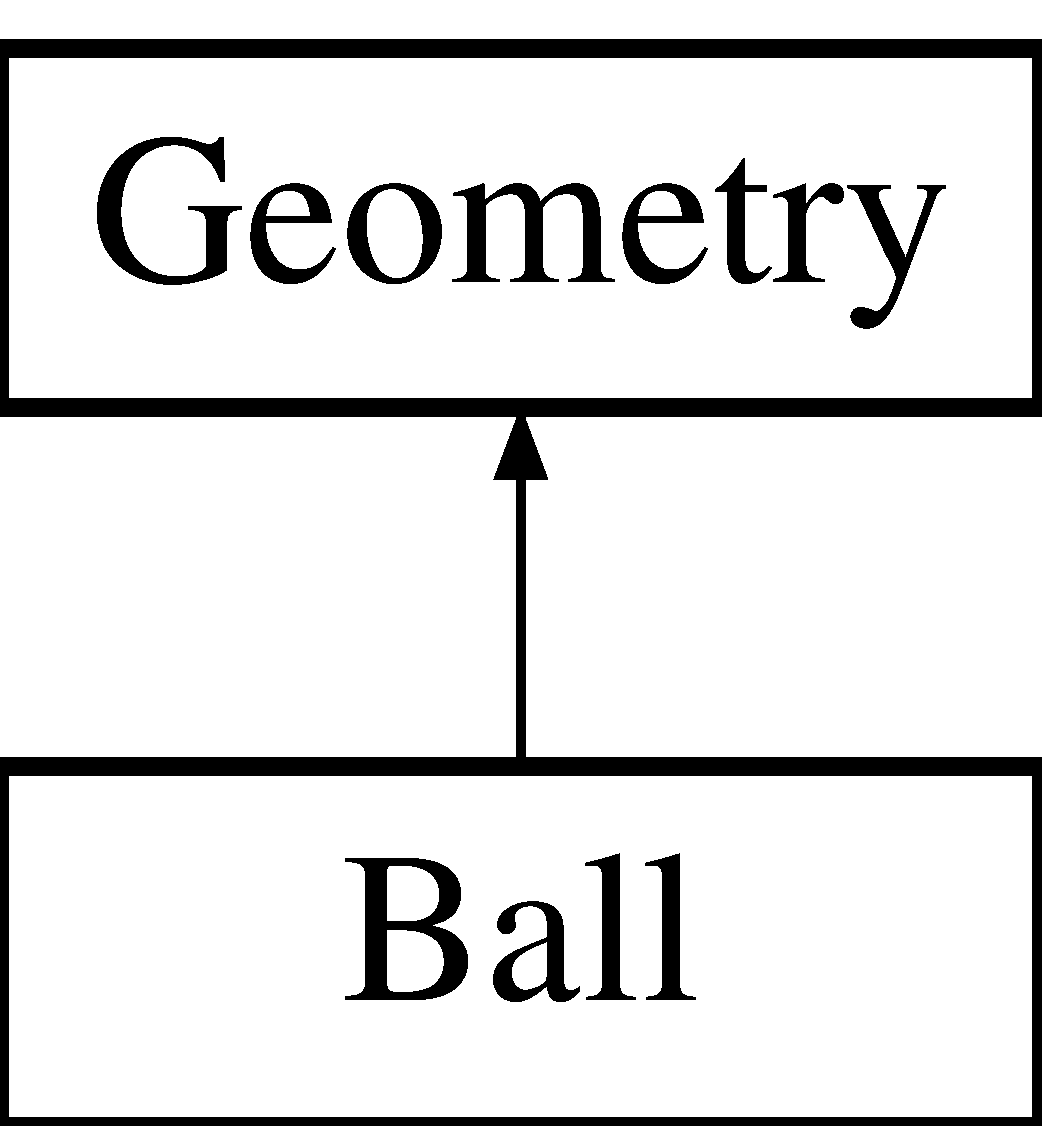
\includegraphics[height=2.000000cm]{classBall}
\end{center}
\end{figure}
\subsection*{Public Member Functions}
\begin{DoxyCompactItemize}
\item 
\hypertarget{classBall_a86a144d3dad6c953e422e32435923bbb}{\hyperlink{classBall_a86a144d3dad6c953e422e32435923bbb}{Ball} ()}\label{classBall_a86a144d3dad6c953e422e32435923bbb}

\begin{DoxyCompactList}\small\item\em Constructor. \end{DoxyCompactList}\item 
\hypertarget{classBall_a78aa1f06b39fc9f81df82bef399c475c}{virtual \hyperlink{classBall_a78aa1f06b39fc9f81df82bef399c475c}{$\sim$\-Ball} ()}\label{classBall_a78aa1f06b39fc9f81df82bef399c475c}

\begin{DoxyCompactList}\small\item\em Destructor. \end{DoxyCompactList}\item 
virtual bool \hyperlink{classBall_a3768880c8851caa9125b967c1083043c}{operator()} (double x, double y, double z) const 
\begin{DoxyCompactList}\small\item\em Level set function of a 3\-D ball. \end{DoxyCompactList}\item 
virtual void \hyperlink{classBall_ad9768e543e28ba727488f51eb80dc35a}{get\-Bounding\-Box} (double \&xmin, double \&xmax, double \&ymin, double \&ymax, double \&zmin, double \&zmax)
\begin{DoxyCompactList}\small\item\em Calculates the bounding box of 3\-D ball. \end{DoxyCompactList}\end{DoxyCompactItemize}


\subsection{Detailed Description}
Supply functions for generating a 3\-D ball geometry. 

\begin{DoxyAuthor}{Author}
Chen, Hsin-\/\-Chiang (\href{mailto:morrischen2008@gmail.com}{\tt morrischen2008@gmail.\-com})
\end{DoxyAuthor}
\begin{DoxyVersion}{Version}
1.\-0
\end{DoxyVersion}
\begin{DoxyDate}{Date}
2014/08/08
\end{DoxyDate}
Created on\-: 2014/06/07 

\subsection{Member Function Documentation}
\hypertarget{classBall_ad9768e543e28ba727488f51eb80dc35a}{\index{Ball@{Ball}!get\-Bounding\-Box@{get\-Bounding\-Box}}
\index{get\-Bounding\-Box@{get\-Bounding\-Box}!Ball@{Ball}}
\subsubsection[{get\-Bounding\-Box}]{\setlength{\rightskip}{0pt plus 5cm}void Ball\-::get\-Bounding\-Box (
\begin{DoxyParamCaption}
\item[{double \&}]{xmin, }
\item[{double \&}]{xmax, }
\item[{double \&}]{ymin, }
\item[{double \&}]{ymax, }
\item[{double \&}]{zmin, }
\item[{double \&}]{zmax}
\end{DoxyParamCaption}
)\hspace{0.3cm}{\ttfamily [virtual]}}}\label{classBall_ad9768e543e28ba727488f51eb80dc35a}


Calculates the bounding box of 3\-D ball. 


\begin{DoxyParams}[1]{Parameters}
\mbox{\tt out}  & {\em xmin} & The minimum in x-\/coordinate \\
\hline
\mbox{\tt out}  & {\em xmax} & The maximum in x-\/coordinate \\
\hline
\mbox{\tt out}  & {\em ymin} & The minimum in y-\/coordinate \\
\hline
\mbox{\tt out}  & {\em ymax} & The maximum in y-\/coordinate \\
\hline
\mbox{\tt out}  & {\em zmin} & The minimum in z-\/coordinate \\
\hline
\mbox{\tt out}  & {\em zmax} & The maximum in z-\/coordinate \\
\hline
\end{DoxyParams}
\begin{DoxyReturn}{Returns}
None 
\end{DoxyReturn}


Implements \hyperlink{classGeometry_aa8c0f7ecf1cfb99c4f997399ffe3fdb7}{Geometry}.

\hypertarget{classBall_a3768880c8851caa9125b967c1083043c}{\index{Ball@{Ball}!operator()@{operator()}}
\index{operator()@{operator()}!Ball@{Ball}}
\subsubsection[{operator()}]{\setlength{\rightskip}{0pt plus 5cm}bool Ball\-::operator() (
\begin{DoxyParamCaption}
\item[{double}]{x, }
\item[{double}]{y, }
\item[{double}]{z}
\end{DoxyParamCaption}
) const\hspace{0.3cm}{\ttfamily [virtual]}}}\label{classBall_a3768880c8851caa9125b967c1083043c}


Level set function of a 3\-D ball. 

The level set function is $ (x-\mbox{xcen})^2+(y-\mbox{ycen})^2+(z-\mbox{zcen})^2 \leq r^2 $ , where (xcen,ycen,zcen) and {\itshape r} refer to the center and the radius of the ball


\begin{DoxyParams}[1]{Parameters}
\mbox{\tt in}  & {\em x} & The x-\/coordinate \\
\hline
\mbox{\tt in}  & {\em y} & The y-\/coordinate \\
\hline
\mbox{\tt in}  & {\em z} & The z-\/coordinate \\
\hline
\end{DoxyParams}
\begin{DoxyReturn}{Returns}
{\ttfamily true} if (x,y,z) is inside the level set function; {\ttfamily false} otherwise 
\end{DoxyReturn}


Implements \hyperlink{classGeometry_a69dbaf841341db31d0c412bcdbf50766}{Geometry}.



The documentation for this class was generated from the following files\-:\begin{DoxyCompactItemize}
\item 
\hyperlink{geometry_8h}{geometry.\-h}\item 
geometry.\-cpp\end{DoxyCompactItemize}

\hypertarget{classBoundingBox}{\section{Bounding\-Box Class Reference}
\label{classBoundingBox}\index{Bounding\-Box@{Bounding\-Box}}
}


This class is keeps the information of the boundaries of a fluid/boundary object.  




{\ttfamily \#include $<$initializer.\-h$>$}

\subsection*{Public Member Functions}
\begin{DoxyCompactItemize}
\item 
\hyperlink{classBoundingBox_a4bc1c7c4c194847a406dea3c367d427e}{Bounding\-Box} (double xmin, double xmax, double ymin, double ymax, double zmin, double zmax)
\begin{DoxyCompactList}\small\item\em Constructor. \end{DoxyCompactList}\item 
double \hyperlink{classBoundingBox_a5f09f2bd4eae49e7fb7264027031d887}{get\-Xmin} ()
\begin{DoxyCompactList}\small\item\em Getter function of the minimum value in x-\/coordinate of the bounding box. \end{DoxyCompactList}\item 
double \hyperlink{classBoundingBox_a7ebcceabd35015231631eeaff865c0ad}{get\-Xmax} ()
\begin{DoxyCompactList}\small\item\em Getter function of the maximum value in x-\/coordinate of the bounding box. \end{DoxyCompactList}\item 
double \hyperlink{classBoundingBox_ab9c8264adcb6d57abf83f0629df02533}{get\-Ymin} ()
\begin{DoxyCompactList}\small\item\em Getter function of the minimum value in y-\/coordinate of the bounding box. \end{DoxyCompactList}\item 
double \hyperlink{classBoundingBox_ae99a1b8ae26d6463211abe47e2f25fd8}{get\-Ymax} ()
\begin{DoxyCompactList}\small\item\em Getter function of the maximum value in y-\/coordinate of the bounding box. \end{DoxyCompactList}\item 
double \hyperlink{classBoundingBox_ade1dbb2ee5c33fdc58c086cac4341ef7}{get\-Zmin} ()
\begin{DoxyCompactList}\small\item\em Getter function of the minimum value in z-\/coordinate of the bounding box. \end{DoxyCompactList}\item 
double \hyperlink{classBoundingBox_ad3e816149aa631521a8709da7aefcb9d}{get\-Zmax} ()
\begin{DoxyCompactList}\small\item\em Getter function of the maximum value in z-\/coordinate of the bounding box. \end{DoxyCompactList}\item 
size\-\_\-t \hyperlink{classBoundingBox_aeb37fff91fa78a62d83917f458f8c73a}{get\-Start\-Index} ()
\begin{DoxyCompactList}\small\item\em Getter function of the start index in the particle arrays of the fluid/boundary object inside this bounding box. \end{DoxyCompactList}\item 
size\-\_\-t \hyperlink{classBoundingBox_a52416bd9fb7b39b7a8fbe96702cb40b9}{get\-Number} ()
\begin{DoxyCompactList}\small\item\em Getter function of the number of particles of the fluid/boundary object inside this bounding box. \end{DoxyCompactList}\item 
void \hyperlink{classBoundingBox_a410a30a654c13c2a8c0d5b1f160a1ce9}{set\-Xmin} (double xmin)
\begin{DoxyCompactList}\small\item\em Setter function of the minimum value in x-\/coordinate of the bounding box. \end{DoxyCompactList}\item 
void \hyperlink{classBoundingBox_a118f709267cbd30afbae6e8a73bccea5}{set\-Xmax} (double xmax)
\begin{DoxyCompactList}\small\item\em Setter function of the maximum value in x-\/coordinate of the bounding box. \end{DoxyCompactList}\item 
void \hyperlink{classBoundingBox_afab5bd9f22d342dc75c07e49d0a937ba}{set\-Ymin} (double ymin)
\begin{DoxyCompactList}\small\item\em Setter function of the minimum value in y-\/coordinate of the bounding box. \end{DoxyCompactList}\item 
void \hyperlink{classBoundingBox_a19a5c056016c30f58a56340707ac397f}{set\-Ymax} (double ymax)
\begin{DoxyCompactList}\small\item\em Setter function of the maximum value in y-\/coordinate of the bounding box. \end{DoxyCompactList}\item 
void \hyperlink{classBoundingBox_abef069da4413d58cd06d4341bf3a1f28}{set\-Zmin} (double zmin)
\begin{DoxyCompactList}\small\item\em Setter function of the minimum value in z-\/coordinate of the bounding box. \end{DoxyCompactList}\item 
void \hyperlink{classBoundingBox_abe3df56e595019f72dcd384e7af6d994}{set\-Zmax} (double zmax)
\begin{DoxyCompactList}\small\item\em Setter function of the maximum value in z-\/coordinate of the bounding box. \end{DoxyCompactList}\item 
void \hyperlink{classBoundingBox_ad01b30ce8c0812d2ecb3ca864879a6bd}{set\-Start\-Index} (size\-\_\-t index)
\begin{DoxyCompactList}\small\item\em Setter function of the start index in the particle arrays of the fluid/boundary object inside this bounding box. \end{DoxyCompactList}\item 
void \hyperlink{classBoundingBox_a639f258e55b76ff434ec9c38389b5d95}{set\-Number} (size\-\_\-t num)
\begin{DoxyCompactList}\small\item\em Setter function of the number of particles of the fluid/boundary object inside this bounding box. \end{DoxyCompactList}\end{DoxyCompactItemize}


\subsection{Detailed Description}
This class is keeps the information of the boundaries of a fluid/boundary object. 

The bounding box can be updated by the setter member methods

\begin{DoxyAuthor}{Author}
Chen, Hsin-\/\-Chiang (\href{mailto:morrischen2008@gmail.com}{\tt morrischen2008@gmail.\-com})
\end{DoxyAuthor}
\begin{DoxyVersion}{Version}
1.\-0
\end{DoxyVersion}
\begin{DoxyDate}{Date}
2014/06/09
\end{DoxyDate}
Created on\-: 2014/06/01 

\subsection{Constructor \& Destructor Documentation}
\hypertarget{classBoundingBox_a4bc1c7c4c194847a406dea3c367d427e}{\index{Bounding\-Box@{Bounding\-Box}!Bounding\-Box@{Bounding\-Box}}
\index{Bounding\-Box@{Bounding\-Box}!BoundingBox@{Bounding\-Box}}
\subsubsection[{Bounding\-Box}]{\setlength{\rightskip}{0pt plus 5cm}Bounding\-Box\-::\-Bounding\-Box (
\begin{DoxyParamCaption}
\item[{double}]{xmin, }
\item[{double}]{xmax, }
\item[{double}]{ymin, }
\item[{double}]{ymax, }
\item[{double}]{zmin, }
\item[{double}]{zmax}
\end{DoxyParamCaption}
)\hspace{0.3cm}{\ttfamily [inline]}}}\label{classBoundingBox_a4bc1c7c4c194847a406dea3c367d427e}


Constructor. 

Initializes the bounding box using the parameters in the argument list


\begin{DoxyParams}[1]{Parameters}
\mbox{\tt in}  & {\em xmin} & The minimum value in the x-\/coordinate \\
\hline
\mbox{\tt in}  & {\em xmax} & The maximum value in the x-\/coordinate \\
\hline
\mbox{\tt in}  & {\em ymin} & The minimum value in the y-\/coordinate \\
\hline
\mbox{\tt in}  & {\em ymax} & The maximum value in the y-\/coordinate \\
\hline
\mbox{\tt in}  & {\em zmin} & The minimum value in the z-\/coordinate \\
\hline
\mbox{\tt in}  & {\em zmax} & The maximum value in the z-\/coordinate \\
\hline
\end{DoxyParams}


\subsection{Member Function Documentation}
\hypertarget{classBoundingBox_a52416bd9fb7b39b7a8fbe96702cb40b9}{\index{Bounding\-Box@{Bounding\-Box}!get\-Number@{get\-Number}}
\index{get\-Number@{get\-Number}!BoundingBox@{Bounding\-Box}}
\subsubsection[{get\-Number}]{\setlength{\rightskip}{0pt plus 5cm}size\-\_\-t Bounding\-Box\-::get\-Number (
\begin{DoxyParamCaption}
{}
\end{DoxyParamCaption}
)\hspace{0.3cm}{\ttfamily [inline]}}}\label{classBoundingBox_a52416bd9fb7b39b7a8fbe96702cb40b9}


Getter function of the number of particles of the fluid/boundary object inside this bounding box. 


\begin{DoxyParams}{Parameters}
{\em None} & \\
\hline
\end{DoxyParams}
\begin{DoxyReturn}{Returns}
The number of particles of the fluid/boundary object inside this bounding box 
\end{DoxyReturn}
\hypertarget{classBoundingBox_aeb37fff91fa78a62d83917f458f8c73a}{\index{Bounding\-Box@{Bounding\-Box}!get\-Start\-Index@{get\-Start\-Index}}
\index{get\-Start\-Index@{get\-Start\-Index}!BoundingBox@{Bounding\-Box}}
\subsubsection[{get\-Start\-Index}]{\setlength{\rightskip}{0pt plus 5cm}size\-\_\-t Bounding\-Box\-::get\-Start\-Index (
\begin{DoxyParamCaption}
{}
\end{DoxyParamCaption}
)\hspace{0.3cm}{\ttfamily [inline]}}}\label{classBoundingBox_aeb37fff91fa78a62d83917f458f8c73a}


Getter function of the start index in the particle arrays of the fluid/boundary object inside this bounding box. 


\begin{DoxyParams}{Parameters}
{\em None} & \\
\hline
\end{DoxyParams}
\begin{DoxyReturn}{Returns}
The start index in the particle arrays of the fluid/boundary object inside this bounding box 
\end{DoxyReturn}
\begin{DoxyNote}{Note}
The particle arrays refer to the major arrays like the x, y, z-\/coordinates of the \hyperlink{classParticleData}{Particle\-Data} class 
\end{DoxyNote}
\hypertarget{classBoundingBox_a7ebcceabd35015231631eeaff865c0ad}{\index{Bounding\-Box@{Bounding\-Box}!get\-Xmax@{get\-Xmax}}
\index{get\-Xmax@{get\-Xmax}!BoundingBox@{Bounding\-Box}}
\subsubsection[{get\-Xmax}]{\setlength{\rightskip}{0pt plus 5cm}double Bounding\-Box\-::get\-Xmax (
\begin{DoxyParamCaption}
{}
\end{DoxyParamCaption}
)\hspace{0.3cm}{\ttfamily [inline]}}}\label{classBoundingBox_a7ebcceabd35015231631eeaff865c0ad}


Getter function of the maximum value in x-\/coordinate of the bounding box. 


\begin{DoxyParams}{Parameters}
{\em None} & \\
\hline
\end{DoxyParams}
\begin{DoxyReturn}{Returns}
The maximum value in x-\/coordinate of the bounding box 
\end{DoxyReturn}
\hypertarget{classBoundingBox_a5f09f2bd4eae49e7fb7264027031d887}{\index{Bounding\-Box@{Bounding\-Box}!get\-Xmin@{get\-Xmin}}
\index{get\-Xmin@{get\-Xmin}!BoundingBox@{Bounding\-Box}}
\subsubsection[{get\-Xmin}]{\setlength{\rightskip}{0pt plus 5cm}double Bounding\-Box\-::get\-Xmin (
\begin{DoxyParamCaption}
{}
\end{DoxyParamCaption}
)\hspace{0.3cm}{\ttfamily [inline]}}}\label{classBoundingBox_a5f09f2bd4eae49e7fb7264027031d887}


Getter function of the minimum value in x-\/coordinate of the bounding box. 


\begin{DoxyParams}{Parameters}
{\em None} & \\
\hline
\end{DoxyParams}
\begin{DoxyReturn}{Returns}
The minimum value in x-\/coordinate of the bounding box 
\end{DoxyReturn}
\hypertarget{classBoundingBox_ae99a1b8ae26d6463211abe47e2f25fd8}{\index{Bounding\-Box@{Bounding\-Box}!get\-Ymax@{get\-Ymax}}
\index{get\-Ymax@{get\-Ymax}!BoundingBox@{Bounding\-Box}}
\subsubsection[{get\-Ymax}]{\setlength{\rightskip}{0pt plus 5cm}double Bounding\-Box\-::get\-Ymax (
\begin{DoxyParamCaption}
{}
\end{DoxyParamCaption}
)\hspace{0.3cm}{\ttfamily [inline]}}}\label{classBoundingBox_ae99a1b8ae26d6463211abe47e2f25fd8}


Getter function of the maximum value in y-\/coordinate of the bounding box. 


\begin{DoxyParams}{Parameters}
{\em None} & \\
\hline
\end{DoxyParams}
\begin{DoxyReturn}{Returns}
The maximum value in y-\/coordinate of the bounding box 
\end{DoxyReturn}
\hypertarget{classBoundingBox_ab9c8264adcb6d57abf83f0629df02533}{\index{Bounding\-Box@{Bounding\-Box}!get\-Ymin@{get\-Ymin}}
\index{get\-Ymin@{get\-Ymin}!BoundingBox@{Bounding\-Box}}
\subsubsection[{get\-Ymin}]{\setlength{\rightskip}{0pt plus 5cm}double Bounding\-Box\-::get\-Ymin (
\begin{DoxyParamCaption}
{}
\end{DoxyParamCaption}
)\hspace{0.3cm}{\ttfamily [inline]}}}\label{classBoundingBox_ab9c8264adcb6d57abf83f0629df02533}


Getter function of the minimum value in y-\/coordinate of the bounding box. 


\begin{DoxyParams}{Parameters}
{\em None} & \\
\hline
\end{DoxyParams}
\begin{DoxyReturn}{Returns}
The minimum value in y-\/coordinate of the bounding box 
\end{DoxyReturn}
\hypertarget{classBoundingBox_ad3e816149aa631521a8709da7aefcb9d}{\index{Bounding\-Box@{Bounding\-Box}!get\-Zmax@{get\-Zmax}}
\index{get\-Zmax@{get\-Zmax}!BoundingBox@{Bounding\-Box}}
\subsubsection[{get\-Zmax}]{\setlength{\rightskip}{0pt plus 5cm}double Bounding\-Box\-::get\-Zmax (
\begin{DoxyParamCaption}
{}
\end{DoxyParamCaption}
)\hspace{0.3cm}{\ttfamily [inline]}}}\label{classBoundingBox_ad3e816149aa631521a8709da7aefcb9d}


Getter function of the maximum value in z-\/coordinate of the bounding box. 


\begin{DoxyParams}{Parameters}
{\em None} & \\
\hline
\end{DoxyParams}
\begin{DoxyReturn}{Returns}
The maximum value in z-\/coordinate of the bounding box 
\end{DoxyReturn}
\hypertarget{classBoundingBox_ade1dbb2ee5c33fdc58c086cac4341ef7}{\index{Bounding\-Box@{Bounding\-Box}!get\-Zmin@{get\-Zmin}}
\index{get\-Zmin@{get\-Zmin}!BoundingBox@{Bounding\-Box}}
\subsubsection[{get\-Zmin}]{\setlength{\rightskip}{0pt plus 5cm}double Bounding\-Box\-::get\-Zmin (
\begin{DoxyParamCaption}
{}
\end{DoxyParamCaption}
)\hspace{0.3cm}{\ttfamily [inline]}}}\label{classBoundingBox_ade1dbb2ee5c33fdc58c086cac4341ef7}


Getter function of the minimum value in z-\/coordinate of the bounding box. 


\begin{DoxyParams}{Parameters}
{\em None} & \\
\hline
\end{DoxyParams}
\begin{DoxyReturn}{Returns}
The minimum value in z-\/coordinate of the bounding box 
\end{DoxyReturn}
\hypertarget{classBoundingBox_a639f258e55b76ff434ec9c38389b5d95}{\index{Bounding\-Box@{Bounding\-Box}!set\-Number@{set\-Number}}
\index{set\-Number@{set\-Number}!BoundingBox@{Bounding\-Box}}
\subsubsection[{set\-Number}]{\setlength{\rightskip}{0pt plus 5cm}void Bounding\-Box\-::set\-Number (
\begin{DoxyParamCaption}
\item[{size\-\_\-t}]{num}
\end{DoxyParamCaption}
)\hspace{0.3cm}{\ttfamily [inline]}}}\label{classBoundingBox_a639f258e55b76ff434ec9c38389b5d95}


Setter function of the number of particles of the fluid/boundary object inside this bounding box. 


\begin{DoxyParams}{Parameters}
{\em The} & number of particles of the fluid/boundary object inside this bounding box \\
\hline
\end{DoxyParams}
\begin{DoxyReturn}{Returns}
None 
\end{DoxyReturn}
\hypertarget{classBoundingBox_ad01b30ce8c0812d2ecb3ca864879a6bd}{\index{Bounding\-Box@{Bounding\-Box}!set\-Start\-Index@{set\-Start\-Index}}
\index{set\-Start\-Index@{set\-Start\-Index}!BoundingBox@{Bounding\-Box}}
\subsubsection[{set\-Start\-Index}]{\setlength{\rightskip}{0pt plus 5cm}void Bounding\-Box\-::set\-Start\-Index (
\begin{DoxyParamCaption}
\item[{size\-\_\-t}]{index}
\end{DoxyParamCaption}
)\hspace{0.3cm}{\ttfamily [inline]}}}\label{classBoundingBox_ad01b30ce8c0812d2ecb3ca864879a6bd}


Setter function of the start index in the particle arrays of the fluid/boundary object inside this bounding box. 


\begin{DoxyParams}{Parameters}
{\em The} & start index in the particle arrays of the fluid/boundary object inside this bounding box \\
\hline
\end{DoxyParams}
\begin{DoxyReturn}{Returns}
None 
\end{DoxyReturn}
\begin{DoxyNote}{Note}
The particle arrays refer to the major arrays like the x, y, z-\/coordinates of the \hyperlink{classParticleData}{Particle\-Data} class 
\end{DoxyNote}
\hypertarget{classBoundingBox_a118f709267cbd30afbae6e8a73bccea5}{\index{Bounding\-Box@{Bounding\-Box}!set\-Xmax@{set\-Xmax}}
\index{set\-Xmax@{set\-Xmax}!BoundingBox@{Bounding\-Box}}
\subsubsection[{set\-Xmax}]{\setlength{\rightskip}{0pt plus 5cm}void Bounding\-Box\-::set\-Xmax (
\begin{DoxyParamCaption}
\item[{double}]{xmax}
\end{DoxyParamCaption}
)\hspace{0.3cm}{\ttfamily [inline]}}}\label{classBoundingBox_a118f709267cbd30afbae6e8a73bccea5}


Setter function of the maximum value in x-\/coordinate of the bounding box. 


\begin{DoxyParams}{Parameters}
{\em xmax} & The maximum value in x-\/coordinate of the bounding box \\
\hline
\end{DoxyParams}
\begin{DoxyReturn}{Returns}
None 
\end{DoxyReturn}
\hypertarget{classBoundingBox_a410a30a654c13c2a8c0d5b1f160a1ce9}{\index{Bounding\-Box@{Bounding\-Box}!set\-Xmin@{set\-Xmin}}
\index{set\-Xmin@{set\-Xmin}!BoundingBox@{Bounding\-Box}}
\subsubsection[{set\-Xmin}]{\setlength{\rightskip}{0pt plus 5cm}void Bounding\-Box\-::set\-Xmin (
\begin{DoxyParamCaption}
\item[{double}]{xmin}
\end{DoxyParamCaption}
)\hspace{0.3cm}{\ttfamily [inline]}}}\label{classBoundingBox_a410a30a654c13c2a8c0d5b1f160a1ce9}


Setter function of the minimum value in x-\/coordinate of the bounding box. 


\begin{DoxyParams}{Parameters}
{\em xmin} & The minimum value in x-\/coordinate of the bounding box \\
\hline
\end{DoxyParams}
\begin{DoxyReturn}{Returns}
None 
\end{DoxyReturn}
\hypertarget{classBoundingBox_a19a5c056016c30f58a56340707ac397f}{\index{Bounding\-Box@{Bounding\-Box}!set\-Ymax@{set\-Ymax}}
\index{set\-Ymax@{set\-Ymax}!BoundingBox@{Bounding\-Box}}
\subsubsection[{set\-Ymax}]{\setlength{\rightskip}{0pt plus 5cm}void Bounding\-Box\-::set\-Ymax (
\begin{DoxyParamCaption}
\item[{double}]{ymax}
\end{DoxyParamCaption}
)\hspace{0.3cm}{\ttfamily [inline]}}}\label{classBoundingBox_a19a5c056016c30f58a56340707ac397f}


Setter function of the maximum value in y-\/coordinate of the bounding box. 


\begin{DoxyParams}{Parameters}
{\em ymax} & The maximum value in y-\/coordinate of the bounding box \\
\hline
\end{DoxyParams}
\begin{DoxyReturn}{Returns}
None 
\end{DoxyReturn}
\hypertarget{classBoundingBox_afab5bd9f22d342dc75c07e49d0a937ba}{\index{Bounding\-Box@{Bounding\-Box}!set\-Ymin@{set\-Ymin}}
\index{set\-Ymin@{set\-Ymin}!BoundingBox@{Bounding\-Box}}
\subsubsection[{set\-Ymin}]{\setlength{\rightskip}{0pt plus 5cm}void Bounding\-Box\-::set\-Ymin (
\begin{DoxyParamCaption}
\item[{double}]{ymin}
\end{DoxyParamCaption}
)\hspace{0.3cm}{\ttfamily [inline]}}}\label{classBoundingBox_afab5bd9f22d342dc75c07e49d0a937ba}


Setter function of the minimum value in y-\/coordinate of the bounding box. 


\begin{DoxyParams}{Parameters}
{\em ymin} & The minimum value in y-\/coordinate of the bounding box \\
\hline
\end{DoxyParams}
\begin{DoxyReturn}{Returns}
None 
\end{DoxyReturn}
\hypertarget{classBoundingBox_abe3df56e595019f72dcd384e7af6d994}{\index{Bounding\-Box@{Bounding\-Box}!set\-Zmax@{set\-Zmax}}
\index{set\-Zmax@{set\-Zmax}!BoundingBox@{Bounding\-Box}}
\subsubsection[{set\-Zmax}]{\setlength{\rightskip}{0pt plus 5cm}void Bounding\-Box\-::set\-Zmax (
\begin{DoxyParamCaption}
\item[{double}]{zmax}
\end{DoxyParamCaption}
)\hspace{0.3cm}{\ttfamily [inline]}}}\label{classBoundingBox_abe3df56e595019f72dcd384e7af6d994}


Setter function of the maximum value in z-\/coordinate of the bounding box. 


\begin{DoxyParams}{Parameters}
{\em zmax} & The maximum value in z-\/coordinate of the bounding box \\
\hline
\end{DoxyParams}
\begin{DoxyReturn}{Returns}
None 
\end{DoxyReturn}
\hypertarget{classBoundingBox_abef069da4413d58cd06d4341bf3a1f28}{\index{Bounding\-Box@{Bounding\-Box}!set\-Zmin@{set\-Zmin}}
\index{set\-Zmin@{set\-Zmin}!BoundingBox@{Bounding\-Box}}
\subsubsection[{set\-Zmin}]{\setlength{\rightskip}{0pt plus 5cm}void Bounding\-Box\-::set\-Zmin (
\begin{DoxyParamCaption}
\item[{double}]{zmin}
\end{DoxyParamCaption}
)\hspace{0.3cm}{\ttfamily [inline]}}}\label{classBoundingBox_abef069da4413d58cd06d4341bf3a1f28}


Setter function of the minimum value in z-\/coordinate of the bounding box. 


\begin{DoxyParams}{Parameters}
{\em zmin} & The minimum value in z-\/coordinate of the bounding box \\
\hline
\end{DoxyParams}
\begin{DoxyReturn}{Returns}
None 
\end{DoxyReturn}


The documentation for this class was generated from the following file\-:\begin{DoxyCompactItemize}
\item 
\hyperlink{initializer_8h}{initializer.\-h}\end{DoxyCompactItemize}

\hypertarget{classDefaultTimeController}{\section{Default\-Time\-Controller Class Reference}
\label{classDefaultTimeController}\index{Default\-Time\-Controller@{Default\-Time\-Controller}}
}


This time controller calculates the time stepping based on the C\-F\-L condition.  




{\ttfamily \#include $<$time\-\_\-controller.\-h$>$}

Inheritance diagram for Default\-Time\-Controller\-:\begin{figure}[H]
\begin{center}
\leavevmode
\includegraphics[height=2.000000cm]{classDefaultTimeController}
\end{center}
\end{figure}
\subsection*{Public Member Functions}
\begin{DoxyCompactItemize}
\item 
\hyperlink{classDefaultTimeController_a7664ecb4e31ff04870353492bdbb337e}{Default\-Time\-Controller} (const \hyperlink{classInitializer}{Initializer} \&init, \hyperlink{classLPSolver}{L\-P\-Solver} $\ast$solver, const std\-::vector$<$ \hyperlink{classParticleViewer}{Particle\-Viewer} $\ast$ $>$ \&viewers)
\begin{DoxyCompactList}\small\item\em Constructor. \end{DoxyCompactList}\item 
virtual int \hyperlink{classDefaultTimeController_a25ac85307f49f9f304a78d648b5676d7}{solve} ()
\begin{DoxyCompactList}\small\item\em Calls main solvers of the simulation and determines the time stepping between iterations. \end{DoxyCompactList}\end{DoxyCompactItemize}
\subsection*{Additional Inherited Members}


\subsection{Detailed Description}
This time controller calculates the time stepping based on the C\-F\-L condition. 

\begin{DoxyAuthor}{Author}
Chen, Hsin-\/\-Chiang (\href{mailto:morrischen2008@gmail.com}{\tt morrischen2008@gmail.\-com})
\end{DoxyAuthor}
Co-\/author\-: Yu, Kwangmin (\href{mailto:yukwangmin@gmail.com}{\tt yukwangmin@gmail.\-com}) on initial interface design

\begin{DoxyVersion}{Version}
1.\-0
\end{DoxyVersion}
\begin{DoxyDate}{Date}
2014/07/12
\end{DoxyDate}
Created on\-: 2014/07/02 

\subsection{Constructor \& Destructor Documentation}
\hypertarget{classDefaultTimeController_a7664ecb4e31ff04870353492bdbb337e}{\index{Default\-Time\-Controller@{Default\-Time\-Controller}!Default\-Time\-Controller@{Default\-Time\-Controller}}
\index{Default\-Time\-Controller@{Default\-Time\-Controller}!DefaultTimeController@{Default\-Time\-Controller}}
\subsubsection[{Default\-Time\-Controller}]{\setlength{\rightskip}{0pt plus 5cm}Default\-Time\-Controller\-::\-Default\-Time\-Controller (
\begin{DoxyParamCaption}
\item[{const {\bf Initializer} \&}]{init, }
\item[{{\bf L\-P\-Solver} $\ast$}]{solver, }
\item[{const std\-::vector$<$ {\bf Particle\-Viewer} $\ast$ $>$ \&}]{viewers}
\end{DoxyParamCaption}
)}}\label{classDefaultTimeController_a7664ecb4e31ff04870353492bdbb337e}


Constructor. 

The constructor initializes parameters based on  and also initializes the main solver and viewer based on {\itshape solver} and  used to perform the main iterations and to write results for viewing


\begin{DoxyParams}[1]{Parameters}
\mbox{\tt in}  & {\em init} & Const reference to an object of the \hyperlink{classInitializer}{Initializer} class \\
\hline
\mbox{\tt in}  & {\em solver} & Pointer to an object of the \hyperlink{classLPSolver}{L\-P\-Solver} family \\
\hline
\mbox{\tt in}  & {\em viewers} & Vector containing pointers to objects of the \hyperlink{classParticleViewer}{Particle\-Viewer} family \\
\hline
\end{DoxyParams}


\subsection{Member Function Documentation}
\hypertarget{classDefaultTimeController_a25ac85307f49f9f304a78d648b5676d7}{\index{Default\-Time\-Controller@{Default\-Time\-Controller}!solve@{solve}}
\index{solve@{solve}!DefaultTimeController@{Default\-Time\-Controller}}
\subsubsection[{solve}]{\setlength{\rightskip}{0pt plus 5cm}int Default\-Time\-Controller\-::solve (
\begin{DoxyParamCaption}
{}
\end{DoxyParamCaption}
)\hspace{0.3cm}{\ttfamily [virtual]}}}\label{classDefaultTimeController_a25ac85307f49f9f304a78d648b5676d7}


Calls main solvers of the simulation and determines the time stepping between iterations. 

The simulation is performed by calling the main L\-P solver for each iteration and the time length between iterations is determined by the C\-F\-L condition


\begin{DoxyParams}{Parameters}
{\em None} & \\
\hline
\end{DoxyParams}
\begin{DoxyReturn}{Returns}
0 if the entire simulation runs successfully to the end; 1 if main solver fails during any iteration 
\end{DoxyReturn}


Implements \hyperlink{classTimeController_abcb9dcb68b50cac5c176595091d913d1}{Time\-Controller}.



The documentation for this class was generated from the following files\-:\begin{DoxyCompactItemize}
\item 
\hyperlink{time__controller_8h}{time\-\_\-controller.\-h}\item 
time\-\_\-controller.\-cpp\end{DoxyCompactItemize}

\hypertarget{classDisk}{\section{Disk Class Reference}
\label{classDisk}\index{Disk@{Disk}}
}


Supply functions for generating a 2\-D disk geometry.  




{\ttfamily \#include $<$geometry.\-h$>$}

Inheritance diagram for Disk\-:\begin{figure}[H]
\begin{center}
\leavevmode
\includegraphics[height=2.000000cm]{classDisk}
\end{center}
\end{figure}
\subsection*{Public Member Functions}
\begin{DoxyCompactItemize}
\item 
\hypertarget{classDisk_a7b4e578f63bfbf395e1f6e24a0e43bf4}{\hyperlink{classDisk_a7b4e578f63bfbf395e1f6e24a0e43bf4}{Disk} ()}\label{classDisk_a7b4e578f63bfbf395e1f6e24a0e43bf4}

\begin{DoxyCompactList}\small\item\em Constructor. \end{DoxyCompactList}\item 
\hypertarget{classDisk_a3acdee0c3647086009b5dba33141ccfb}{virtual \hyperlink{classDisk_a3acdee0c3647086009b5dba33141ccfb}{$\sim$\-Disk} ()}\label{classDisk_a3acdee0c3647086009b5dba33141ccfb}

\begin{DoxyCompactList}\small\item\em Desturctor. \end{DoxyCompactList}\item 
virtual bool \hyperlink{classDisk_a3fcfa8ff1210e7f2258dd6db44010b09}{operator()} (double x, double y, double z) const 
\begin{DoxyCompactList}\small\item\em Level set function of a 2\-D disk. \end{DoxyCompactList}\item 
virtual void \hyperlink{classDisk_a903ab97467e580b04073802cf9826369}{get\-Bounding\-Box} (double \&xmin, double \&xmax, double \&ymin, double \&ymax, double \&zmin, double \&zmax)
\begin{DoxyCompactList}\small\item\em Calculates the bounding box of 2\-D disk. \end{DoxyCompactList}\end{DoxyCompactItemize}


\subsection{Detailed Description}
Supply functions for generating a 2\-D disk geometry. 

\begin{DoxyAuthor}{Author}
Chen, Hsin-\/\-Chiang (\href{mailto:morrischen2008@gmail.com}{\tt morrischen2008@gmail.\-com})
\end{DoxyAuthor}
\begin{DoxyVersion}{Version}
1.\-0
\end{DoxyVersion}
\begin{DoxyDate}{Date}
2014/08/08
\end{DoxyDate}
Created on\-: 2014/06/07 

\subsection{Member Function Documentation}
\hypertarget{classDisk_a903ab97467e580b04073802cf9826369}{\index{Disk@{Disk}!get\-Bounding\-Box@{get\-Bounding\-Box}}
\index{get\-Bounding\-Box@{get\-Bounding\-Box}!Disk@{Disk}}
\subsubsection[{get\-Bounding\-Box}]{\setlength{\rightskip}{0pt plus 5cm}void Disk\-::get\-Bounding\-Box (
\begin{DoxyParamCaption}
\item[{double \&}]{xmin, }
\item[{double \&}]{xmax, }
\item[{double \&}]{ymin, }
\item[{double \&}]{ymax, }
\item[{double \&}]{zmin, }
\item[{double \&}]{zmax}
\end{DoxyParamCaption}
)\hspace{0.3cm}{\ttfamily [virtual]}}}\label{classDisk_a903ab97467e580b04073802cf9826369}


Calculates the bounding box of 2\-D disk. 


\begin{DoxyParams}[1]{Parameters}
\mbox{\tt out}  & {\em xmin} & The minimum in x-\/coordinate \\
\hline
\mbox{\tt out}  & {\em xmax} & The maximum in x-\/coordinate \\
\hline
\mbox{\tt out}  & {\em ymin} & The minimum in y-\/coordinate \\
\hline
\mbox{\tt out}  & {\em ymax} & The maximum in y-\/coordinate \\
\hline
\mbox{\tt out}  & {\em zmin} & The minimum in z-\/coordinate \\
\hline
\mbox{\tt out}  & {\em zmax} & The maximum in z-\/coordinate \\
\hline
\end{DoxyParams}
\begin{DoxyReturn}{Returns}
None 
\end{DoxyReturn}


Implements \hyperlink{classGeometry_aa8c0f7ecf1cfb99c4f997399ffe3fdb7}{Geometry}.

\hypertarget{classDisk_a3fcfa8ff1210e7f2258dd6db44010b09}{\index{Disk@{Disk}!operator()@{operator()}}
\index{operator()@{operator()}!Disk@{Disk}}
\subsubsection[{operator()}]{\setlength{\rightskip}{0pt plus 5cm}bool Disk\-::operator() (
\begin{DoxyParamCaption}
\item[{double}]{x, }
\item[{double}]{y, }
\item[{double}]{z = {\ttfamily 0}}
\end{DoxyParamCaption}
) const\hspace{0.3cm}{\ttfamily [virtual]}}}\label{classDisk_a3fcfa8ff1210e7f2258dd6db44010b09}


Level set function of a 2\-D disk. 

The level set function is $ (x-\mbox{xcen})^2+(y-\mbox{ycen})^2 \leq r^2 $ , where (xcen,ycen) and {\itshape r} refer to the center and the radius of the disk


\begin{DoxyParams}[1]{Parameters}
\mbox{\tt in}  & {\em x} & The x-\/coordinate \\
\hline
\mbox{\tt in}  & {\em y} & The y-\/coordinate \\
\hline
\mbox{\tt in}  & {\em z} & The z-\/coordinate \\
\hline
\end{DoxyParams}
\begin{DoxyReturn}{Returns}
{\ttfamily true} if (x,y,z) is inside the level set function; {\ttfamily false} otherwise 
\end{DoxyReturn}


Implements \hyperlink{classGeometry_a69dbaf841341db31d0c412bcdbf50766}{Geometry}.



The documentation for this class was generated from the following files\-:\begin{DoxyCompactItemize}
\item 
\hyperlink{geometry_8h}{geometry.\-h}\item 
geometry.\-cpp\end{DoxyCompactItemize}

\hypertarget{classDiskLeft}{\section{Disk\-Left Class Reference}
\label{classDiskLeft}\index{Disk\-Left@{Disk\-Left}}
}


Supply functions for generating a 2\-D disk geometry for the 2\-D collision simulation.  




{\ttfamily \#include $<$geometry\-\_\-collision.\-h$>$}

Inheritance diagram for Disk\-Left\-:\begin{figure}[H]
\begin{center}
\leavevmode
\includegraphics[height=2.000000cm]{classDiskLeft}
\end{center}
\end{figure}
\subsection*{Public Member Functions}
\begin{DoxyCompactItemize}
\item 
\hypertarget{classDiskLeft_a61d761f6c1adce3f6ed71d384d105425}{\hyperlink{classDiskLeft_a61d761f6c1adce3f6ed71d384d105425}{Disk\-Left} ()}\label{classDiskLeft_a61d761f6c1adce3f6ed71d384d105425}

\begin{DoxyCompactList}\small\item\em constructor \end{DoxyCompactList}\item 
\hypertarget{classDiskLeft_a71a93d69543f8863ae4db94d855e7ea0}{virtual \hyperlink{classDiskLeft_a71a93d69543f8863ae4db94d855e7ea0}{$\sim$\-Disk\-Left} ()}\label{classDiskLeft_a71a93d69543f8863ae4db94d855e7ea0}

\begin{DoxyCompactList}\small\item\em destructor \end{DoxyCompactList}\item 
virtual bool \hyperlink{classDiskLeft_a6bf1a04ca462be0549370b1e06efac6e}{operator()} (double x, double y, double z) const 
\begin{DoxyCompactList}\small\item\em Level set function of a 2\-D disk. \end{DoxyCompactList}\item 
virtual void \hyperlink{classDiskLeft_a0aaa749c5b91d783a1fb65b5fc09ff1e}{get\-Bounding\-Box} (double \&xmin, double \&xmax, double \&ymin, double \&ymax, double \&zmin, double \&zmax)
\begin{DoxyCompactList}\small\item\em Calculates the bounding box of 2\-D disk. \end{DoxyCompactList}\end{DoxyCompactItemize}


\subsection{Detailed Description}
Supply functions for generating a 2\-D disk geometry for the 2\-D collision simulation. 

\begin{DoxyAuthor}{Author}
Chen, Hsin-\/\-Chiang (\href{mailto:morrischen2008@gmail.com}{\tt morrischen2008@gmail.\-com})
\end{DoxyAuthor}
\begin{DoxyVersion}{Version}
1.\-0
\end{DoxyVersion}
\begin{DoxyDate}{Date}
2014/09/08
\end{DoxyDate}
Created on\-: 2014/09/07 

\subsection{Member Function Documentation}
\hypertarget{classDiskLeft_a0aaa749c5b91d783a1fb65b5fc09ff1e}{\index{Disk\-Left@{Disk\-Left}!get\-Bounding\-Box@{get\-Bounding\-Box}}
\index{get\-Bounding\-Box@{get\-Bounding\-Box}!DiskLeft@{Disk\-Left}}
\subsubsection[{get\-Bounding\-Box}]{\setlength{\rightskip}{0pt plus 5cm}void Disk\-Left\-::get\-Bounding\-Box (
\begin{DoxyParamCaption}
\item[{double \&}]{xmin, }
\item[{double \&}]{xmax, }
\item[{double \&}]{ymin, }
\item[{double \&}]{ymax, }
\item[{double \&}]{zmin, }
\item[{double \&}]{zmax}
\end{DoxyParamCaption}
)\hspace{0.3cm}{\ttfamily [virtual]}}}\label{classDiskLeft_a0aaa749c5b91d783a1fb65b5fc09ff1e}


Calculates the bounding box of 2\-D disk. 


\begin{DoxyParams}[1]{Parameters}
\mbox{\tt out}  & {\em xmin} & The minimum in x-\/coordinate \\
\hline
\mbox{\tt out}  & {\em xmax} & The maximum in x-\/coordinate \\
\hline
\mbox{\tt out}  & {\em ymin} & The minimum in y-\/coordinate \\
\hline
\mbox{\tt out}  & {\em ymax} & The maximum in y-\/coordinate \\
\hline
\mbox{\tt out}  & {\em zmin} & The minimum in z-\/coordinate \\
\hline
\mbox{\tt out}  & {\em zmax} & The maximum in z-\/coordinate \\
\hline
\end{DoxyParams}
\begin{DoxyReturn}{Returns}
None 
\end{DoxyReturn}


Implements \hyperlink{classGeometry_aa8c0f7ecf1cfb99c4f997399ffe3fdb7}{Geometry}.

\hypertarget{classDiskLeft_a6bf1a04ca462be0549370b1e06efac6e}{\index{Disk\-Left@{Disk\-Left}!operator()@{operator()}}
\index{operator()@{operator()}!DiskLeft@{Disk\-Left}}
\subsubsection[{operator()}]{\setlength{\rightskip}{0pt plus 5cm}bool Disk\-Left\-::operator() (
\begin{DoxyParamCaption}
\item[{double}]{x, }
\item[{double}]{y, }
\item[{double}]{z = {\ttfamily 0}}
\end{DoxyParamCaption}
) const\hspace{0.3cm}{\ttfamily [virtual]}}}\label{classDiskLeft_a6bf1a04ca462be0549370b1e06efac6e}


Level set function of a 2\-D disk. 

The level set function is $ (x-\mbox{xcen})^2+(y-\mbox{ycen})^2 \leq r^2 $ , where (xcen,ycen) and {\itshape r} refer to the center and the radius of the disk


\begin{DoxyParams}[1]{Parameters}
\mbox{\tt in}  & {\em x} & The x-\/coordinate \\
\hline
\mbox{\tt in}  & {\em y} & The y-\/coordinate \\
\hline
\mbox{\tt in}  & {\em z} & The z-\/coordinate \\
\hline
\end{DoxyParams}
\begin{DoxyReturn}{Returns}
{\ttfamily true} if (x,y,z) is inside the level set function; {\ttfamily false} otherwise 
\end{DoxyReturn}


Implements \hyperlink{classGeometry_a69dbaf841341db31d0c412bcdbf50766}{Geometry}.



The documentation for this class was generated from the following files\-:\begin{DoxyCompactItemize}
\item 
\hyperlink{geometry__collision_8h}{geometry\-\_\-collision.\-h}\item 
geometry\-\_\-collision.\-cpp\end{DoxyCompactItemize}

\input{classDiskRight}
\hypertarget{classEOS}{\section{E\-O\-S Class Reference}
\label{classEOS}\index{E\-O\-S@{E\-O\-S}}
}


An abstract class for the calculation of energy and sound speed based on different \hyperlink{classEOS}{E\-O\-S} models.  




{\ttfamily \#include $<$eos.\-h$>$}

Inheritance diagram for E\-O\-S\-:\begin{figure}[H]
\begin{center}
\leavevmode
\includegraphics[height=2.000000cm]{classEOS}
\end{center}
\end{figure}
\subsection*{Public Member Functions}
\begin{DoxyCompactItemize}
\item 
\hypertarget{classEOS_ae6f21ee2d4c48acbac976d8c54f520f6}{virtual \hyperlink{classEOS_ae6f21ee2d4c48acbac976d8c54f520f6}{$\sim$\-E\-O\-S} ()}\label{classEOS_ae6f21ee2d4c48acbac976d8c54f520f6}

\begin{DoxyCompactList}\small\item\em Destructor. \end{DoxyCompactList}\item 
\hypertarget{classEOS_a9eb240115a907fda4e4ded60a2045d2a}{int \hyperlink{classEOS_a9eb240115a907fda4e4ded60a2045d2a}{get\-E\-O\-S\-Choice} ()}\label{classEOS_a9eb240115a907fda4e4ded60a2045d2a}

\begin{DoxyCompactList}\small\item\em Getter function of the protected data member m\-\_\-i\-E\-O\-S\-Choice. \end{DoxyCompactList}\item 
virtual void \hyperlink{classEOS_ae658a4cdb726da6502cc58566abe1c53}{get\-Parameters} (std\-::vector$<$ double $>$ \&params)=0
\begin{DoxyCompactList}\small\item\em Getter function of all the parameters specified in the construtor argument list. \end{DoxyCompactList}\item 
virtual double \hyperlink{classEOS_acaaad3b306b042a03f5669a719588c85}{get\-Energy} (double pressure, double density)=0
\begin{DoxyCompactList}\small\item\em Calculates energy based on this \hyperlink{classEOS}{E\-O\-S} and the input pressure and density values. \end{DoxyCompactList}\item 
virtual double \hyperlink{classEOS_a6afa3c018685f2100b649fd804a4f3dc}{get\-Sound\-Speed} (double pressure, double density)=0
\begin{DoxyCompactList}\small\item\em Calculates sound speed based on this \hyperlink{classEOS}{E\-O\-S} and the input pressure and density values. \end{DoxyCompactList}\end{DoxyCompactItemize}
\subsection*{Protected Attributes}
\begin{DoxyCompactItemize}
\item 
\hypertarget{classEOS_a9e02fca545fe675f1aa90d8a771c8500}{int \hyperlink{classEOS_a9e02fca545fe675f1aa90d8a771c8500}{m\-\_\-i\-E\-O\-S\-Choice}}\label{classEOS_a9e02fca545fe675f1aa90d8a771c8500}

\begin{DoxyCompactList}\small\item\em The eos choice\-: 1=Polytropic gas; 2=Stiffened Polytropic gas. \end{DoxyCompactList}\end{DoxyCompactItemize}


\subsection{Detailed Description}
An abstract class for the calculation of energy and sound speed based on different \hyperlink{classEOS}{E\-O\-S} models. 

\begin{DoxyAuthor}{Author}
Chen, Hsin-\/\-Chiang (\href{mailto:morrischen2008@gmail.com}{\tt morrischen2008@gmail.\-com})
\end{DoxyAuthor}
Co-\/author\-: Yu, Kwangmin (\href{mailto:yukwangmin@gmail.com}{\tt yukwangmin@gmail.\-com}) on initial interface design

\begin{DoxyVersion}{Version}
1.\-0
\end{DoxyVersion}
\begin{DoxyDate}{Date}
2014/05/09
\end{DoxyDate}
Created on\-: 2014/05/01 

\subsection{Member Function Documentation}
\hypertarget{classEOS_acaaad3b306b042a03f5669a719588c85}{\index{E\-O\-S@{E\-O\-S}!get\-Energy@{get\-Energy}}
\index{get\-Energy@{get\-Energy}!EOS@{E\-O\-S}}
\subsubsection[{get\-Energy}]{\setlength{\rightskip}{0pt plus 5cm}virtual double E\-O\-S\-::get\-Energy (
\begin{DoxyParamCaption}
\item[{double}]{pressure, }
\item[{double}]{density}
\end{DoxyParamCaption}
)\hspace{0.3cm}{\ttfamily [pure virtual]}}}\label{classEOS_acaaad3b306b042a03f5669a719588c85}


Calculates energy based on this \hyperlink{classEOS}{E\-O\-S} and the input pressure and density values. 


\begin{DoxyParams}[1]{Parameters}
\mbox{\tt in}  & {\em pressure} & the input pressure value \\
\hline
\mbox{\tt in}  & {\em density} & the input density value \\
\hline
\end{DoxyParams}
\begin{DoxyReturn}{Returns}
the calculated energy value 
\end{DoxyReturn}


Implemented in \hyperlink{classStiffPolytropicGasEOS_a6be8bc169c83f75a9fe3a0bd98b6b689}{Stiff\-Polytropic\-Gas\-E\-O\-S}, and \hyperlink{classPolytropicGasEOS_a754b30cb17e7e112d985dd1fe9d5051f}{Polytropic\-Gas\-E\-O\-S}.

\hypertarget{classEOS_ae658a4cdb726da6502cc58566abe1c53}{\index{E\-O\-S@{E\-O\-S}!get\-Parameters@{get\-Parameters}}
\index{get\-Parameters@{get\-Parameters}!EOS@{E\-O\-S}}
\subsubsection[{get\-Parameters}]{\setlength{\rightskip}{0pt plus 5cm}virtual void E\-O\-S\-::get\-Parameters (
\begin{DoxyParamCaption}
\item[{std\-::vector$<$ double $>$ \&}]{params}
\end{DoxyParamCaption}
)\hspace{0.3cm}{\ttfamily [pure virtual]}}}\label{classEOS_ae658a4cdb726da6502cc58566abe1c53}


Getter function of all the parameters specified in the construtor argument list. 


\begin{DoxyParams}[1]{Parameters}
\mbox{\tt out}  & {\em params} & All the parameters of this \hyperlink{classEOS}{E\-O\-S} \\
\hline
\end{DoxyParams}
\begin{DoxyReturn}{Returns}
None 
\end{DoxyReturn}


Implemented in \hyperlink{classStiffPolytropicGasEOS_a057063a50050f30de6a5793d2f56c612}{Stiff\-Polytropic\-Gas\-E\-O\-S}, and \hyperlink{classPolytropicGasEOS_adc6cca9144a7797fd78908467b4d438f}{Polytropic\-Gas\-E\-O\-S}.

\hypertarget{classEOS_a6afa3c018685f2100b649fd804a4f3dc}{\index{E\-O\-S@{E\-O\-S}!get\-Sound\-Speed@{get\-Sound\-Speed}}
\index{get\-Sound\-Speed@{get\-Sound\-Speed}!EOS@{E\-O\-S}}
\subsubsection[{get\-Sound\-Speed}]{\setlength{\rightskip}{0pt plus 5cm}virtual double E\-O\-S\-::get\-Sound\-Speed (
\begin{DoxyParamCaption}
\item[{double}]{pressure, }
\item[{double}]{density}
\end{DoxyParamCaption}
)\hspace{0.3cm}{\ttfamily [pure virtual]}}}\label{classEOS_a6afa3c018685f2100b649fd804a4f3dc}


Calculates sound speed based on this \hyperlink{classEOS}{E\-O\-S} and the input pressure and density values. 


\begin{DoxyParams}[1]{Parameters}
\mbox{\tt in}  & {\em pressure} & the input pressure value \\
\hline
\mbox{\tt in}  & {\em density} & the input density value \\
\hline
\end{DoxyParams}
\begin{DoxyReturn}{Returns}
the calculated sound speed value 
\end{DoxyReturn}


Implemented in \hyperlink{classStiffPolytropicGasEOS_aa780e1c650fa9df18133f38d4e8fbae6}{Stiff\-Polytropic\-Gas\-E\-O\-S}, and \hyperlink{classPolytropicGasEOS_a2f562ecc76589538fd88b78d3b5497f5}{Polytropic\-Gas\-E\-O\-S}.



The documentation for this class was generated from the following file\-:\begin{DoxyCompactItemize}
\item 
\hyperlink{eos_8h}{eos.\-h}\end{DoxyCompactItemize}

\hypertarget{classGaussianPressureState}{\section{Gaussian\-Pressure\-State Class Reference}
\label{classGaussianPressureState}\index{Gaussian\-Pressure\-State@{Gaussian\-Pressure\-State}}
}


A class that implements the Gaussian pressure state.  




{\ttfamily \#include $<$state.\-h$>$}

Inheritance diagram for Gaussian\-Pressure\-State\-:\begin{figure}[H]
\begin{center}
\leavevmode
\includegraphics[height=2.000000cm]{classGaussianPressureState}
\end{center}
\end{figure}
\subsection*{Public Member Functions}
\begin{DoxyCompactItemize}
\item 
\hypertarget{classGaussianPressureState_aebc1f6cc2948ca0013f714fb944ac105}{\hyperlink{classGaussianPressureState_aebc1f6cc2948ca0013f714fb944ac105}{Gaussian\-Pressure\-State} ()}\label{classGaussianPressureState_aebc1f6cc2948ca0013f714fb944ac105}

\begin{DoxyCompactList}\small\item\em Constructor. \end{DoxyCompactList}\item 
\hypertarget{classGaussianPressureState_a2f6d732404d6fd0d84264f53316deda8}{virtual \hyperlink{classGaussianPressureState_a2f6d732404d6fd0d84264f53316deda8}{$\sim$\-Gaussian\-Pressure\-State} ()}\label{classGaussianPressureState_a2f6d732404d6fd0d84264f53316deda8}

\begin{DoxyCompactList}\small\item\em Destructor. \end{DoxyCompactList}\item 
virtual double \hyperlink{classGaussianPressureState_ab03eaaf1b46a20f69de5751b43695e36}{pressure} (double x, double y, double z)
\begin{DoxyCompactList}\small\item\em Calculates pressure based on the Cartesian coordinate (x,y,z) of a particle and Gaussian distribution. \end{DoxyCompactList}\item 
virtual double \hyperlink{classGaussianPressureState_a72005bf2a408899c05b90fa0353b60ce}{density} (double x, double y, double z)
\begin{DoxyCompactList}\small\item\em Specifies a constant value as specified in constructor implementation. \end{DoxyCompactList}\item 
virtual void \hyperlink{classGaussianPressureState_a77a4372d616bb894e84de284ec386a52}{velocity} (double x, double y, double z, double \&v\-X, double \&v\-Y, double \&v\-Z)
\begin{DoxyCompactList}\small\item\em Specifies uniform velocity as specified in constructor implementation. \end{DoxyCompactList}\end{DoxyCompactItemize}


\subsection{Detailed Description}
A class that implements the Gaussian pressure state. 

The Gaussian state specifies the pressure distribution as Gaussian, with uniform density and uniform zero velocities in all x, y, and z-\/coordinates

\begin{DoxyAuthor}{Author}
Chen, Hsin-\/\-Chiang (\href{mailto:morrischen2008@gmail.com}{\tt morrischen2008@gmail.\-com})
\end{DoxyAuthor}
\begin{DoxyVersion}{Version}
1.\-0
\end{DoxyVersion}
\begin{DoxyDate}{Date}
2014/08/08
\end{DoxyDate}
Created on\-: 2014/06/07 

\subsection{Member Function Documentation}
\hypertarget{classGaussianPressureState_a72005bf2a408899c05b90fa0353b60ce}{\index{Gaussian\-Pressure\-State@{Gaussian\-Pressure\-State}!density@{density}}
\index{density@{density}!GaussianPressureState@{Gaussian\-Pressure\-State}}
\subsubsection[{density}]{\setlength{\rightskip}{0pt plus 5cm}double Gaussian\-Pressure\-State\-::density (
\begin{DoxyParamCaption}
\item[{double}]{x, }
\item[{double}]{y, }
\item[{double}]{z}
\end{DoxyParamCaption}
)\hspace{0.3cm}{\ttfamily [virtual]}}}\label{classGaussianPressureState_a72005bf2a408899c05b90fa0353b60ce}


Specifies a constant value as specified in constructor implementation. 


\begin{DoxyParams}[1]{Parameters}
\mbox{\tt in}  & {\em x} & The x-\/coordinate \\
\hline
\mbox{\tt in}  & {\em y} & The y-\/coordinate \\
\hline
\mbox{\tt in}  & {\em z} & The z-\/coordinate \\
\hline
\end{DoxyParams}
\begin{DoxyReturn}{Returns}
A constant density value 
\end{DoxyReturn}


Implements \hyperlink{classState_a965fc353153650d94641b3f6dc04f761}{State}.

\hypertarget{classGaussianPressureState_ab03eaaf1b46a20f69de5751b43695e36}{\index{Gaussian\-Pressure\-State@{Gaussian\-Pressure\-State}!pressure@{pressure}}
\index{pressure@{pressure}!GaussianPressureState@{Gaussian\-Pressure\-State}}
\subsubsection[{pressure}]{\setlength{\rightskip}{0pt plus 5cm}double Gaussian\-Pressure\-State\-::pressure (
\begin{DoxyParamCaption}
\item[{double}]{x, }
\item[{double}]{y, }
\item[{double}]{z}
\end{DoxyParamCaption}
)\hspace{0.3cm}{\ttfamily [virtual]}}}\label{classGaussianPressureState_ab03eaaf1b46a20f69de5751b43695e36}


Calculates pressure based on the Cartesian coordinate (x,y,z) of a particle and Gaussian distribution. 


\begin{DoxyParams}[1]{Parameters}
\mbox{\tt in}  & {\em x} & The x-\/coordinate \\
\hline
\mbox{\tt in}  & {\em y} & The y-\/coordinate \\
\hline
\mbox{\tt in}  & {\em z} & The z-\/coordinate \\
\hline
\end{DoxyParams}
\begin{DoxyReturn}{Returns}
The calculated pressure value 
\end{DoxyReturn}


Implements \hyperlink{classState_a74bb463fe066c9b35b33749afdd96360}{State}.

\hypertarget{classGaussianPressureState_a77a4372d616bb894e84de284ec386a52}{\index{Gaussian\-Pressure\-State@{Gaussian\-Pressure\-State}!velocity@{velocity}}
\index{velocity@{velocity}!GaussianPressureState@{Gaussian\-Pressure\-State}}
\subsubsection[{velocity}]{\setlength{\rightskip}{0pt plus 5cm}void Gaussian\-Pressure\-State\-::velocity (
\begin{DoxyParamCaption}
\item[{double}]{x, }
\item[{double}]{y, }
\item[{double}]{z, }
\item[{double \&}]{v\-X, }
\item[{double \&}]{v\-Y, }
\item[{double \&}]{v\-Z}
\end{DoxyParamCaption}
)\hspace{0.3cm}{\ttfamily [virtual]}}}\label{classGaussianPressureState_a77a4372d616bb894e84de284ec386a52}


Specifies uniform velocity as specified in constructor implementation. 


\begin{DoxyParams}[1]{Parameters}
\mbox{\tt in}  & {\em x} & The x-\/coordinate \\
\hline
\mbox{\tt in}  & {\em y} & The y-\/coordinate \\
\hline
\mbox{\tt in}  & {\em z} & The z-\/coordinate \\
\hline
\mbox{\tt out}  & {\em v\-X} & A constant velocity value \\
\hline
\mbox{\tt out}  & {\em v\-Y} & A constant velocity value \\
\hline
\mbox{\tt out}  & {\em v\-Z} & A constant velocity value \\
\hline
\end{DoxyParams}
\begin{DoxyReturn}{Returns}
None 
\end{DoxyReturn}


Implements \hyperlink{classState_a74515cbbfe947e2a8df9c85f06a845e4}{State}.



The documentation for this class was generated from the following files\-:\begin{DoxyCompactItemize}
\item 
\hyperlink{state_8h}{state.\-h}\item 
state.\-cpp\end{DoxyCompactItemize}

\hypertarget{classGeometry}{\section{Geometry Class Reference}
\label{classGeometry}\index{Geometry@{Geometry}}
}


An abstract class for the initialization of the geometry of fluid objects.  




{\ttfamily \#include $<$geometry.\-h$>$}

Inheritance diagram for Geometry\-:\begin{figure}[H]
\begin{center}
\leavevmode
\includegraphics[height=2.000000cm]{classGeometry}
\end{center}
\end{figure}
\subsection*{Public Member Functions}
\begin{DoxyCompactItemize}
\item 
\hypertarget{classGeometry_aedd2e92f79197c6f0671c5d14cf72578}{virtual \hyperlink{classGeometry_aedd2e92f79197c6f0671c5d14cf72578}{$\sim$\-Geometry} ()}\label{classGeometry_aedd2e92f79197c6f0671c5d14cf72578}

\begin{DoxyCompactList}\small\item\em Destructor. \end{DoxyCompactList}\item 
virtual bool \hyperlink{classGeometry_a69dbaf841341db31d0c412bcdbf50766}{operator()} (double x, double y, double z) const =0
\begin{DoxyCompactList}\small\item\em Level set function of particle geometry. \end{DoxyCompactList}\item 
virtual void \hyperlink{classGeometry_aa8c0f7ecf1cfb99c4f997399ffe3fdb7}{get\-Bounding\-Box} (double \&xmin, double \&xmax, double \&ymin, double \&ymax, double \&zmin, double \&zmax)=0
\begin{DoxyCompactList}\small\item\em Calculates the bounding box of a geometric shape. \end{DoxyCompactList}\end{DoxyCompactItemize}


\subsection{Detailed Description}
An abstract class for the initialization of the geometry of fluid objects. 

This class can be used as a function object\-: the operator() is overloaded as the level set function of particle geometry

\begin{DoxyAuthor}{Author}
Chen, Hsin-\/\-Chiang (\href{mailto:morrischen2008@gmail.com}{\tt morrischen2008@gmail.\-com})
\end{DoxyAuthor}
\begin{DoxyVersion}{Version}
1.\-0
\end{DoxyVersion}
\begin{DoxyDate}{Date}
2014/08/08
\end{DoxyDate}
Created on\-: 2014/06/07 

\subsection{Member Function Documentation}
\hypertarget{classGeometry_aa8c0f7ecf1cfb99c4f997399ffe3fdb7}{\index{Geometry@{Geometry}!get\-Bounding\-Box@{get\-Bounding\-Box}}
\index{get\-Bounding\-Box@{get\-Bounding\-Box}!Geometry@{Geometry}}
\subsubsection[{get\-Bounding\-Box}]{\setlength{\rightskip}{0pt plus 5cm}virtual void Geometry\-::get\-Bounding\-Box (
\begin{DoxyParamCaption}
\item[{double \&}]{xmin, }
\item[{double \&}]{xmax, }
\item[{double \&}]{ymin, }
\item[{double \&}]{ymax, }
\item[{double \&}]{zmin, }
\item[{double \&}]{zmax}
\end{DoxyParamCaption}
)\hspace{0.3cm}{\ttfamily [pure virtual]}}}\label{classGeometry_aa8c0f7ecf1cfb99c4f997399ffe3fdb7}


Calculates the bounding box of a geometric shape. 

For example, for a ball in 3\-D with center (xcen, ycen, zcen) and radius r the bounding box is calculated as (\mbox{[}xcen-\/r,xcen+r\mbox{]},\mbox{[}ycen-\/r,ycen+r\mbox{]},\mbox{[}zcen-\/r,zcen+r\mbox{]})


\begin{DoxyParams}[1]{Parameters}
\mbox{\tt out}  & {\em xmin} & The minimum in x-\/coordinate \\
\hline
\mbox{\tt out}  & {\em xmax} & The maximum in x-\/coordinate \\
\hline
\mbox{\tt out}  & {\em ymin} & The minimum in y-\/coordinate \\
\hline
\mbox{\tt out}  & {\em ymax} & The maximum in y-\/coordinate \\
\hline
\mbox{\tt out}  & {\em zmin} & The minimum in z-\/coordinate \\
\hline
\mbox{\tt out}  & {\em zmax} & The maximum in z-\/coordinate \\
\hline
\end{DoxyParams}
\begin{DoxyReturn}{Returns}
None 
\end{DoxyReturn}


Implemented in \hyperlink{classDisk_a903ab97467e580b04073802cf9826369}{Disk}, \hyperlink{classDiskRight_ad11b03ddd56c39e6feb6b6704728481b}{Disk\-Right}, \hyperlink{classBall_ad9768e543e28ba727488f51eb80dc35a}{Ball}, \hyperlink{classDiskLeft_a0aaa749c5b91d783a1fb65b5fc09ff1e}{Disk\-Left}, and \hyperlink{classLine_a69b59bf7fc0b65301b4178280278dc64}{Line}.

\hypertarget{classGeometry_a69dbaf841341db31d0c412bcdbf50766}{\index{Geometry@{Geometry}!operator()@{operator()}}
\index{operator()@{operator()}!Geometry@{Geometry}}
\subsubsection[{operator()}]{\setlength{\rightskip}{0pt plus 5cm}virtual bool Geometry\-::operator() (
\begin{DoxyParamCaption}
\item[{double}]{x, }
\item[{double}]{y, }
\item[{double}]{z}
\end{DoxyParamCaption}
) const\hspace{0.3cm}{\ttfamily [pure virtual]}}}\label{classGeometry_a69dbaf841341db31d0c412bcdbf50766}


Level set function of particle geometry. 


\begin{DoxyParams}[1]{Parameters}
\mbox{\tt in}  & {\em x} & The x-\/coordinate \\
\hline
\mbox{\tt in}  & {\em y} & The y-\/coordinate \\
\hline
\mbox{\tt in}  & {\em z} & The z-\/coordinate \\
\hline
\end{DoxyParams}
\begin{DoxyReturn}{Returns}
{\ttfamily true} if (x,y,z) is inside the level set function; {\ttfamily false} otherwise 
\end{DoxyReturn}


Implemented in \hyperlink{classDisk_a3fcfa8ff1210e7f2258dd6db44010b09}{Disk}, \hyperlink{classDiskRight_ac88e4b980a4f5ff96ffc09122b44c78a}{Disk\-Right}, \hyperlink{classBall_a3768880c8851caa9125b967c1083043c}{Ball}, \hyperlink{classDiskLeft_a6bf1a04ca462be0549370b1e06efac6e}{Disk\-Left}, and \hyperlink{classLine_ae395e361d24c5d3213e3fdd3d60dfd0d}{Line}.



The documentation for this class was generated from the following file\-:\begin{DoxyCompactItemize}
\item 
\hyperlink{geometry_8h}{geometry.\-h}\end{DoxyCompactItemize}

\hypertarget{classGeometryFactory}{\section{Geometry\-Factory Class Reference}
\label{classGeometryFactory}\index{Geometry\-Factory@{Geometry\-Factory}}
}


The abstract factory class for creating objects in the \hyperlink{classGeometry}{Geometry} family.  




{\ttfamily \#include $<$geometry.\-h$>$}

\subsection*{Public Types}
\begin{DoxyCompactItemize}
\item 
\hypertarget{classGeometryFactory_a4ad9d8a8411443e6915d2e0b5f1b0397}{typedef \hyperlink{classGeometry}{Geometry} $\ast$($\ast$ \hyperlink{classGeometryFactory_a4ad9d8a8411443e6915d2e0b5f1b0397}{Geo\-Create\-Func} )()}\label{classGeometryFactory_a4ad9d8a8411443e6915d2e0b5f1b0397}

\begin{DoxyCompactList}\small\item\em Defines a function pointer pointing to a function which creates objects in the \hyperlink{classGeometry}{Geometry} family. \end{DoxyCompactList}\end{DoxyCompactItemize}
\subsection*{Public Member Functions}
\begin{DoxyCompactItemize}
\item 
void \hyperlink{classGeometryFactory_a6f722977cce9ea9a3cb3ef1e469178de}{register\-Geometry} (std\-::string name, \hyperlink{classGeometryFactory_a4ad9d8a8411443e6915d2e0b5f1b0397}{Geo\-Create\-Func} func)
\begin{DoxyCompactList}\small\item\em Registers (links) the geometry name {\itshape name} with the function {\itshape func} for creating objects in the \hyperlink{classGeometry}{Geometry} family. \end{DoxyCompactList}\end{DoxyCompactItemize}
\subsection*{Static Public Member Functions}
\begin{DoxyCompactItemize}
\item 
static \hyperlink{classGeometryFactory}{Geometry\-Factory} \& \hyperlink{classGeometryFactory_a13a3c88c7f915f7e07e3de9078098acd}{instance} ()
\begin{DoxyCompactList}\small\item\em Returns reference to a Singleton object of class \hyperlink{classGeometryFactory}{Geometry\-Factory}. \end{DoxyCompactList}\end{DoxyCompactItemize}
\label{_amgrp01747264fe7bf50731df0522c351974e}%
This function creates an object of the class linked to the


\begin{DoxyParams}[1]{Parameters}
\mbox{\tt in}  & {\em name} & the name linked to a specific class in the \hyperlink{classGeometry}{Geometry} family via the registrer\-Geometry member function\\
\hline
\end{DoxyParams}
\begin{DoxyReturn}{Returns}
A \hyperlink{classGeometry}{Geometry} $\ast$ pointer pointing to an object of a specific class in the \hyperlink{classGeometry}{Geometry} family
\end{DoxyReturn}
Example usage\-: 
\begin{DoxyCode}
\hyperlink{classGeometryFactory}{GeometryFactory}& factory = \hyperlink{classGeometryFactory_a13a3c88c7f915f7e07e3de9078098acd}{GeometryFactory::instance}();
\hyperlink{classGeometry}{Geometry}* newGeometry = factory.createGeometry(name);
\end{DoxyCode}
 \begin{DoxyCompactItemize}
\item 
\hypertarget{classGeometryFactory_a9c1803d0eea227f9884bb3862030e6c5}{\hyperlink{classGeometry}{Geometry} $\ast$ {\bfseries create\-Geometry} (std\-::string name)}\label{classGeometryFactory_a9c1803d0eea227f9884bb3862030e6c5}

\end{DoxyCompactItemize}


\subsection{Detailed Description}
The abstract factory class for creating objects in the \hyperlink{classGeometry}{Geometry} family. 

\begin{DoxyAuthor}{Author}
Chen, Hsin-\/\-Chiang (\href{mailto:morrischen2008@gmail.com}{\tt morrischen2008@gmail.\-com})
\end{DoxyAuthor}
\begin{DoxyVersion}{Version}
1.\-0
\end{DoxyVersion}
\begin{DoxyDate}{Date}
2014/08/08
\end{DoxyDate}
Created on\-: 2014/06/07 

\subsection{Member Function Documentation}
\hypertarget{classGeometryFactory_a13a3c88c7f915f7e07e3de9078098acd}{\index{Geometry\-Factory@{Geometry\-Factory}!instance@{instance}}
\index{instance@{instance}!GeometryFactory@{Geometry\-Factory}}
\subsubsection[{instance}]{\setlength{\rightskip}{0pt plus 5cm}{\bf Geometry\-Factory} \& Geometry\-Factory\-::instance (
\begin{DoxyParamCaption}
{}
\end{DoxyParamCaption}
)\hspace{0.3cm}{\ttfamily [static]}}}\label{classGeometryFactory_a13a3c88c7f915f7e07e3de9078098acd}


Returns reference to a Singleton object of class \hyperlink{classGeometryFactory}{Geometry\-Factory}. 


\begin{DoxyParams}{Parameters}
{\em None} & \\
\hline
\end{DoxyParams}
\begin{DoxyReturn}{Returns}
Reference to a static object of class \hyperlink{classGeometryFactory}{Geometry\-Factory}
\end{DoxyReturn}
Example usage\-: 
\begin{DoxyCode}
\hyperlink{classGeometryFactory}{GeometryFactory}& factory = \hyperlink{classGeometryFactory_a13a3c88c7f915f7e07e3de9078098acd}{GeometryFactory::instance}();
\end{DoxyCode}


\begin{DoxyNote}{Note}
This function is implemented based on the lazy Singleton design pattern; therefore, only one \hyperlink{classGeometryFactory}{Geometry\-Factory} instance is allowed in each program 
\end{DoxyNote}
\hypertarget{classGeometryFactory_a6f722977cce9ea9a3cb3ef1e469178de}{\index{Geometry\-Factory@{Geometry\-Factory}!register\-Geometry@{register\-Geometry}}
\index{register\-Geometry@{register\-Geometry}!GeometryFactory@{Geometry\-Factory}}
\subsubsection[{register\-Geometry}]{\setlength{\rightskip}{0pt plus 5cm}void Geometry\-Factory\-::register\-Geometry (
\begin{DoxyParamCaption}
\item[{std\-::string}]{name, }
\item[{{\bf Geo\-Create\-Func}}]{func}
\end{DoxyParamCaption}
)}}\label{classGeometryFactory_a6f722977cce9ea9a3cb3ef1e469178de}


Registers (links) the geometry name {\itshape name} with the function {\itshape func} for creating objects in the \hyperlink{classGeometry}{Geometry} family. 

After registration, {\itshape name} can be used as an argument in the create\-Geometry member function for creating objects of the linked type in the \hyperlink{classGeometry}{Geometry} family


\begin{DoxyParams}[1]{Parameters}
\mbox{\tt in}  & {\em name} & the geometry name \\
\hline
\mbox{\tt in}  & {\em func} & the function pointer pointing to the function that creates objects of a specific type in the \hyperlink{classGeometry}{Geometry} family\\
\hline
\end{DoxyParams}
\begin{DoxyReturn}{Returns}
None
\end{DoxyReturn}
\begin{DoxyNote}{Note}
Instead of using this function directly, consider using the \hyperlink{classGeometryRegistrar}{Geometry\-Registrar} class for the purpose of linking a geometry name and a specific class in the \hyperlink{classGeometry}{Geometry} family. The function is kept public in case one wants to use it directly 
\end{DoxyNote}


The documentation for this class was generated from the following files\-:\begin{DoxyCompactItemize}
\item 
\hyperlink{geometry_8h}{geometry.\-h}\item 
geometry.\-cpp\end{DoxyCompactItemize}

\hypertarget{classGeometryRegistrar}{\section{Geometry\-Registrar$<$ Derived $>$ Class Template Reference}
\label{classGeometryRegistrar}\index{Geometry\-Registrar$<$ Derived $>$@{Geometry\-Registrar$<$ Derived $>$}}
}


A template class for the registration of classes in the \hyperlink{classGeometry}{Geometry} family.  




{\ttfamily \#include $<$registrar.\-h$>$}

\subsection*{Public Member Functions}
\begin{DoxyCompactItemize}
\item 
\hyperlink{classGeometryRegistrar_a1cd23887471187da1ec3ffe28ea453a1}{Geometry\-Registrar} (std\-::string name)
\begin{DoxyCompactList}\small\item\em constructor \end{DoxyCompactList}\end{DoxyCompactItemize}
\subsection*{Static Public Member Functions}
\begin{DoxyCompactItemize}
\item 
static \hyperlink{classGeometry}{Geometry} $\ast$ \hyperlink{classGeometryRegistrar_aa75f76e90fe8a95a4cd60b3e32092c08}{create\-Func} ()
\begin{DoxyCompactList}\small\item\em This function creates an object of the {\itshape Derived} class and returns a pointer to the \hyperlink{classGeometry}{Geometry} class. \end{DoxyCompactList}\end{DoxyCompactItemize}


\subsection{Detailed Description}
\subsubsection*{template$<$typename Derived$>$class Geometry\-Registrar$<$ Derived $>$}

A template class for the registration of classes in the \hyperlink{classGeometry}{Geometry} family. 

The purpose of this class is to have a unified place to register objects in the \hyperlink{classGeometry}{Geometry} family. Registration means linking a geometry name (given in the argument list of the constructor) and a class in the \hyperlink{classGeometry}{Geometry} family. It is implemented as a template class to accomondate various child classes in the \hyperlink{classGeometry}{Geometry} family.

\begin{DoxyAuthor}{Author}
Chen, Hsin-\/\-Chiang (\href{mailto:morrischen2008@gmail.com}{\tt morrischen2008@gmail.\-com})
\end{DoxyAuthor}
\begin{DoxyVersion}{Version}
1.\-0
\end{DoxyVersion}
\begin{DoxyDate}{Date}
2014/08/08
\end{DoxyDate}
Created on\-: 2014/06/07 

\subsection{Constructor \& Destructor Documentation}
\hypertarget{classGeometryRegistrar_a1cd23887471187da1ec3ffe28ea453a1}{\index{Geometry\-Registrar@{Geometry\-Registrar}!Geometry\-Registrar@{Geometry\-Registrar}}
\index{Geometry\-Registrar@{Geometry\-Registrar}!GeometryRegistrar@{Geometry\-Registrar}}
\subsubsection[{Geometry\-Registrar}]{\setlength{\rightskip}{0pt plus 5cm}template$<$typename Derived $>$ {\bf Geometry\-Registrar}$<$ Derived $>$\-::{\bf Geometry\-Registrar} (
\begin{DoxyParamCaption}
\item[{std\-::string}]{name}
\end{DoxyParamCaption}
)}}\label{classGeometryRegistrar_a1cd23887471187da1ec3ffe28ea453a1}


constructor 

Registers the {\itshape name} given in the argument list. Registration means linking {\itshape name} to a class in the \hyperlink{classGeometry}{Geometry} family


\begin{DoxyParams}{Parameters}
{\em name} & a geometry name\\
\hline
\end{DoxyParams}
Example usage\-: Registers {\itshape a\-\_\-name} with class {\itshape Some\-Geometry} 
\begin{DoxyCode}
\hyperlink{classGeometryRegistrar}{GeometryRegistrar<SomeGeometry>} g(\textcolor{stringliteral}{"a\_name"});
\end{DoxyCode}
 

\subsection{Member Function Documentation}
\hypertarget{classGeometryRegistrar_aa75f76e90fe8a95a4cd60b3e32092c08}{\index{Geometry\-Registrar@{Geometry\-Registrar}!create\-Func@{create\-Func}}
\index{create\-Func@{create\-Func}!GeometryRegistrar@{Geometry\-Registrar}}
\subsubsection[{create\-Func}]{\setlength{\rightskip}{0pt plus 5cm}template$<$typename Derived $>$ {\bf Geometry} $\ast$ {\bf Geometry\-Registrar}$<$ Derived $>$\-::create\-Func (
\begin{DoxyParamCaption}
{}
\end{DoxyParamCaption}
)\hspace{0.3cm}{\ttfamily [static]}}}\label{classGeometryRegistrar_aa75f76e90fe8a95a4cd60b3e32092c08}


This function creates an object of the {\itshape Derived} class and returns a pointer to the \hyperlink{classGeometry}{Geometry} class. 


\begin{DoxyParams}{Parameters}
{\em None} & \\
\hline
\end{DoxyParams}
\begin{DoxyReturn}{Returns}
A Geoemtry $\ast$ pointer that points to an object of {\itshape Derived} class 
\end{DoxyReturn}


The documentation for this class was generated from the following file\-:\begin{DoxyCompactItemize}
\item 
\hyperlink{registrar_8h}{registrar.\-h}\end{DoxyCompactItemize}

\hypertarget{classHexagonalPacking2D}{\section{Hexagonal\-Packing2\-D Class Reference}
\label{classHexagonalPacking2D}\index{Hexagonal\-Packing2\-D@{Hexagonal\-Packing2\-D}}
}


Computes the 2\-D Cartesian coordinates of a particle based on the hexagonal close packing.  




{\ttfamily \#include $<$hexagonal\-\_\-packing.\-h$>$}

\subsection*{Public Member Functions}
\begin{DoxyCompactItemize}
\item 
\hyperlink{classHexagonalPacking2D_a30a98a87fee5e3e7860b3d6d0574818d}{Hexagonal\-Packing2\-D} (double xmin\-\_\-, double xmax\-\_\-, double ymin\-\_\-, double ymax\-\_\-, double h\-\_\-r\-\_\-)
\begin{DoxyCompactList}\small\item\em Constructor. \end{DoxyCompactList}\item 
void \hyperlink{classHexagonalPacking2D_a96f97316b2bf376799ec1034564c1939}{get\-Parameters} (size\-\_\-t \&m0\-\_\-, size\-\_\-t \&m1\-\_\-, size\-\_\-t \&n0\-\_\-odd\-\_\-, size\-\_\-t \&n1\-\_\-odd\-\_\-, size\-\_\-t \&n0\-\_\-even\-\_\-, size\-\_\-t \&n1\-\_\-even\-\_\-)
\begin{DoxyCompactList}\small\item\em Getter function to retrieve parameters of the boundaries of this hexagonal close packing. \end{DoxyCompactList}\item 
double \hyperlink{classHexagonalPacking2D_a6c31980fa7a6c59049c3b4880378b79e}{compute\-X} (int tag, size\-\_\-t k)
\begin{DoxyCompactList}\small\item\em Computes the particle location in the x-\/coordinate. \end{DoxyCompactList}\item 
double \hyperlink{classHexagonalPacking2D_a3dac0ac04d6757570588e7ad7273f966}{compute\-Y} (size\-\_\-t j)
\begin{DoxyCompactList}\small\item\em Computes the particle location in the y-\/coordinate. \end{DoxyCompactList}\end{DoxyCompactItemize}


\subsection{Detailed Description}
Computes the 2\-D Cartesian coordinates of a particle based on the hexagonal close packing. 

\begin{DoxyAuthor}{Author}
Chen, Hsin-\/\-Chiang (\href{mailto:morrischen2008@gmail.com}{\tt morrischen2008@gmail.\-com})
\end{DoxyAuthor}
\begin{DoxyVersion}{Version}
1.\-0
\end{DoxyVersion}
\begin{DoxyDate}{Date}
2014/05/09
\end{DoxyDate}
Created on\-: 2014/05/01 

\subsection{Constructor \& Destructor Documentation}
\hypertarget{classHexagonalPacking2D_a30a98a87fee5e3e7860b3d6d0574818d}{\index{Hexagonal\-Packing2\-D@{Hexagonal\-Packing2\-D}!Hexagonal\-Packing2\-D@{Hexagonal\-Packing2\-D}}
\index{Hexagonal\-Packing2\-D@{Hexagonal\-Packing2\-D}!HexagonalPacking2D@{Hexagonal\-Packing2\-D}}
\subsubsection[{Hexagonal\-Packing2\-D}]{\setlength{\rightskip}{0pt plus 5cm}Hexagonal\-Packing2\-D\-::\-Hexagonal\-Packing2\-D (
\begin{DoxyParamCaption}
\item[{double}]{xmin\-\_\-, }
\item[{double}]{xmax\-\_\-, }
\item[{double}]{ymin\-\_\-, }
\item[{double}]{ymax\-\_\-, }
\item[{double}]{h\-\_\-r\-\_\-}
\end{DoxyParamCaption}
)}}\label{classHexagonalPacking2D_a30a98a87fee5e3e7860b3d6d0574818d}


Constructor. 

The constructor initializes parameters needed to compute the 2\-D Cartesian coordinate of particles based on the hexagonal close packing using the input spatial domain and the input radius of the constructing equal sphere. All particles will be located inside the input spatial domain.


\begin{DoxyParams}[1]{Parameters}
\mbox{\tt in}  & {\em xmin\-\_\-} & The minimum value of the input spatial domain in x-\/coordinate \\
\hline
\mbox{\tt in}  & {\em xmax\-\_\-} & The maximum value of the input spatial domain in x-\/coordinate \\
\hline
\mbox{\tt in}  & {\em ymin\-\_\-} & The minimum value of the input spatial domain in y-\/coordinate \\
\hline
\mbox{\tt in}  & {\em ymax\-\_\-} & The maximum value of the input spatial domain in y-\/coordinate \\
\hline
\mbox{\tt in}  & {\em h\-\_\-r\-\_\-} & The radius of the constructing sphere\\
\hline
\end{DoxyParams}
\begin{DoxyNote}{Note}
The parameter h\-\_\-r\-\_\- should be set to be one half of the initial inter-\/particle distance 
\end{DoxyNote}


\subsection{Member Function Documentation}
\hypertarget{classHexagonalPacking2D_a6c31980fa7a6c59049c3b4880378b79e}{\index{Hexagonal\-Packing2\-D@{Hexagonal\-Packing2\-D}!compute\-X@{compute\-X}}
\index{compute\-X@{compute\-X}!HexagonalPacking2D@{Hexagonal\-Packing2\-D}}
\subsubsection[{compute\-X}]{\setlength{\rightskip}{0pt plus 5cm}double Hexagonal\-Packing2\-D\-::compute\-X (
\begin{DoxyParamCaption}
\item[{int}]{tag, }
\item[{size\-\_\-t}]{k}
\end{DoxyParamCaption}
)\hspace{0.3cm}{\ttfamily [inline]}}}\label{classHexagonalPacking2D_a6c31980fa7a6c59049c3b4880378b79e}


Computes the particle location in the x-\/coordinate. 


\begin{DoxyParams}[1]{Parameters}
\mbox{\tt in}  & {\em tag} & Value 0 indicates odd-\/numbered rows; otherwise indicates even-\/numbered rows \\
\hline
\mbox{\tt in}  & {\em k} & The k-\/th column \\
\hline
\end{DoxyParams}
\begin{DoxyReturn}{Returns}
Particle location in the x-\/coordinate 
\end{DoxyReturn}
\hypertarget{classHexagonalPacking2D_a3dac0ac04d6757570588e7ad7273f966}{\index{Hexagonal\-Packing2\-D@{Hexagonal\-Packing2\-D}!compute\-Y@{compute\-Y}}
\index{compute\-Y@{compute\-Y}!HexagonalPacking2D@{Hexagonal\-Packing2\-D}}
\subsubsection[{compute\-Y}]{\setlength{\rightskip}{0pt plus 5cm}double Hexagonal\-Packing2\-D\-::compute\-Y (
\begin{DoxyParamCaption}
\item[{size\-\_\-t}]{j}
\end{DoxyParamCaption}
)\hspace{0.3cm}{\ttfamily [inline]}}}\label{classHexagonalPacking2D_a3dac0ac04d6757570588e7ad7273f966}


Computes the particle location in the y-\/coordinate. 


\begin{DoxyParams}[1]{Parameters}
\mbox{\tt in}  & {\em j} & The j-\/th row \\
\hline
\end{DoxyParams}
\begin{DoxyReturn}{Returns}
Particle location in the y-\/coordinate 
\end{DoxyReturn}
\hypertarget{classHexagonalPacking2D_a96f97316b2bf376799ec1034564c1939}{\index{Hexagonal\-Packing2\-D@{Hexagonal\-Packing2\-D}!get\-Parameters@{get\-Parameters}}
\index{get\-Parameters@{get\-Parameters}!HexagonalPacking2D@{Hexagonal\-Packing2\-D}}
\subsubsection[{get\-Parameters}]{\setlength{\rightskip}{0pt plus 5cm}void Hexagonal\-Packing2\-D\-::get\-Parameters (
\begin{DoxyParamCaption}
\item[{size\-\_\-t \&}]{m0\-\_\-, }
\item[{size\-\_\-t \&}]{m1\-\_\-, }
\item[{size\-\_\-t \&}]{n0\-\_\-odd\-\_\-, }
\item[{size\-\_\-t \&}]{n1\-\_\-odd\-\_\-, }
\item[{size\-\_\-t \&}]{n0\-\_\-even\-\_\-, }
\item[{size\-\_\-t \&}]{n1\-\_\-even\-\_\-}
\end{DoxyParamCaption}
)\hspace{0.3cm}{\ttfamily [inline]}}}\label{classHexagonalPacking2D_a96f97316b2bf376799ec1034564c1939}


Getter function to retrieve parameters of the boundaries of this hexagonal close packing. 


\begin{DoxyParams}[1]{Parameters}
\mbox{\tt out}  & {\em m0\-\_\-} & The minimum index of rows \\
\hline
\mbox{\tt out}  & {\em m1\-\_\-} & The maximum index of rows \\
\hline
\mbox{\tt out}  & {\em n0\-\_\-odd\-\_\-} & The minimum index of columns in odd-\/numbered rows \\
\hline
\mbox{\tt out}  & {\em n1\-\_\-odd\-\_\-} & The maximum index of columns in odd-\/numbered rows \\
\hline
\mbox{\tt out}  & {\em n0\-\_\-even\-\_\-} & The minimum index of columns in even-\/numbered rows \\
\hline
\mbox{\tt out}  & {\em n1\-\_\-even\-\_\-} & The maximum index of columns in even-\/numbered rows\\
\hline
\end{DoxyParams}
\begin{DoxyNote}{Note}
The information is retrieved to compute the Cartesian coordinate of particles one-\/by-\/one outside this class. This enables the caller to use different criterions to screen each particle to decide if this particle should be included into the computational context or not. This will save a lot of computational time compared to if all particles within the input spatial domain is included in the computational context first, and then screen and delete unnecessary particles. 
\end{DoxyNote}


The documentation for this class was generated from the following files\-:\begin{DoxyCompactItemize}
\item 
\hyperlink{hexagonal__packing_8h}{hexagonal\-\_\-packing.\-h}\item 
hexagonal\-\_\-packing.\-cpp\end{DoxyCompactItemize}

\hypertarget{classHexagonalPacking3D}{\section{Hexagonal\-Packing3\-D Class Reference}
\label{classHexagonalPacking3D}\index{Hexagonal\-Packing3\-D@{Hexagonal\-Packing3\-D}}
}


Computes the 3\-D Cartesian coordinates of a particle based on the hexagonal close packing.  




{\ttfamily \#include $<$hexagonal\-\_\-packing.\-h$>$}

\subsection*{Public Member Functions}
\begin{DoxyCompactItemize}
\item 
\hyperlink{classHexagonalPacking3D_a1ae1184b1166e0952c2de08bf44547f8}{Hexagonal\-Packing3\-D} (double xmin\-\_\-, double xmax\-\_\-, double ymin\-\_\-, double ymax\-\_\-, double zmin\-\_\-, double zmax\-\_\-, double h\-\_\-r\-\_\-)
\begin{DoxyCompactList}\small\item\em Constructor. \end{DoxyCompactList}\item 
void \hyperlink{classHexagonalPacking3D_a9a631bd408edf720655f49d6ad7aaf61}{get\-Parameters} (size\-\_\-t \&l0\-\_\-, size\-\_\-t \&l1\-\_\-, size\-\_\-t \&m0\-\_\-odd\-\_\-, size\-\_\-t \&m1\-\_\-odd\-\_\-, size\-\_\-t \&m0\-\_\-even\-\_\-, size\-\_\-t \&m1\-\_\-even\-\_\-, size\-\_\-t \&n0\-\_\-odd\-\_\-, size\-\_\-t \&n1\-\_\-odd\-\_\-, size\-\_\-t \&n0\-\_\-even\-\_\-, size\-\_\-t \&n1\-\_\-even\-\_\-, size\-\_\-t \&nn0\-\_\-odd\-\_\-, size\-\_\-t \&nn1\-\_\-odd\-\_\-, size\-\_\-t \&nn0\-\_\-even\-\_\-, size\-\_\-t \&nn1\-\_\-even\-\_\-)
\begin{DoxyCompactList}\small\item\em Getter function to retrieve parameters of the boundaries of this hexagonal close packing. \end{DoxyCompactList}\item 
double \hyperlink{classHexagonalPacking3D_ade5a65928e4c898a73eacd872d59f31c}{compute\-X} (int tag, size\-\_\-t k)
\begin{DoxyCompactList}\small\item\em Computes the particle location in the x-\/coordinate. \end{DoxyCompactList}\item 
double \hyperlink{classHexagonalPacking3D_a1ee2586dc3519f9cdba3a18be91c7588}{compute\-Y} (int tag, size\-\_\-t j)
\begin{DoxyCompactList}\small\item\em Computes the particle location in the y-\/coordinate. \end{DoxyCompactList}\item 
double \hyperlink{classHexagonalPacking3D_a35b1cc5dbb7a42669b5ee96bd00d8458}{compute\-Z} (size\-\_\-t i)
\begin{DoxyCompactList}\small\item\em Computes the particle location in the z-\/coordinate. \end{DoxyCompactList}\end{DoxyCompactItemize}


\subsection{Detailed Description}
Computes the 3\-D Cartesian coordinates of a particle based on the hexagonal close packing. 

\begin{DoxyAuthor}{Author}
Chen, Hsin-\/\-Chiang (\href{mailto:morrischen2008@gmail.com}{\tt morrischen2008@gmail.\-com})
\end{DoxyAuthor}
\begin{DoxyVersion}{Version}
1.\-0
\end{DoxyVersion}
\begin{DoxyDate}{Date}
2014/05/09
\end{DoxyDate}
Created on\-: 2014/05/01 

\subsection{Constructor \& Destructor Documentation}
\hypertarget{classHexagonalPacking3D_a1ae1184b1166e0952c2de08bf44547f8}{\index{Hexagonal\-Packing3\-D@{Hexagonal\-Packing3\-D}!Hexagonal\-Packing3\-D@{Hexagonal\-Packing3\-D}}
\index{Hexagonal\-Packing3\-D@{Hexagonal\-Packing3\-D}!HexagonalPacking3D@{Hexagonal\-Packing3\-D}}
\subsubsection[{Hexagonal\-Packing3\-D}]{\setlength{\rightskip}{0pt plus 5cm}Hexagonal\-Packing3\-D\-::\-Hexagonal\-Packing3\-D (
\begin{DoxyParamCaption}
\item[{double}]{xmin\-\_\-, }
\item[{double}]{xmax\-\_\-, }
\item[{double}]{ymin\-\_\-, }
\item[{double}]{ymax\-\_\-, }
\item[{double}]{zmin\-\_\-, }
\item[{double}]{zmax\-\_\-, }
\item[{double}]{h\-\_\-r\-\_\-}
\end{DoxyParamCaption}
)}}\label{classHexagonalPacking3D_a1ae1184b1166e0952c2de08bf44547f8}


Constructor. 

The constructor initializes parameters needed to compute the 3\-D Cartesian coordinate of particles based on the hexagonal close packing using the input spatial domain and the input radius of the constructing equal sphere. All particles will be located inside the input spatial domain.


\begin{DoxyParams}[1]{Parameters}
\mbox{\tt in}  & {\em xmin\-\_\-} & The minimum value of the input spatial domain in x-\/coordinate \\
\hline
\mbox{\tt in}  & {\em xmax\-\_\-} & The maximum value of the input spatial domain in x-\/coordinate \\
\hline
\mbox{\tt in}  & {\em ymin\-\_\-} & The minimum value of the input spatial domain in y-\/coordinate \\
\hline
\mbox{\tt in}  & {\em ymax\-\_\-} & The maximum value of the input spatial domain in y-\/coordinate \\
\hline
\mbox{\tt in}  & {\em zmin\-\_\-} & The minimum value of the input spatial domain in z-\/coordinate \\
\hline
\mbox{\tt in}  & {\em zmax\-\_\-} & The maximum value of the input spatial domain in z-\/coordinate \\
\hline
\mbox{\tt in}  & {\em h\-\_\-r\-\_\-} & The radius of the constructing sphere\\
\hline
\end{DoxyParams}
\begin{DoxyNote}{Note}
The parameter h\-\_\-r\-\_\- should be set to be one half of the initial inter-\/particle distance 
\end{DoxyNote}


\subsection{Member Function Documentation}
\hypertarget{classHexagonalPacking3D_ade5a65928e4c898a73eacd872d59f31c}{\index{Hexagonal\-Packing3\-D@{Hexagonal\-Packing3\-D}!compute\-X@{compute\-X}}
\index{compute\-X@{compute\-X}!HexagonalPacking3D@{Hexagonal\-Packing3\-D}}
\subsubsection[{compute\-X}]{\setlength{\rightskip}{0pt plus 5cm}double Hexagonal\-Packing3\-D\-::compute\-X (
\begin{DoxyParamCaption}
\item[{int}]{tag, }
\item[{size\-\_\-t}]{k}
\end{DoxyParamCaption}
)\hspace{0.3cm}{\ttfamily [inline]}}}\label{classHexagonalPacking3D_ade5a65928e4c898a73eacd872d59f31c}


Computes the particle location in the x-\/coordinate. 


\begin{DoxyParams}[1]{Parameters}
\mbox{\tt in}  & {\em tag} & Value 0 indicates\-: 1. odd layers and odd rows, or 2. even layers and even rows ; otherwise indicates\-: 1. odd layers and even rows, or 2. even layers and odd rows \\
\hline
\mbox{\tt in}  & {\em k} & The k-\/th column \\
\hline
\end{DoxyParams}
\begin{DoxyReturn}{Returns}
Particle location in the x-\/coordinate 
\end{DoxyReturn}
\hypertarget{classHexagonalPacking3D_a1ee2586dc3519f9cdba3a18be91c7588}{\index{Hexagonal\-Packing3\-D@{Hexagonal\-Packing3\-D}!compute\-Y@{compute\-Y}}
\index{compute\-Y@{compute\-Y}!HexagonalPacking3D@{Hexagonal\-Packing3\-D}}
\subsubsection[{compute\-Y}]{\setlength{\rightskip}{0pt plus 5cm}double Hexagonal\-Packing3\-D\-::compute\-Y (
\begin{DoxyParamCaption}
\item[{int}]{tag, }
\item[{size\-\_\-t}]{j}
\end{DoxyParamCaption}
)\hspace{0.3cm}{\ttfamily [inline]}}}\label{classHexagonalPacking3D_a1ee2586dc3519f9cdba3a18be91c7588}


Computes the particle location in the y-\/coordinate. 


\begin{DoxyParams}[1]{Parameters}
\mbox{\tt in}  & {\em tag} & Value 0 indicates\-: odd-\/numbered layers; otherwise indicates even-\/numbered layers \\
\hline
\mbox{\tt in}  & {\em j} & The j-\/th row \\
\hline
\end{DoxyParams}
\begin{DoxyReturn}{Returns}
Particle location in the y-\/coordinate 
\end{DoxyReturn}
\hypertarget{classHexagonalPacking3D_a35b1cc5dbb7a42669b5ee96bd00d8458}{\index{Hexagonal\-Packing3\-D@{Hexagonal\-Packing3\-D}!compute\-Z@{compute\-Z}}
\index{compute\-Z@{compute\-Z}!HexagonalPacking3D@{Hexagonal\-Packing3\-D}}
\subsubsection[{compute\-Z}]{\setlength{\rightskip}{0pt plus 5cm}double Hexagonal\-Packing3\-D\-::compute\-Z (
\begin{DoxyParamCaption}
\item[{size\-\_\-t}]{i}
\end{DoxyParamCaption}
)\hspace{0.3cm}{\ttfamily [inline]}}}\label{classHexagonalPacking3D_a35b1cc5dbb7a42669b5ee96bd00d8458}


Computes the particle location in the z-\/coordinate. 


\begin{DoxyParams}[1]{Parameters}
\mbox{\tt in}  & {\em j} & The i-\/th layer \\
\hline
\end{DoxyParams}
\begin{DoxyReturn}{Returns}
Particle location in the z-\/coordinate 
\end{DoxyReturn}
\hypertarget{classHexagonalPacking3D_a9a631bd408edf720655f49d6ad7aaf61}{\index{Hexagonal\-Packing3\-D@{Hexagonal\-Packing3\-D}!get\-Parameters@{get\-Parameters}}
\index{get\-Parameters@{get\-Parameters}!HexagonalPacking3D@{Hexagonal\-Packing3\-D}}
\subsubsection[{get\-Parameters}]{\setlength{\rightskip}{0pt plus 5cm}void Hexagonal\-Packing3\-D\-::get\-Parameters (
\begin{DoxyParamCaption}
\item[{size\-\_\-t \&}]{l0\-\_\-, }
\item[{size\-\_\-t \&}]{l1\-\_\-, }
\item[{size\-\_\-t \&}]{m0\-\_\-odd\-\_\-, }
\item[{size\-\_\-t \&}]{m1\-\_\-odd\-\_\-, }
\item[{size\-\_\-t \&}]{m0\-\_\-even\-\_\-, }
\item[{size\-\_\-t \&}]{m1\-\_\-even\-\_\-, }
\item[{size\-\_\-t \&}]{n0\-\_\-odd\-\_\-, }
\item[{size\-\_\-t \&}]{n1\-\_\-odd\-\_\-, }
\item[{size\-\_\-t \&}]{n0\-\_\-even\-\_\-, }
\item[{size\-\_\-t \&}]{n1\-\_\-even\-\_\-, }
\item[{size\-\_\-t \&}]{nn0\-\_\-odd\-\_\-, }
\item[{size\-\_\-t \&}]{nn1\-\_\-odd\-\_\-, }
\item[{size\-\_\-t \&}]{nn0\-\_\-even\-\_\-, }
\item[{size\-\_\-t \&}]{nn1\-\_\-even\-\_\-}
\end{DoxyParamCaption}
)\hspace{0.3cm}{\ttfamily [inline]}}}\label{classHexagonalPacking3D_a9a631bd408edf720655f49d6ad7aaf61}


Getter function to retrieve parameters of the boundaries of this hexagonal close packing. 


\begin{DoxyParams}[1]{Parameters}
\mbox{\tt out}  & {\em l0\-\_\-} & The minimum index of layers \\
\hline
\mbox{\tt out}  & {\em l1\-\_\-} & The maximum index of layers \\
\hline
\mbox{\tt out}  & {\em m0\-\_\-odd\-\_\-} & The minimum index of rows in odd-\/numbered layers \\
\hline
\mbox{\tt out}  & {\em m1\-\_\-odd\-\_\-} & The maximum index of rows in odd-\/numbered layers \\
\hline
\mbox{\tt out}  & {\em m0\-\_\-even\-\_\-} & The minimum index of rows in even-\/numbered layers \\
\hline
\mbox{\tt out}  & {\em m1\-\_\-even\-\_\-} & The maximum index of rows in even-\/numbered layers \\
\hline
\mbox{\tt out}  & {\em n0\-\_\-odd\-\_\-} & The minimum index of columns in odd rows \& odd layers \\
\hline
\mbox{\tt out}  & {\em n1\-\_\-odd\-\_\-} & The maximum index of columns in odd rows \& odd layers \\
\hline
\mbox{\tt out}  & {\em n0\-\_\-even\-\_\-} & The minimum index of columns in even rows \& odd layers \\
\hline
\mbox{\tt out}  & {\em n1\-\_\-even\-\_\-} & The maximum index of columns in even rows \& odd layers \\
\hline
\mbox{\tt out}  & {\em nn0\-\_\-odd\-\_\-} & The minimum index of columns in odd rows \& even layers \\
\hline
\mbox{\tt out}  & {\em nn1\-\_\-odd\-\_\-} & The maximum index of columns in odd rows \& even layers \\
\hline
\mbox{\tt out}  & {\em nn0\-\_\-even\-\_\-} & The minimum index of columns in even rows \& even layers \\
\hline
\mbox{\tt out}  & {\em nn1\-\_\-even\-\_\-} & The maximum index of columns in even rows \& even layers\\
\hline
\end{DoxyParams}
\begin{DoxyNote}{Note}
The information is retrieved to compute the Cartesian coordinate of particles one-\/by-\/one outside this class. This enables the caller to use different criterions to screen each particle to decide if this particle should be included into the computational context or not. This will save a lot of computational time compared to if all particles within the input spatial domain is included in the computational context first, and then screen and delete unnecessary particles. 
\end{DoxyNote}


The documentation for this class was generated from the following files\-:\begin{DoxyCompactItemize}
\item 
\hyperlink{hexagonal__packing_8h}{hexagonal\-\_\-packing.\-h}\item 
hexagonal\-\_\-packing.\-cpp\end{DoxyCompactItemize}

\hypertarget{classHyperbolicLPSolver}{\section{Hyperbolic\-L\-P\-Solver Class Reference}
\label{classHyperbolicLPSolver}\index{Hyperbolic\-L\-P\-Solver@{Hyperbolic\-L\-P\-Solver}}
}


The default Lagrangian Particle solver for the compressible Euler's equation in 2\-D and 3\-D.  




{\ttfamily \#include $<$lp\-\_\-solver.\-h$>$}

Inheritance diagram for Hyperbolic\-L\-P\-Solver\-:\begin{figure}[H]
\begin{center}
\leavevmode
\includegraphics[height=2.000000cm]{classHyperbolicLPSolver}
\end{center}
\end{figure}
\subsection*{Public Member Functions}
\begin{DoxyCompactItemize}
\item 
\hyperlink{classHyperbolicLPSolver_a1b2ef77e7ddeb0e569dd73d974a8402d}{Hyperbolic\-L\-P\-Solver} (const \hyperlink{classInitializer}{Initializer} \&init, \hyperlink{classParticleData}{Particle\-Data} $\ast$p\-Data, \hyperlink{classNeighbourSearcher}{Neighbour\-Searcher} $\ast$ns)
\begin{DoxyCompactList}\small\item\em Constructor. \end{DoxyCompactList}\item 
virtual int \hyperlink{classHyperbolicLPSolver_a8f8cbda5f22f052208cdc4d4d03dc567}{solve} (double dt)
\begin{DoxyCompactList}\small\item\em The Lagrangian particle solver for the compressible Euler's equations for one iteration step. \end{DoxyCompactList}\end{DoxyCompactItemize}
\subsection*{Additional Inherited Members}


\subsection{Detailed Description}
The default Lagrangian Particle solver for the compressible Euler's equation in 2\-D and 3\-D. 

\begin{DoxyAuthor}{Author}
Chen, Hsin-\/\-Chiang (\href{mailto:morrischen2008@gmail.com}{\tt morrischen2008@gmail.\-com})
\end{DoxyAuthor}
Co-\/author\-: Yu, Kwangmin (\href{mailto:yukwangmin@gmail.com}{\tt yukwangmin@gmail.\-com}) on initial interface design and the design of data pointer swaping algorithms in the Strang splitting method

\begin{DoxyVersion}{Version}
1.\-0
\end{DoxyVersion}
\begin{DoxyDate}{Date}
2014/10/09
\end{DoxyDate}
Created on\-: 2014/09/20 

\subsection{Constructor \& Destructor Documentation}
\hypertarget{classHyperbolicLPSolver_a1b2ef77e7ddeb0e569dd73d974a8402d}{\index{Hyperbolic\-L\-P\-Solver@{Hyperbolic\-L\-P\-Solver}!Hyperbolic\-L\-P\-Solver@{Hyperbolic\-L\-P\-Solver}}
\index{Hyperbolic\-L\-P\-Solver@{Hyperbolic\-L\-P\-Solver}!HyperbolicLPSolver@{Hyperbolic\-L\-P\-Solver}}
\subsubsection[{Hyperbolic\-L\-P\-Solver}]{\setlength{\rightskip}{0pt plus 5cm}Hyperbolic\-L\-P\-Solver\-::\-Hyperbolic\-L\-P\-Solver (
\begin{DoxyParamCaption}
\item[{const {\bf Initializer} \&}]{init, }
\item[{{\bf Particle\-Data} $\ast$}]{p\-Data, }
\item[{{\bf Neighbour\-Searcher} $\ast$}]{ns}
\end{DoxyParamCaption}
)}}\label{classHyperbolicLPSolver_a1b2ef77e7ddeb0e569dd73d974a8402d}


Constructor. 

Get and set up parameters and obtain access to objects needed for the main solver


\begin{DoxyParams}[1]{Parameters}
\mbox{\tt in}  & {\em init} & To retrieve information from {\itshape init} \\
\hline
\mbox{\tt in}  & {\em p\-Data} & To obtain access to an object of the Paticle\-Data clas \\
\hline
\mbox{\tt in}  & {\em ns} & To obtain access to an object in the \hyperlink{classNeighbourSearcher}{Neighbour\-Searcher} class \\
\hline
\end{DoxyParams}


\subsection{Member Function Documentation}
\hypertarget{classHyperbolicLPSolver_a8f8cbda5f22f052208cdc4d4d03dc567}{\index{Hyperbolic\-L\-P\-Solver@{Hyperbolic\-L\-P\-Solver}!solve@{solve}}
\index{solve@{solve}!HyperbolicLPSolver@{Hyperbolic\-L\-P\-Solver}}
\subsubsection[{solve}]{\setlength{\rightskip}{0pt plus 5cm}int Hyperbolic\-L\-P\-Solver\-::solve (
\begin{DoxyParamCaption}
\item[{double}]{dt}
\end{DoxyParamCaption}
)\hspace{0.3cm}{\ttfamily [virtual]}}}\label{classHyperbolicLPSolver_a8f8cbda5f22f052208cdc4d4d03dc567}


The Lagrangian particle solver for the compressible Euler's equations for one iteration step. 

The method should be called by \hyperlink{classTimeController}{Time\-Controller} repeated at every time step


\begin{DoxyParams}[1]{Parameters}
\mbox{\tt in}  & {\em dt} & The length of physical time for this iteration \\
\hline
\end{DoxyParams}
\begin{DoxyReturn}{Returns}
0 if the iteration is success 
\end{DoxyReturn}
\begin{DoxyWarning}{Warning}
The function should always return 0 because all exceptions should be handled inside this class 
\end{DoxyWarning}


Implements \hyperlink{classLPSolver_a5cac44bfd7d885abab818841471b457a}{L\-P\-Solver}.



The documentation for this class was generated from the following files\-:\begin{DoxyCompactItemize}
\item 
\hyperlink{lp__solver_8h}{lp\-\_\-solver.\-h}\item 
lp\-\_\-solver.\-cpp\end{DoxyCompactItemize}

\hypertarget{classInitializer}{\section{Initializer Class Reference}
\label{classInitializer}\index{Initializer@{Initializer}}
}


This class initializes the simulation.  




{\ttfamily \#include $<$initializer.\-h$>$}

\subsection*{Public Member Functions}
\begin{DoxyCompactItemize}
\item 
\hyperlink{classInitializer_ad2bebb491fabcaec13ae64528fcdbf49}{Initializer} (const std\-::string \&input\-File\-Name)
\begin{DoxyCompactList}\small\item\em Constructor. \end{DoxyCompactList}\item 
\hypertarget{classInitializer_add39a548b1e5405e938e786f069191e1}{\hyperlink{classInitializer_add39a548b1e5405e938e786f069191e1}{$\sim$\-Initializer} ()}\label{classInitializer_add39a548b1e5405e938e786f069191e1}

\begin{DoxyCompactList}\small\item\em Destructor. \end{DoxyCompactList}\item 
int \hyperlink{classInitializer_a4dcf0bde88ac4546d5bd514ccee9edd9}{get\-Num\-Threads} () const 
\begin{DoxyCompactList}\small\item\em Getter function of the specified number of threads. \end{DoxyCompactList}\item 
double \hyperlink{classInitializer_a9ceaeef9151ef04eec9869d87ef72fc9}{get\-Start\-Time} () const 
\begin{DoxyCompactList}\small\item\em Getter function of the specified simulation physical start time. \end{DoxyCompactList}\item 
double \hyperlink{classInitializer_a1ae812ddd69f72689ed6d09c86d9aeb7}{get\-End\-Time} () const 
\begin{DoxyCompactList}\small\item\em Getter function of the specified simulation physical end time. \end{DoxyCompactList}\item 
double \hyperlink{classInitializer_acae2ad876640dcf42d52ebe7d0ca3603}{get\-Write\-Time\-Interval} () const 
\begin{DoxyCompactList}\small\item\em Getter function of the specified physical time interval between writes. \end{DoxyCompactList}\item 
double \hyperlink{classInitializer_a8a279957aac13e582142bc90701e873d}{get\-C\-F\-L\-Coeff} () const 
\begin{DoxyCompactList}\small\item\em Getter function of the specified C\-F\-L coefficient. \end{DoxyCompactList}\item 
int \hyperlink{classInitializer_ad336449c8ae4f0866aaed2b6ecb8b47b}{get\-Dimension} () const 
\begin{DoxyCompactList}\small\item\em Getter function of the specified dimension of simulation. \end{DoxyCompactList}\item 
bool \hyperlink{classInitializer_a93eb0679fd63b07cf0774875b96d66e9}{get\-Random\-Dir\-Split\-Order} () const 
\begin{DoxyCompactList}\small\item\em Getter function of the specified boolean value on whether to use random order of Strang splitting or not. \end{DoxyCompactList}\item 
int \hyperlink{classInitializer_a03411fd19b6b3141b80652646a2a3796}{get\-L\-P\-F\-Order} () const 
\begin{DoxyCompactList}\small\item\em Getter function of the specified order of Local Polynomial Fitting. \end{DoxyCompactList}\item 
int \hyperlink{classInitializer_a2107696e4b4638f9752ba4a2b2e9c57e}{get\-E\-O\-S\-Choice} () const 
\begin{DoxyCompactList}\small\item\em Getter function of the specified choice of equation of state (eos) \end{DoxyCompactList}\item 
double \hyperlink{classInitializer_a70bb3a249925f55e2e1581bdc960b260}{get\-Init\-Particle\-Spacing} () const 
\begin{DoxyCompactList}\small\item\em Getter function of the specified initial inter-\/particle spacing. \end{DoxyCompactList}\item 
double \hyperlink{classInitializer_a29d827fbcc690011796160e9c372819c}{get\-Gravity} () const 
\begin{DoxyCompactList}\small\item\em Getter function of the specified gravity value. \end{DoxyCompactList}\item 
bool \hyperlink{classInitializer_abf444acdb91394def021a2f74ab5243f}{get\-Moving\-Box\-For\-Ghost\-Particle} () const 
\begin{DoxyCompactList}\small\item\em Getter function of the specified boolean value on whether to update the bounding box of fluid objects. \end{DoxyCompactList}\item 
std\-::size\-\_\-t \hyperlink{classInitializer_a32b46cefcbeccae88af7a46bed5949ee}{get\-Max\-Neighbour\-Num} () const 
\begin{DoxyCompactList}\small\item\em Getter function of the specified maximum number of neighbours of a particle. \end{DoxyCompactList}\item 
std\-::size\-\_\-t \hyperlink{classInitializer_a67b441e77ae377f8f418d6c28afd8df1}{get\-Max\-Neighbour\-Num\-In\-One\-Dir} () const 
\begin{DoxyCompactList}\small\item\em Getter function of the specified maximum number of neighbours in one direction (eg. right-\/hand-\/side in the x-\/coordinate) of a particle. \end{DoxyCompactList}\item 
std\-::size\-\_\-t \hyperlink{classInitializer_a2e286f2e4362dea53eda3c20ab5f7ede}{get\-Num\-Row2nd\-Order} () const 
\begin{DoxyCompactList}\small\item\em Getter function of the specified minimum number of neighbours in one direction of a particle for using 2nd order local polynomial fitting to compute the one-\/sided spatial derivatives. \end{DoxyCompactList}\item 
std\-::size\-\_\-t \hyperlink{classInitializer_a50c331f21050b50e4f4d0dee113ac69d}{get\-Num\-Row1st\-Order} () const 
\begin{DoxyCompactList}\small\item\em Getter function of the specified minimum number of neighbours in one direction of a particle for using 1st order local polynomial fitting to compute the one-\/sided spatial derivatives. \end{DoxyCompactList}\item 
std\-::size\-\_\-t \hyperlink{classInitializer_a6e605410501b5ae0295cc27b80fa76d0}{get\-Num\-Col2nd\-Order} () const 
\begin{DoxyCompactList}\small\item\em Getter function of the theoretical minimum number of neighbours required in one direction of a particle for 2nd order local polynomial fitting for the computation of one-\/sided spatial derivatives. \end{DoxyCompactList}\item 
std\-::size\-\_\-t \hyperlink{classInitializer_af0098f9d59ac38ca48e19759f2c4b6a5}{get\-Num\-Col1st\-Order} () const 
\begin{DoxyCompactList}\small\item\em Getter function of the theoretical minimum number of neighbours required in one direction of a particle for using 1st order local polynomial fitting to compute the one-\/sided spatial derivatives. \end{DoxyCompactList}\item 
double \hyperlink{classInitializer_ad2c591d1796c255cb62c0e90c5c0a875}{get\-Nei\-Search\-Radius} () const 
\begin{DoxyCompactList}\small\item\em Getter function of the specified radius for neighbour search. \end{DoxyCompactList}\item 
double \hyperlink{classInitializer_a9607400f0e0115fb7b677423403e2144}{get\-Invalid\-Pressure} () const 
\begin{DoxyCompactList}\small\item\em Getter function of the specified maximum/minimum pressure value a particle can possibly attain. \end{DoxyCompactList}\item 
double \hyperlink{classInitializer_a007b62d5ce2c5f19bf1bd379498ef64b}{get\-Invalid\-Volume} () const 
\begin{DoxyCompactList}\small\item\em Getter function of the specified maximum/minimum volume value a particle can possibly attain. \end{DoxyCompactList}\item 
int \hyperlink{classInitializer_ada300941810ded357d47b0f60c78eff9}{get\-Tree\-Depth} () const 
\begin{DoxyCompactList}\small\item\em Getter function of the specified tree depth for the octree neighbour search algorithm. \end{DoxyCompactList}\item 
double \hyperlink{classInitializer_a2ab802f1e315b413d2f9a7cf409e8330}{get\-Contact\-Length} () const 
\begin{DoxyCompactList}\small\item\em Getter function of the specified length such that if the distance between two particles coming from different fluid objects is less than this length, they are considered as \char`\"{}in contact\char`\"{}. \end{DoxyCompactList}\item 
std\-::size\-\_\-t \hyperlink{classInitializer_ab6879dbbdc2362c8d274a5b25ec2bb28}{get\-Capacity} () const 
\begin{DoxyCompactList}\small\item\em Getter function of the specified array length for particle data arrays such as x, y, and z-\/coordinates, pressure, volume, and sound speeds. \end{DoxyCompactList}\item 
std\-::size\-\_\-t \hyperlink{classInitializer_a5b13b014185a5a2b7cf8c0f8b23e07c0}{get\-Fluid\-Num} () const 
\begin{DoxyCompactList}\small\item\em Getter function of the number of {\itshape fluid} particles initialized. \end{DoxyCompactList}\item 
std\-::size\-\_\-t \hyperlink{classInitializer_a68bbcc759e78e4774d32b1cd3a71ef82}{get\-Boundary\-Num} () const 
\begin{DoxyCompactList}\small\item\em Getter function of the number of {\itshape boundary} particles initialized. \end{DoxyCompactList}\item 
std\-::size\-\_\-t \hyperlink{classInitializer_a96076c67424121f0b546571faa2bcba6}{get\-Fluid\-Start\-Index} () const 
\begin{DoxyCompactList}\small\item\em Getter function of the start index of fluid particles in the particle data arrays. \end{DoxyCompactList}\item 
std\-::size\-\_\-t \hyperlink{classInitializer_ae9ff8c4f144f3dee1b14ec72e7c59157}{get\-Boundary\-Start\-Index} () const 
\begin{DoxyCompactList}\small\item\em Getter function of the start index of boundary particles in the particle data arrays. \end{DoxyCompactList}\item 
std\-::size\-\_\-t \hyperlink{classInitializer_a9458ff0d23312baa3f13f0ad8c96aaba}{get\-Ghost\-Start\-Index} () const 
\begin{DoxyCompactList}\small\item\em Getter function of the start index of ghost particles in the particle arrays of the \hyperlink{classParticleData}{Particle\-Data} class. \end{DoxyCompactList}\item 
std\-::size\-\_\-t \hyperlink{classInitializer_a85aa458bf8657237aa018fc0d01ecac9}{get\-Num\-Particle\-Within\-Search\-Radius} () const 
\begin{DoxyCompactList}\small\item\em Getter function of the number of particles located inside the specified radius of neighbour search at the time of initialization. \end{DoxyCompactList}\item 
double $\ast$ \hyperlink{classInitializer_a2b19b845e3fa7b7009fd97dab4e3e6a9}{get\-Position\-X} () const 
\begin{DoxyCompactList}\small\item\em Getter function of the array of x-\/coordinates of the initialized particles. \end{DoxyCompactList}\item 
double $\ast$ \hyperlink{classInitializer_a96d8812e9f8972d2f2461a691bb66ad5}{get\-Position\-Y} () const 
\begin{DoxyCompactList}\small\item\em Getter function of the array of y-\/coordinates of the initialized particles. \end{DoxyCompactList}\item 
double $\ast$ \hyperlink{classInitializer_a144439df028b3768b0c0ad7a8e4926c4}{get\-Position\-Z} () const 
\begin{DoxyCompactList}\small\item\em Getter function of the array of z-\/coordinates of the initialized particles. \end{DoxyCompactList}\item 
double $\ast$ \hyperlink{classInitializer_a519f3ec935a5c159c564d7877ee5b9a9}{get\-Velocity\-U} () const 
\begin{DoxyCompactList}\small\item\em Getter function of the array of velocity in x-\/coordinate of the initialized particles. \end{DoxyCompactList}\item 
double $\ast$ \hyperlink{classInitializer_aaba9434291386479dbeda9c1b436556b}{get\-Velocity\-V} () const 
\begin{DoxyCompactList}\small\item\em Getter function of the array of velocity in y-\/coordinate of the initialized particles. \end{DoxyCompactList}\item 
double $\ast$ \hyperlink{classInitializer_ad522318d3fe5d4d3019941cd75b4a078}{get\-Velocity\-W} () const 
\begin{DoxyCompactList}\small\item\em Getter function of the array of velocity in z-\/coordinate of the initialized particles. \end{DoxyCompactList}\item 
double $\ast$ \hyperlink{classInitializer_ade9b3fe198ecb8b7b4d0f90a34e69b41}{get\-Volume} () const 
\begin{DoxyCompactList}\small\item\em Getter function of the array of volume of the initialized particles. \end{DoxyCompactList}\item 
double $\ast$ \hyperlink{classInitializer_aa20c070f47fbef85698018de12a73861}{get\-Pressure} () const 
\begin{DoxyCompactList}\small\item\em Getter function of the array of pressure of the initialized particles. \end{DoxyCompactList}\item 
double $\ast$ \hyperlink{classInitializer_a2fc7adb85eb243906fc756b4f124ebef}{get\-Sound\-Speed} () const 
\begin{DoxyCompactList}\small\item\em Getter function of the array of sound speed of the initialized particles. \end{DoxyCompactList}\item 
int $\ast$ \hyperlink{classInitializer_a8f419c10688793258e1359ea25683bca}{get\-Object\-Tag} () const 
\begin{DoxyCompactList}\small\item\em Getter function of the array of \char`\"{}object tags\char`\"{} of the initialized particles. \end{DoxyCompactList}\item 
\hyperlink{classEOS}{E\-O\-S} $\ast$ \hyperlink{classInitializer_a20859e6765c50a0173b7f164c1962e6f}{get\-E\-O\-S} () const 
\begin{DoxyCompactList}\small\item\em Getter function of the pointer to an object in the \hyperlink{classEOS}{E\-O\-S} family. \end{DoxyCompactList}\item 
const std\-::vector$<$ \hyperlink{classBoundingBox}{Bounding\-Box} $\ast$ $>$ \& \hyperlink{classInitializer_ac7822b9561a21c40809738236b10bb91}{get\-Fluid\-Bounding\-Box} () const 
\begin{DoxyCompactList}\small\item\em Getter function of the bounding boxes for the initialized fluid objects. \end{DoxyCompactList}\end{DoxyCompactItemize}


\subsection{Detailed Description}
This class initializes the simulation. 

The task of initialization of the simulation includes\-:\par

\begin{DoxyEnumerate}
\item Reading the input file \par

\item Initializing the geometry of fluid objects\par

\item Initializing the state of fluid objects\par

\item Specifying some pre-\/determined parameters and calculate some parameters
\end{DoxyEnumerate}

\begin{DoxyAuthor}{Author}
Chen, Hsin-\/\-Chiang (\href{mailto:morrischen2008@gmail.com}{\tt morrischen2008@gmail.\-com})
\end{DoxyAuthor}
\begin{DoxyVersion}{Version}
1.\-0
\end{DoxyVersion}
\begin{DoxyDate}{Date}
2014/06/09
\end{DoxyDate}
Created on\-: 2014/06/01 

\subsection{Constructor \& Destructor Documentation}
\hypertarget{classInitializer_ad2bebb491fabcaec13ae64528fcdbf49}{\index{Initializer@{Initializer}!Initializer@{Initializer}}
\index{Initializer@{Initializer}!Initializer@{Initializer}}
\subsubsection[{Initializer}]{\setlength{\rightskip}{0pt plus 5cm}Initializer\-::\-Initializer (
\begin{DoxyParamCaption}
\item[{const std\-::string \&}]{input\-File\-Name}
\end{DoxyParamCaption}
)}}\label{classInitializer_ad2bebb491fabcaec13ae64528fcdbf49}


Constructor. 


\begin{DoxyEnumerate}
\item Reads the input file\par

\item Initializes the geometry of fluid objects\par

\item Initializes the state of fluid objects\par

\item Specifies some pre-\/determined parameters and calculate some parameters 
\end{DoxyEnumerate}

\subsection{Member Function Documentation}
\hypertarget{classInitializer_a68bbcc759e78e4774d32b1cd3a71ef82}{\index{Initializer@{Initializer}!get\-Boundary\-Num@{get\-Boundary\-Num}}
\index{get\-Boundary\-Num@{get\-Boundary\-Num}!Initializer@{Initializer}}
\subsubsection[{get\-Boundary\-Num}]{\setlength{\rightskip}{0pt plus 5cm}std\-::size\-\_\-t Initializer\-::get\-Boundary\-Num (
\begin{DoxyParamCaption}
{}
\end{DoxyParamCaption}
) const\hspace{0.3cm}{\ttfamily [inline]}}}\label{classInitializer_a68bbcc759e78e4774d32b1cd3a71ef82}


Getter function of the number of {\itshape boundary} particles initialized. 


\begin{DoxyParams}{Parameters}
{\em None} & \\
\hline
\end{DoxyParams}
\begin{DoxyReturn}{Returns}
The number of {\itshape boundary} particles initialized 
\end{DoxyReturn}
\hypertarget{classInitializer_ae9ff8c4f144f3dee1b14ec72e7c59157}{\index{Initializer@{Initializer}!get\-Boundary\-Start\-Index@{get\-Boundary\-Start\-Index}}
\index{get\-Boundary\-Start\-Index@{get\-Boundary\-Start\-Index}!Initializer@{Initializer}}
\subsubsection[{get\-Boundary\-Start\-Index}]{\setlength{\rightskip}{0pt plus 5cm}std\-::size\-\_\-t Initializer\-::get\-Boundary\-Start\-Index (
\begin{DoxyParamCaption}
{}
\end{DoxyParamCaption}
) const\hspace{0.3cm}{\ttfamily [inline]}}}\label{classInitializer_ae9ff8c4f144f3dee1b14ec72e7c59157}


Getter function of the start index of boundary particles in the particle data arrays. 


\begin{DoxyParams}{Parameters}
{\em None} & \\
\hline
\end{DoxyParams}
\begin{DoxyReturn}{Returns}
The start index of boundary particles in the partical data arrays 
\end{DoxyReturn}
\hypertarget{classInitializer_ab6879dbbdc2362c8d274a5b25ec2bb28}{\index{Initializer@{Initializer}!get\-Capacity@{get\-Capacity}}
\index{get\-Capacity@{get\-Capacity}!Initializer@{Initializer}}
\subsubsection[{get\-Capacity}]{\setlength{\rightskip}{0pt plus 5cm}std\-::size\-\_\-t Initializer\-::get\-Capacity (
\begin{DoxyParamCaption}
{}
\end{DoxyParamCaption}
) const\hspace{0.3cm}{\ttfamily [inline]}}}\label{classInitializer_ab6879dbbdc2362c8d274a5b25ec2bb28}


Getter function of the specified array length for particle data arrays such as x, y, and z-\/coordinates, pressure, volume, and sound speeds. 


\begin{DoxyParams}{Parameters}
{\em None} & \\
\hline
\end{DoxyParams}
\begin{DoxyReturn}{Returns}
The specified array length for particle data arrays such as x, y, and z-\/coordinates, pressure, volume, and sound speeds 
\end{DoxyReturn}
\begin{DoxyNote}{Note}
Capacity is a number larger than the total number of {\itshape all} types of particles 
\end{DoxyNote}
\hypertarget{classInitializer_a8a279957aac13e582142bc90701e873d}{\index{Initializer@{Initializer}!get\-C\-F\-L\-Coeff@{get\-C\-F\-L\-Coeff}}
\index{get\-C\-F\-L\-Coeff@{get\-C\-F\-L\-Coeff}!Initializer@{Initializer}}
\subsubsection[{get\-C\-F\-L\-Coeff}]{\setlength{\rightskip}{0pt plus 5cm}double Initializer\-::get\-C\-F\-L\-Coeff (
\begin{DoxyParamCaption}
{}
\end{DoxyParamCaption}
) const\hspace{0.3cm}{\ttfamily [inline]}}}\label{classInitializer_a8a279957aac13e582142bc90701e873d}


Getter function of the specified C\-F\-L coefficient. 


\begin{DoxyParams}{Parameters}
{\em None} & \\
\hline
\end{DoxyParams}
\begin{DoxyReturn}{Returns}
The specified C\-F\-L coefficient 
\end{DoxyReturn}
\hypertarget{classInitializer_a2ab802f1e315b413d2f9a7cf409e8330}{\index{Initializer@{Initializer}!get\-Contact\-Length@{get\-Contact\-Length}}
\index{get\-Contact\-Length@{get\-Contact\-Length}!Initializer@{Initializer}}
\subsubsection[{get\-Contact\-Length}]{\setlength{\rightskip}{0pt plus 5cm}double Initializer\-::get\-Contact\-Length (
\begin{DoxyParamCaption}
{}
\end{DoxyParamCaption}
) const\hspace{0.3cm}{\ttfamily [inline]}}}\label{classInitializer_a2ab802f1e315b413d2f9a7cf409e8330}


Getter function of the specified length such that if the distance between two particles coming from different fluid objects is less than this length, they are considered as \char`\"{}in contact\char`\"{}. 


\begin{DoxyParams}{Parameters}
{\em None} & \\
\hline
\end{DoxyParams}
\begin{DoxyReturn}{Returns}
The specified length such that if the distance between two particles coming from different fluid objects is less than this length, they are considered as \char`\"{}in contact\char`\"{}
\end{DoxyReturn}
\begin{DoxyNote}{Note}
The length is only valid in simulations with more than one fluid object. If two particles are in contact, they can start to take neighbours from the other fluid object. The length is specified as a number less than the initial inter-\/particle spacing 
\end{DoxyNote}
\hypertarget{classInitializer_ad336449c8ae4f0866aaed2b6ecb8b47b}{\index{Initializer@{Initializer}!get\-Dimension@{get\-Dimension}}
\index{get\-Dimension@{get\-Dimension}!Initializer@{Initializer}}
\subsubsection[{get\-Dimension}]{\setlength{\rightskip}{0pt plus 5cm}int Initializer\-::get\-Dimension (
\begin{DoxyParamCaption}
{}
\end{DoxyParamCaption}
) const\hspace{0.3cm}{\ttfamily [inline]}}}\label{classInitializer_ad336449c8ae4f0866aaed2b6ecb8b47b}


Getter function of the specified dimension of simulation. 


\begin{DoxyParams}{Parameters}
{\em None} & \\
\hline
\end{DoxyParams}
\begin{DoxyReturn}{Returns}
The specified dimension of simulation 
\end{DoxyReturn}
\hypertarget{classInitializer_a1ae812ddd69f72689ed6d09c86d9aeb7}{\index{Initializer@{Initializer}!get\-End\-Time@{get\-End\-Time}}
\index{get\-End\-Time@{get\-End\-Time}!Initializer@{Initializer}}
\subsubsection[{get\-End\-Time}]{\setlength{\rightskip}{0pt plus 5cm}double Initializer\-::get\-End\-Time (
\begin{DoxyParamCaption}
{}
\end{DoxyParamCaption}
) const\hspace{0.3cm}{\ttfamily [inline]}}}\label{classInitializer_a1ae812ddd69f72689ed6d09c86d9aeb7}


Getter function of the specified simulation physical end time. 


\begin{DoxyParams}{Parameters}
{\em None} & \\
\hline
\end{DoxyParams}
\begin{DoxyReturn}{Returns}
The specified simulation physical end time 
\end{DoxyReturn}
\hypertarget{classInitializer_a20859e6765c50a0173b7f164c1962e6f}{\index{Initializer@{Initializer}!get\-E\-O\-S@{get\-E\-O\-S}}
\index{get\-E\-O\-S@{get\-E\-O\-S}!Initializer@{Initializer}}
\subsubsection[{get\-E\-O\-S}]{\setlength{\rightskip}{0pt plus 5cm}{\bf E\-O\-S}$\ast$ Initializer\-::get\-E\-O\-S (
\begin{DoxyParamCaption}
{}
\end{DoxyParamCaption}
) const\hspace{0.3cm}{\ttfamily [inline]}}}\label{classInitializer_a20859e6765c50a0173b7f164c1962e6f}


Getter function of the pointer to an object in the \hyperlink{classEOS}{E\-O\-S} family. 


\begin{DoxyParams}{Parameters}
{\em None} & \\
\hline
\end{DoxyParams}
\begin{DoxyReturn}{Returns}
Pointer pointing to an object in the \hyperlink{classEOS}{E\-O\-S} family 
\end{DoxyReturn}
\begin{DoxyWarning}{Warning}
The memory of the object pointed to by the pointer is on the heap. This memory will not be deleted but the ownership will be transfered to other classes. It is save to have multiple pointers to this object since this object does not modify its own data 
\end{DoxyWarning}
\hypertarget{classInitializer_a2107696e4b4638f9752ba4a2b2e9c57e}{\index{Initializer@{Initializer}!get\-E\-O\-S\-Choice@{get\-E\-O\-S\-Choice}}
\index{get\-E\-O\-S\-Choice@{get\-E\-O\-S\-Choice}!Initializer@{Initializer}}
\subsubsection[{get\-E\-O\-S\-Choice}]{\setlength{\rightskip}{0pt plus 5cm}int Initializer\-::get\-E\-O\-S\-Choice (
\begin{DoxyParamCaption}
{}
\end{DoxyParamCaption}
) const\hspace{0.3cm}{\ttfamily [inline]}}}\label{classInitializer_a2107696e4b4638f9752ba4a2b2e9c57e}


Getter function of the specified choice of equation of state (eos) 


\begin{DoxyParams}{Parameters}
{\em None} & \\
\hline
\end{DoxyParams}
\begin{DoxyReturn}{Returns}
The specified specified choice of equation of state (eos) 
\end{DoxyReturn}
\hypertarget{classInitializer_ac7822b9561a21c40809738236b10bb91}{\index{Initializer@{Initializer}!get\-Fluid\-Bounding\-Box@{get\-Fluid\-Bounding\-Box}}
\index{get\-Fluid\-Bounding\-Box@{get\-Fluid\-Bounding\-Box}!Initializer@{Initializer}}
\subsubsection[{get\-Fluid\-Bounding\-Box}]{\setlength{\rightskip}{0pt plus 5cm}const std\-::vector$<${\bf Bounding\-Box}$\ast$$>$\& Initializer\-::get\-Fluid\-Bounding\-Box (
\begin{DoxyParamCaption}
{}
\end{DoxyParamCaption}
) const\hspace{0.3cm}{\ttfamily [inline]}}}\label{classInitializer_ac7822b9561a21c40809738236b10bb91}


Getter function of the bounding boxes for the initialized fluid objects. 


\begin{DoxyParams}{Parameters}
{\em None} & \\
\hline
\end{DoxyParams}
\begin{DoxyReturn}{Returns}
Vector of pointers to \hyperlink{classBoundingBox}{Bounding\-Box} type 
\end{DoxyReturn}
\hypertarget{classInitializer_a5b13b014185a5a2b7cf8c0f8b23e07c0}{\index{Initializer@{Initializer}!get\-Fluid\-Num@{get\-Fluid\-Num}}
\index{get\-Fluid\-Num@{get\-Fluid\-Num}!Initializer@{Initializer}}
\subsubsection[{get\-Fluid\-Num}]{\setlength{\rightskip}{0pt plus 5cm}std\-::size\-\_\-t Initializer\-::get\-Fluid\-Num (
\begin{DoxyParamCaption}
{}
\end{DoxyParamCaption}
) const\hspace{0.3cm}{\ttfamily [inline]}}}\label{classInitializer_a5b13b014185a5a2b7cf8c0f8b23e07c0}


Getter function of the number of {\itshape fluid} particles initialized. 


\begin{DoxyParams}{Parameters}
{\em None} & \\
\hline
\end{DoxyParams}
\begin{DoxyReturn}{Returns}
The number of {\itshape fluid} particles initialized 
\end{DoxyReturn}
\hypertarget{classInitializer_a96076c67424121f0b546571faa2bcba6}{\index{Initializer@{Initializer}!get\-Fluid\-Start\-Index@{get\-Fluid\-Start\-Index}}
\index{get\-Fluid\-Start\-Index@{get\-Fluid\-Start\-Index}!Initializer@{Initializer}}
\subsubsection[{get\-Fluid\-Start\-Index}]{\setlength{\rightskip}{0pt plus 5cm}std\-::size\-\_\-t Initializer\-::get\-Fluid\-Start\-Index (
\begin{DoxyParamCaption}
{}
\end{DoxyParamCaption}
) const\hspace{0.3cm}{\ttfamily [inline]}}}\label{classInitializer_a96076c67424121f0b546571faa2bcba6}


Getter function of the start index of fluid particles in the particle data arrays. 


\begin{DoxyParams}{Parameters}
{\em None} & \\
\hline
\end{DoxyParams}
\begin{DoxyReturn}{Returns}
The start index of fluid particles in the particle data arrays 
\end{DoxyReturn}
\hypertarget{classInitializer_a9458ff0d23312baa3f13f0ad8c96aaba}{\index{Initializer@{Initializer}!get\-Ghost\-Start\-Index@{get\-Ghost\-Start\-Index}}
\index{get\-Ghost\-Start\-Index@{get\-Ghost\-Start\-Index}!Initializer@{Initializer}}
\subsubsection[{get\-Ghost\-Start\-Index}]{\setlength{\rightskip}{0pt plus 5cm}std\-::size\-\_\-t Initializer\-::get\-Ghost\-Start\-Index (
\begin{DoxyParamCaption}
{}
\end{DoxyParamCaption}
) const\hspace{0.3cm}{\ttfamily [inline]}}}\label{classInitializer_a9458ff0d23312baa3f13f0ad8c96aaba}


Getter function of the start index of ghost particles in the particle arrays of the \hyperlink{classParticleData}{Particle\-Data} class. 


\begin{DoxyParams}{Parameters}
{\em None} & \\
\hline
\end{DoxyParams}
\begin{DoxyReturn}{Returns}
The start index of ghost particles in the particle arrays 
\end{DoxyReturn}
\hypertarget{classInitializer_a29d827fbcc690011796160e9c372819c}{\index{Initializer@{Initializer}!get\-Gravity@{get\-Gravity}}
\index{get\-Gravity@{get\-Gravity}!Initializer@{Initializer}}
\subsubsection[{get\-Gravity}]{\setlength{\rightskip}{0pt plus 5cm}double Initializer\-::get\-Gravity (
\begin{DoxyParamCaption}
{}
\end{DoxyParamCaption}
) const\hspace{0.3cm}{\ttfamily [inline]}}}\label{classInitializer_a29d827fbcc690011796160e9c372819c}


Getter function of the specified gravity value. 


\begin{DoxyParams}{Parameters}
{\em None} & \\
\hline
\end{DoxyParams}
\begin{DoxyReturn}{Returns}
The specified gravity value 
\end{DoxyReturn}
\hypertarget{classInitializer_a70bb3a249925f55e2e1581bdc960b260}{\index{Initializer@{Initializer}!get\-Init\-Particle\-Spacing@{get\-Init\-Particle\-Spacing}}
\index{get\-Init\-Particle\-Spacing@{get\-Init\-Particle\-Spacing}!Initializer@{Initializer}}
\subsubsection[{get\-Init\-Particle\-Spacing}]{\setlength{\rightskip}{0pt plus 5cm}double Initializer\-::get\-Init\-Particle\-Spacing (
\begin{DoxyParamCaption}
{}
\end{DoxyParamCaption}
) const\hspace{0.3cm}{\ttfamily [inline]}}}\label{classInitializer_a70bb3a249925f55e2e1581bdc960b260}


Getter function of the specified initial inter-\/particle spacing. 


\begin{DoxyParams}{Parameters}
{\em None} & \\
\hline
\end{DoxyParams}
\begin{DoxyReturn}{Returns}
The specified initial inter-\/particle spacing 
\end{DoxyReturn}
\hypertarget{classInitializer_a9607400f0e0115fb7b677423403e2144}{\index{Initializer@{Initializer}!get\-Invalid\-Pressure@{get\-Invalid\-Pressure}}
\index{get\-Invalid\-Pressure@{get\-Invalid\-Pressure}!Initializer@{Initializer}}
\subsubsection[{get\-Invalid\-Pressure}]{\setlength{\rightskip}{0pt plus 5cm}double Initializer\-::get\-Invalid\-Pressure (
\begin{DoxyParamCaption}
{}
\end{DoxyParamCaption}
) const\hspace{0.3cm}{\ttfamily [inline]}}}\label{classInitializer_a9607400f0e0115fb7b677423403e2144}


Getter function of the specified maximum/minimum pressure value a particle can possibly attain. 


\begin{DoxyParams}{Parameters}
{\em None} & \\
\hline
\end{DoxyParams}
\begin{DoxyReturn}{Returns}
The specified maximum/minimum pressure value a particle can possibly attain 
\end{DoxyReturn}
\begin{DoxyNote}{Note}
If this value is exceeded certain actions, such as re-\/calculating spatial derivatives using a lower order of local polynomial fitting, needs to be carried to avoid the crash of the program 
\end{DoxyNote}
\hypertarget{classInitializer_a007b62d5ce2c5f19bf1bd379498ef64b}{\index{Initializer@{Initializer}!get\-Invalid\-Volume@{get\-Invalid\-Volume}}
\index{get\-Invalid\-Volume@{get\-Invalid\-Volume}!Initializer@{Initializer}}
\subsubsection[{get\-Invalid\-Volume}]{\setlength{\rightskip}{0pt plus 5cm}double Initializer\-::get\-Invalid\-Volume (
\begin{DoxyParamCaption}
{}
\end{DoxyParamCaption}
) const\hspace{0.3cm}{\ttfamily [inline]}}}\label{classInitializer_a007b62d5ce2c5f19bf1bd379498ef64b}


Getter function of the specified maximum/minimum volume value a particle can possibly attain. 


\begin{DoxyParams}{Parameters}
{\em None} & \\
\hline
\end{DoxyParams}
\begin{DoxyReturn}{Returns}
The specified maximum/minimum volume value a particle can possibly attain 
\end{DoxyReturn}
\begin{DoxyNote}{Note}
If this value is exceeded certain actions, such as re-\/calculating spatial derivatives using a lower order of local polynomial fitting, needs to be carried to avoid the crash of the program 
\end{DoxyNote}
\hypertarget{classInitializer_a03411fd19b6b3141b80652646a2a3796}{\index{Initializer@{Initializer}!get\-L\-P\-F\-Order@{get\-L\-P\-F\-Order}}
\index{get\-L\-P\-F\-Order@{get\-L\-P\-F\-Order}!Initializer@{Initializer}}
\subsubsection[{get\-L\-P\-F\-Order}]{\setlength{\rightskip}{0pt plus 5cm}int Initializer\-::get\-L\-P\-F\-Order (
\begin{DoxyParamCaption}
{}
\end{DoxyParamCaption}
) const\hspace{0.3cm}{\ttfamily [inline]}}}\label{classInitializer_a03411fd19b6b3141b80652646a2a3796}


Getter function of the specified order of Local Polynomial Fitting. 


\begin{DoxyParams}{Parameters}
{\em None} & \\
\hline
\end{DoxyParams}
\begin{DoxyReturn}{Returns}
The specified order of Local Polynomial Fitting 
\end{DoxyReturn}
\hypertarget{classInitializer_a32b46cefcbeccae88af7a46bed5949ee}{\index{Initializer@{Initializer}!get\-Max\-Neighbour\-Num@{get\-Max\-Neighbour\-Num}}
\index{get\-Max\-Neighbour\-Num@{get\-Max\-Neighbour\-Num}!Initializer@{Initializer}}
\subsubsection[{get\-Max\-Neighbour\-Num}]{\setlength{\rightskip}{0pt plus 5cm}std\-::size\-\_\-t Initializer\-::get\-Max\-Neighbour\-Num (
\begin{DoxyParamCaption}
{}
\end{DoxyParamCaption}
) const\hspace{0.3cm}{\ttfamily [inline]}}}\label{classInitializer_a32b46cefcbeccae88af7a46bed5949ee}


Getter function of the specified maximum number of neighbours of a particle. 


\begin{DoxyParams}{Parameters}
{\em None} & \\
\hline
\end{DoxyParams}
\begin{DoxyReturn}{Returns}
The specified maximum number of neighbours of a particle 
\end{DoxyReturn}
\hypertarget{classInitializer_a67b441e77ae377f8f418d6c28afd8df1}{\index{Initializer@{Initializer}!get\-Max\-Neighbour\-Num\-In\-One\-Dir@{get\-Max\-Neighbour\-Num\-In\-One\-Dir}}
\index{get\-Max\-Neighbour\-Num\-In\-One\-Dir@{get\-Max\-Neighbour\-Num\-In\-One\-Dir}!Initializer@{Initializer}}
\subsubsection[{get\-Max\-Neighbour\-Num\-In\-One\-Dir}]{\setlength{\rightskip}{0pt plus 5cm}std\-::size\-\_\-t Initializer\-::get\-Max\-Neighbour\-Num\-In\-One\-Dir (
\begin{DoxyParamCaption}
{}
\end{DoxyParamCaption}
) const\hspace{0.3cm}{\ttfamily [inline]}}}\label{classInitializer_a67b441e77ae377f8f418d6c28afd8df1}


Getter function of the specified maximum number of neighbours in one direction (eg. right-\/hand-\/side in the x-\/coordinate) of a particle. 


\begin{DoxyParams}{Parameters}
{\em None} & \\
\hline
\end{DoxyParams}
\begin{DoxyReturn}{Returns}
The specified maximum number of neighbours in one direction (eg. right-\/hand-\/side in the x-\/coordinate) of a particle 
\end{DoxyReturn}
\hypertarget{classInitializer_abf444acdb91394def021a2f74ab5243f}{\index{Initializer@{Initializer}!get\-Moving\-Box\-For\-Ghost\-Particle@{get\-Moving\-Box\-For\-Ghost\-Particle}}
\index{get\-Moving\-Box\-For\-Ghost\-Particle@{get\-Moving\-Box\-For\-Ghost\-Particle}!Initializer@{Initializer}}
\subsubsection[{get\-Moving\-Box\-For\-Ghost\-Particle}]{\setlength{\rightskip}{0pt plus 5cm}bool Initializer\-::get\-Moving\-Box\-For\-Ghost\-Particle (
\begin{DoxyParamCaption}
{}
\end{DoxyParamCaption}
) const\hspace{0.3cm}{\ttfamily [inline]}}}\label{classInitializer_abf444acdb91394def021a2f74ab5243f}


Getter function of the specified boolean value on whether to update the bounding box of fluid objects. 


\begin{DoxyParams}{Parameters}
{\em None} & \\
\hline
\end{DoxyParams}
\begin{DoxyReturn}{Returns}
The specified boolean value on whether to update the bounding box of fluid objects 
\end{DoxyReturn}
\hypertarget{classInitializer_ad2c591d1796c255cb62c0e90c5c0a875}{\index{Initializer@{Initializer}!get\-Nei\-Search\-Radius@{get\-Nei\-Search\-Radius}}
\index{get\-Nei\-Search\-Radius@{get\-Nei\-Search\-Radius}!Initializer@{Initializer}}
\subsubsection[{get\-Nei\-Search\-Radius}]{\setlength{\rightskip}{0pt plus 5cm}double Initializer\-::get\-Nei\-Search\-Radius (
\begin{DoxyParamCaption}
{}
\end{DoxyParamCaption}
) const\hspace{0.3cm}{\ttfamily [inline]}}}\label{classInitializer_ad2c591d1796c255cb62c0e90c5c0a875}


Getter function of the specified radius for neighbour search. 


\begin{DoxyParams}{Parameters}
{\em None} & \\
\hline
\end{DoxyParams}
\begin{DoxyReturn}{Returns}
The specified radius for neighbour search 
\end{DoxyReturn}
\hypertarget{classInitializer_af0098f9d59ac38ca48e19759f2c4b6a5}{\index{Initializer@{Initializer}!get\-Num\-Col1st\-Order@{get\-Num\-Col1st\-Order}}
\index{get\-Num\-Col1st\-Order@{get\-Num\-Col1st\-Order}!Initializer@{Initializer}}
\subsubsection[{get\-Num\-Col1st\-Order}]{\setlength{\rightskip}{0pt plus 5cm}std\-::size\-\_\-t Initializer\-::get\-Num\-Col1st\-Order (
\begin{DoxyParamCaption}
{}
\end{DoxyParamCaption}
) const\hspace{0.3cm}{\ttfamily [inline]}}}\label{classInitializer_af0098f9d59ac38ca48e19759f2c4b6a5}


Getter function of the theoretical minimum number of neighbours required in one direction of a particle for using 1st order local polynomial fitting to compute the one-\/sided spatial derivatives. 


\begin{DoxyParams}{Parameters}
{\em None} & \\
\hline
\end{DoxyParams}
\begin{DoxyReturn}{Returns}
The theoretical minimum number of neighbours required in one direction of a particle for using 1st order local polynomial fitting to compute the one-\/sided spatial derivatives 
\end{DoxyReturn}
\hypertarget{classInitializer_a6e605410501b5ae0295cc27b80fa76d0}{\index{Initializer@{Initializer}!get\-Num\-Col2nd\-Order@{get\-Num\-Col2nd\-Order}}
\index{get\-Num\-Col2nd\-Order@{get\-Num\-Col2nd\-Order}!Initializer@{Initializer}}
\subsubsection[{get\-Num\-Col2nd\-Order}]{\setlength{\rightskip}{0pt plus 5cm}std\-::size\-\_\-t Initializer\-::get\-Num\-Col2nd\-Order (
\begin{DoxyParamCaption}
{}
\end{DoxyParamCaption}
) const\hspace{0.3cm}{\ttfamily [inline]}}}\label{classInitializer_a6e605410501b5ae0295cc27b80fa76d0}


Getter function of the theoretical minimum number of neighbours required in one direction of a particle for 2nd order local polynomial fitting for the computation of one-\/sided spatial derivatives. 


\begin{DoxyParams}{Parameters}
{\em None} & \\
\hline
\end{DoxyParams}
\begin{DoxyReturn}{Returns}
The theoretical minimum number of neighbours required in one direction of a particle for using 2nd order local polynomial fitting to compute the one-\/sided spatial derivatives 
\end{DoxyReturn}
\hypertarget{classInitializer_a85aa458bf8657237aa018fc0d01ecac9}{\index{Initializer@{Initializer}!get\-Num\-Particle\-Within\-Search\-Radius@{get\-Num\-Particle\-Within\-Search\-Radius}}
\index{get\-Num\-Particle\-Within\-Search\-Radius@{get\-Num\-Particle\-Within\-Search\-Radius}!Initializer@{Initializer}}
\subsubsection[{get\-Num\-Particle\-Within\-Search\-Radius}]{\setlength{\rightskip}{0pt plus 5cm}std\-::size\-\_\-t Initializer\-::get\-Num\-Particle\-Within\-Search\-Radius (
\begin{DoxyParamCaption}
{}
\end{DoxyParamCaption}
) const\hspace{0.3cm}{\ttfamily [inline]}}}\label{classInitializer_a85aa458bf8657237aa018fc0d01ecac9}


Getter function of the number of particles located inside the specified radius of neighbour search at the time of initialization. 


\begin{DoxyParams}{Parameters}
{\em None} & \\
\hline
\end{DoxyParams}
\begin{DoxyReturn}{Returns}
The number of particles located inside the specified radius of neighbour search at the time of initialization 
\end{DoxyReturn}
\begin{DoxyNote}{Note}
This number is used in the context of ghost particle selection 
\end{DoxyNote}
\hypertarget{classInitializer_a50c331f21050b50e4f4d0dee113ac69d}{\index{Initializer@{Initializer}!get\-Num\-Row1st\-Order@{get\-Num\-Row1st\-Order}}
\index{get\-Num\-Row1st\-Order@{get\-Num\-Row1st\-Order}!Initializer@{Initializer}}
\subsubsection[{get\-Num\-Row1st\-Order}]{\setlength{\rightskip}{0pt plus 5cm}std\-::size\-\_\-t Initializer\-::get\-Num\-Row1st\-Order (
\begin{DoxyParamCaption}
{}
\end{DoxyParamCaption}
) const\hspace{0.3cm}{\ttfamily [inline]}}}\label{classInitializer_a50c331f21050b50e4f4d0dee113ac69d}


Getter function of the specified minimum number of neighbours in one direction of a particle for using 1st order local polynomial fitting to compute the one-\/sided spatial derivatives. 


\begin{DoxyParams}{Parameters}
{\em None} & \\
\hline
\end{DoxyParams}
\begin{DoxyReturn}{Returns}
The specified minimum number of neighbours in one direction of a particle for using 1st order local polynomial fitting to compute the one-\/sided spatial derivatives 
\end{DoxyReturn}
\hypertarget{classInitializer_a2e286f2e4362dea53eda3c20ab5f7ede}{\index{Initializer@{Initializer}!get\-Num\-Row2nd\-Order@{get\-Num\-Row2nd\-Order}}
\index{get\-Num\-Row2nd\-Order@{get\-Num\-Row2nd\-Order}!Initializer@{Initializer}}
\subsubsection[{get\-Num\-Row2nd\-Order}]{\setlength{\rightskip}{0pt plus 5cm}std\-::size\-\_\-t Initializer\-::get\-Num\-Row2nd\-Order (
\begin{DoxyParamCaption}
{}
\end{DoxyParamCaption}
) const\hspace{0.3cm}{\ttfamily [inline]}}}\label{classInitializer_a2e286f2e4362dea53eda3c20ab5f7ede}


Getter function of the specified minimum number of neighbours in one direction of a particle for using 2nd order local polynomial fitting to compute the one-\/sided spatial derivatives. 


\begin{DoxyParams}{Parameters}
{\em None} & \\
\hline
\end{DoxyParams}
\begin{DoxyReturn}{Returns}
The specified minimum number of neighbours in one direction of a particle for using 2nd order local polynomial fitting to compute the one-\/sided spatial derivatives 
\end{DoxyReturn}
\hypertarget{classInitializer_a4dcf0bde88ac4546d5bd514ccee9edd9}{\index{Initializer@{Initializer}!get\-Num\-Threads@{get\-Num\-Threads}}
\index{get\-Num\-Threads@{get\-Num\-Threads}!Initializer@{Initializer}}
\subsubsection[{get\-Num\-Threads}]{\setlength{\rightskip}{0pt plus 5cm}int Initializer\-::get\-Num\-Threads (
\begin{DoxyParamCaption}
{}
\end{DoxyParamCaption}
) const\hspace{0.3cm}{\ttfamily [inline]}}}\label{classInitializer_a4dcf0bde88ac4546d5bd514ccee9edd9}


Getter function of the specified number of threads. 


\begin{DoxyParams}{Parameters}
{\em None} & \\
\hline
\end{DoxyParams}
\begin{DoxyReturn}{Returns}
The specified number of threads 
\end{DoxyReturn}
\hypertarget{classInitializer_a8f419c10688793258e1359ea25683bca}{\index{Initializer@{Initializer}!get\-Object\-Tag@{get\-Object\-Tag}}
\index{get\-Object\-Tag@{get\-Object\-Tag}!Initializer@{Initializer}}
\subsubsection[{get\-Object\-Tag}]{\setlength{\rightskip}{0pt plus 5cm}int$\ast$ Initializer\-::get\-Object\-Tag (
\begin{DoxyParamCaption}
{}
\end{DoxyParamCaption}
) const\hspace{0.3cm}{\ttfamily [inline]}}}\label{classInitializer_a8f419c10688793258e1359ea25683bca}


Getter function of the array of \char`\"{}object tags\char`\"{} of the initialized particles. 


\begin{DoxyParams}{Parameters}
{\em None} & \\
\hline
\end{DoxyParams}
\begin{DoxyReturn}{Returns}
Pointer pointing to the array of \char`\"{}object tags\char`\"{} of the initialized particles 
\end{DoxyReturn}
\begin{DoxyNote}{Note}
The tag of a particle in a fluid object is the index of the fluid object (the index of fluid object is 1,2,...). The tag of a particle {\bfseries not} in fluid object is 0 
\end{DoxyNote}
\hypertarget{classInitializer_a2b19b845e3fa7b7009fd97dab4e3e6a9}{\index{Initializer@{Initializer}!get\-Position\-X@{get\-Position\-X}}
\index{get\-Position\-X@{get\-Position\-X}!Initializer@{Initializer}}
\subsubsection[{get\-Position\-X}]{\setlength{\rightskip}{0pt plus 5cm}double$\ast$ Initializer\-::get\-Position\-X (
\begin{DoxyParamCaption}
{}
\end{DoxyParamCaption}
) const\hspace{0.3cm}{\ttfamily [inline]}}}\label{classInitializer_a2b19b845e3fa7b7009fd97dab4e3e6a9}


Getter function of the array of x-\/coordinates of the initialized particles. 


\begin{DoxyParams}{Parameters}
{\em None} & \\
\hline
\end{DoxyParams}
\begin{DoxyReturn}{Returns}
Pointer pointing to the array of x-\/coordinates of the initialized particles 
\end{DoxyReturn}
\begin{DoxyWarning}{Warning}
The array of x-\/coordinate is initialized on the heap in this class, and will be not deleted in the destructor of this class. The reason is that the ownership of this array will be transfered to the \hyperlink{classParticleData}{Particle\-Data} class via this getter function. It is advised not to assign the ownership of this array to other classes 
\end{DoxyWarning}
\hypertarget{classInitializer_a96d8812e9f8972d2f2461a691bb66ad5}{\index{Initializer@{Initializer}!get\-Position\-Y@{get\-Position\-Y}}
\index{get\-Position\-Y@{get\-Position\-Y}!Initializer@{Initializer}}
\subsubsection[{get\-Position\-Y}]{\setlength{\rightskip}{0pt plus 5cm}double$\ast$ Initializer\-::get\-Position\-Y (
\begin{DoxyParamCaption}
{}
\end{DoxyParamCaption}
) const\hspace{0.3cm}{\ttfamily [inline]}}}\label{classInitializer_a96d8812e9f8972d2f2461a691bb66ad5}


Getter function of the array of y-\/coordinates of the initialized particles. 


\begin{DoxyParams}{Parameters}
{\em None} & \\
\hline
\end{DoxyParams}
\begin{DoxyReturn}{Returns}
Pointer pointing to the array of y-\/coordinates of the initialized particles 
\end{DoxyReturn}
\begin{DoxyWarning}{Warning}
The array of x-\/coordinate is initialized on the heap in this class, and will be not deleted in the destructor of this class. The reason is that the ownership of this array will be transfered to the \hyperlink{classParticleData}{Particle\-Data} class via this getter function. It is advised not to assign the ownership of this array to other classes 
\end{DoxyWarning}
\hypertarget{classInitializer_a144439df028b3768b0c0ad7a8e4926c4}{\index{Initializer@{Initializer}!get\-Position\-Z@{get\-Position\-Z}}
\index{get\-Position\-Z@{get\-Position\-Z}!Initializer@{Initializer}}
\subsubsection[{get\-Position\-Z}]{\setlength{\rightskip}{0pt plus 5cm}double$\ast$ Initializer\-::get\-Position\-Z (
\begin{DoxyParamCaption}
{}
\end{DoxyParamCaption}
) const\hspace{0.3cm}{\ttfamily [inline]}}}\label{classInitializer_a144439df028b3768b0c0ad7a8e4926c4}


Getter function of the array of z-\/coordinates of the initialized particles. 


\begin{DoxyParams}{Parameters}
{\em None} & \\
\hline
\end{DoxyParams}
\begin{DoxyReturn}{Returns}
Pointer pointing to the array of z-\/coordinates of the initialized particles 
\end{DoxyReturn}
\begin{DoxyWarning}{Warning}
The array of x-\/coordinate is initialized on the heap in this class, and will be not deleted in the destructor of this class. The reason is that the ownership of this array will be transfered to the \hyperlink{classParticleData}{Particle\-Data} class via this getter function. It is advised not to assign the ownership of this array to other classes 
\end{DoxyWarning}
\hypertarget{classInitializer_aa20c070f47fbef85698018de12a73861}{\index{Initializer@{Initializer}!get\-Pressure@{get\-Pressure}}
\index{get\-Pressure@{get\-Pressure}!Initializer@{Initializer}}
\subsubsection[{get\-Pressure}]{\setlength{\rightskip}{0pt plus 5cm}double$\ast$ Initializer\-::get\-Pressure (
\begin{DoxyParamCaption}
{}
\end{DoxyParamCaption}
) const\hspace{0.3cm}{\ttfamily [inline]}}}\label{classInitializer_aa20c070f47fbef85698018de12a73861}


Getter function of the array of pressure of the initialized particles. 


\begin{DoxyParams}{Parameters}
{\em None} & \\
\hline
\end{DoxyParams}
\begin{DoxyReturn}{Returns}
Pointer pointing to the array of pressure of the initialized particles 
\end{DoxyReturn}
\begin{DoxyWarning}{Warning}
The array of pressure is initialized on the heap in this class, and will be not deleted in the destructor of this class. The reason is that the ownership of this array will be transfered to the \hyperlink{classParticleData}{Particle\-Data} class via this getter function. It is advised not to assign the ownership of this array to other classes 
\end{DoxyWarning}
\hypertarget{classInitializer_a93eb0679fd63b07cf0774875b96d66e9}{\index{Initializer@{Initializer}!get\-Random\-Dir\-Split\-Order@{get\-Random\-Dir\-Split\-Order}}
\index{get\-Random\-Dir\-Split\-Order@{get\-Random\-Dir\-Split\-Order}!Initializer@{Initializer}}
\subsubsection[{get\-Random\-Dir\-Split\-Order}]{\setlength{\rightskip}{0pt plus 5cm}bool Initializer\-::get\-Random\-Dir\-Split\-Order (
\begin{DoxyParamCaption}
{}
\end{DoxyParamCaption}
) const\hspace{0.3cm}{\ttfamily [inline]}}}\label{classInitializer_a93eb0679fd63b07cf0774875b96d66e9}


Getter function of the specified boolean value on whether to use random order of Strang splitting or not. 


\begin{DoxyParams}{Parameters}
{\em None} & \\
\hline
\end{DoxyParams}
\begin{DoxyReturn}{Returns}
The specified boolean value on whether to use random order of Strang splitting or not 
\end{DoxyReturn}
\hypertarget{classInitializer_a2fc7adb85eb243906fc756b4f124ebef}{\index{Initializer@{Initializer}!get\-Sound\-Speed@{get\-Sound\-Speed}}
\index{get\-Sound\-Speed@{get\-Sound\-Speed}!Initializer@{Initializer}}
\subsubsection[{get\-Sound\-Speed}]{\setlength{\rightskip}{0pt plus 5cm}double$\ast$ Initializer\-::get\-Sound\-Speed (
\begin{DoxyParamCaption}
{}
\end{DoxyParamCaption}
) const\hspace{0.3cm}{\ttfamily [inline]}}}\label{classInitializer_a2fc7adb85eb243906fc756b4f124ebef}


Getter function of the array of sound speed of the initialized particles. 


\begin{DoxyParams}{Parameters}
{\em None} & \\
\hline
\end{DoxyParams}
\begin{DoxyReturn}{Returns}
Pointer pointing to the array of sound speed of the initialized particles 
\end{DoxyReturn}
\begin{DoxyWarning}{Warning}
The array of volume is initialized on the heap in this class, and will be not deleted in the destructor of this class. The reason is that the ownership of this array will be transfered to the \hyperlink{classParticleData}{Particle\-Data} class via this getter function. It is advised not to assign the ownership of this array to other classes 
\end{DoxyWarning}
\hypertarget{classInitializer_a9ceaeef9151ef04eec9869d87ef72fc9}{\index{Initializer@{Initializer}!get\-Start\-Time@{get\-Start\-Time}}
\index{get\-Start\-Time@{get\-Start\-Time}!Initializer@{Initializer}}
\subsubsection[{get\-Start\-Time}]{\setlength{\rightskip}{0pt plus 5cm}double Initializer\-::get\-Start\-Time (
\begin{DoxyParamCaption}
{}
\end{DoxyParamCaption}
) const\hspace{0.3cm}{\ttfamily [inline]}}}\label{classInitializer_a9ceaeef9151ef04eec9869d87ef72fc9}


Getter function of the specified simulation physical start time. 


\begin{DoxyParams}{Parameters}
{\em None} & \\
\hline
\end{DoxyParams}
\begin{DoxyReturn}{Returns}
The specified simulation physical start time specified 
\end{DoxyReturn}
\hypertarget{classInitializer_ada300941810ded357d47b0f60c78eff9}{\index{Initializer@{Initializer}!get\-Tree\-Depth@{get\-Tree\-Depth}}
\index{get\-Tree\-Depth@{get\-Tree\-Depth}!Initializer@{Initializer}}
\subsubsection[{get\-Tree\-Depth}]{\setlength{\rightskip}{0pt plus 5cm}int Initializer\-::get\-Tree\-Depth (
\begin{DoxyParamCaption}
{}
\end{DoxyParamCaption}
) const\hspace{0.3cm}{\ttfamily [inline]}}}\label{classInitializer_ada300941810ded357d47b0f60c78eff9}


Getter function of the specified tree depth for the octree neighbour search algorithm. 


\begin{DoxyParams}{Parameters}
{\em None} & \\
\hline
\end{DoxyParams}
\begin{DoxyReturn}{Returns}
The specified tree depth for the octree neighbour search algorithm 
\end{DoxyReturn}
\hypertarget{classInitializer_a519f3ec935a5c159c564d7877ee5b9a9}{\index{Initializer@{Initializer}!get\-Velocity\-U@{get\-Velocity\-U}}
\index{get\-Velocity\-U@{get\-Velocity\-U}!Initializer@{Initializer}}
\subsubsection[{get\-Velocity\-U}]{\setlength{\rightskip}{0pt plus 5cm}double$\ast$ Initializer\-::get\-Velocity\-U (
\begin{DoxyParamCaption}
{}
\end{DoxyParamCaption}
) const\hspace{0.3cm}{\ttfamily [inline]}}}\label{classInitializer_a519f3ec935a5c159c564d7877ee5b9a9}


Getter function of the array of velocity in x-\/coordinate of the initialized particles. 


\begin{DoxyParams}{Parameters}
{\em None} & \\
\hline
\end{DoxyParams}
\begin{DoxyReturn}{Returns}
Pointer pointing to the array of velocity in x-\/coordinate of the initialized particles 
\end{DoxyReturn}
\begin{DoxyWarning}{Warning}
The array of velocity in x-\/coordinate is initialized on the heap in this class, and will be not deleted in the destructor of this class. The reason is that the ownership of this array will be transfered to the \hyperlink{classParticleData}{Particle\-Data} class via this getter function. It is advised not to assign the ownership of this array to other classes 
\end{DoxyWarning}
\hypertarget{classInitializer_aaba9434291386479dbeda9c1b436556b}{\index{Initializer@{Initializer}!get\-Velocity\-V@{get\-Velocity\-V}}
\index{get\-Velocity\-V@{get\-Velocity\-V}!Initializer@{Initializer}}
\subsubsection[{get\-Velocity\-V}]{\setlength{\rightskip}{0pt plus 5cm}double$\ast$ Initializer\-::get\-Velocity\-V (
\begin{DoxyParamCaption}
{}
\end{DoxyParamCaption}
) const\hspace{0.3cm}{\ttfamily [inline]}}}\label{classInitializer_aaba9434291386479dbeda9c1b436556b}


Getter function of the array of velocity in y-\/coordinate of the initialized particles. 


\begin{DoxyParams}{Parameters}
{\em None} & \\
\hline
\end{DoxyParams}
\begin{DoxyReturn}{Returns}
Pointer pointing to the array of velocity in y-\/coordinate of the initialized particles 
\end{DoxyReturn}
\begin{DoxyWarning}{Warning}
The array of velocity in x-\/coordinate is initialized on the heap in this class, and will be not deleted in the destructor of this class. The reason is that the ownership of this array will be transfered to the \hyperlink{classParticleData}{Particle\-Data} class via this getter function. It is advised not to assign the ownership of this array to other classes 
\end{DoxyWarning}
\hypertarget{classInitializer_ad522318d3fe5d4d3019941cd75b4a078}{\index{Initializer@{Initializer}!get\-Velocity\-W@{get\-Velocity\-W}}
\index{get\-Velocity\-W@{get\-Velocity\-W}!Initializer@{Initializer}}
\subsubsection[{get\-Velocity\-W}]{\setlength{\rightskip}{0pt plus 5cm}double$\ast$ Initializer\-::get\-Velocity\-W (
\begin{DoxyParamCaption}
{}
\end{DoxyParamCaption}
) const\hspace{0.3cm}{\ttfamily [inline]}}}\label{classInitializer_ad522318d3fe5d4d3019941cd75b4a078}


Getter function of the array of velocity in z-\/coordinate of the initialized particles. 


\begin{DoxyParams}{Parameters}
{\em None} & \\
\hline
\end{DoxyParams}
\begin{DoxyReturn}{Returns}
Pointer pointing to the array of velocity in z-\/coordinate of the initialized particles 
\end{DoxyReturn}
\begin{DoxyWarning}{Warning}
The array of velocity in x-\/coordinate is initialized on the heap in this class, and will be not deleted in the destructor of this class. The reason is that the ownership of this array will be transfered to the \hyperlink{classParticleData}{Particle\-Data} class via this getter function. It is advised not to assign the ownership of this array to other classes 
\end{DoxyWarning}
\hypertarget{classInitializer_ade9b3fe198ecb8b7b4d0f90a34e69b41}{\index{Initializer@{Initializer}!get\-Volume@{get\-Volume}}
\index{get\-Volume@{get\-Volume}!Initializer@{Initializer}}
\subsubsection[{get\-Volume}]{\setlength{\rightskip}{0pt plus 5cm}double$\ast$ Initializer\-::get\-Volume (
\begin{DoxyParamCaption}
{}
\end{DoxyParamCaption}
) const\hspace{0.3cm}{\ttfamily [inline]}}}\label{classInitializer_ade9b3fe198ecb8b7b4d0f90a34e69b41}


Getter function of the array of volume of the initialized particles. 


\begin{DoxyParams}{Parameters}
{\em None} & \\
\hline
\end{DoxyParams}
\begin{DoxyReturn}{Returns}
Pointer pointing to the array of volume of the initialized particles 
\end{DoxyReturn}
\begin{DoxyWarning}{Warning}
The array of volume is initialized on the heap in this class, and will be not deleted in the destructor of this class. The reason is that the ownership of this array will be transfered to the \hyperlink{classParticleData}{Particle\-Data} class via this getter function. It is advised not to assign the ownership of this array to other classes 
\end{DoxyWarning}
\hypertarget{classInitializer_acae2ad876640dcf42d52ebe7d0ca3603}{\index{Initializer@{Initializer}!get\-Write\-Time\-Interval@{get\-Write\-Time\-Interval}}
\index{get\-Write\-Time\-Interval@{get\-Write\-Time\-Interval}!Initializer@{Initializer}}
\subsubsection[{get\-Write\-Time\-Interval}]{\setlength{\rightskip}{0pt plus 5cm}double Initializer\-::get\-Write\-Time\-Interval (
\begin{DoxyParamCaption}
{}
\end{DoxyParamCaption}
) const\hspace{0.3cm}{\ttfamily [inline]}}}\label{classInitializer_acae2ad876640dcf42d52ebe7d0ca3603}


Getter function of the specified physical time interval between writes. 


\begin{DoxyParams}{Parameters}
{\em None} & \\
\hline
\end{DoxyParams}
\begin{DoxyReturn}{Returns}
The specified physical time interval between writes 
\end{DoxyReturn}


The documentation for this class was generated from the following files\-:\begin{DoxyCompactItemize}
\item 
\hyperlink{initializer_8h}{initializer.\-h}\item 
initializer.\-cpp\end{DoxyCompactItemize}

\hypertarget{structKeyIndex}{\section{Key\-Index Struct Reference}
\label{structKeyIndex}\index{Key\-Index@{Key\-Index}}
}


This struct contains the morton key and the index of a particle. a vector of such structs is then sorted by the \char`\"{}key\char`\"{} field.  




{\ttfamily \#include $<$octree.\-h$>$}

\subsection*{Public Member Functions}
\begin{DoxyCompactItemize}
\item 
\hypertarget{structKeyIndex_add3acab245c56654038ed2fa7767cbdd}{bool {\bfseries operator$<$} (const \hyperlink{structKeyIndex}{Key\-Index} \&a) const }\label{structKeyIndex_add3acab245c56654038ed2fa7767cbdd}

\end{DoxyCompactItemize}
\subsection*{Public Attributes}
\begin{DoxyCompactItemize}
\item 
\hypertarget{structKeyIndex_a295cabcb7cd3d9acf0aac6a2b6ec58fd}{int {\bfseries key}}\label{structKeyIndex_a295cabcb7cd3d9acf0aac6a2b6ec58fd}

\item 
\hypertarget{structKeyIndex_ad67b48894485303bdfd1ae11c77c4239}{int {\bfseries index}}\label{structKeyIndex_ad67b48894485303bdfd1ae11c77c4239}

\end{DoxyCompactItemize}


\subsection{Detailed Description}
This struct contains the morton key and the index of a particle. a vector of such structs is then sorted by the \char`\"{}key\char`\"{} field. 

The documentation for this struct was generated from the following file\-:\begin{DoxyCompactItemize}
\item 
\hyperlink{octree_8h}{octree.\-h}\end{DoxyCompactItemize}

\hypertarget{classLeftUniformVelocityState}{\section{Left\-Uniform\-Velocity\-State Class Reference}
\label{classLeftUniformVelocityState}\index{Left\-Uniform\-Velocity\-State@{Left\-Uniform\-Velocity\-State}}
}


A class that implements the left uniform velocity state.  




{\ttfamily \#include $<$state\-\_\-collision.\-h$>$}

Inheritance diagram for Left\-Uniform\-Velocity\-State\-:\begin{figure}[H]
\begin{center}
\leavevmode
\includegraphics[height=2.000000cm]{classLeftUniformVelocityState}
\end{center}
\end{figure}
\subsection*{Public Member Functions}
\begin{DoxyCompactItemize}
\item 
\hypertarget{classLeftUniformVelocityState_a8d8468781815d8f842537b8b69412f73}{\hyperlink{classLeftUniformVelocityState_a8d8468781815d8f842537b8b69412f73}{Left\-Uniform\-Velocity\-State} ()}\label{classLeftUniformVelocityState_a8d8468781815d8f842537b8b69412f73}

\begin{DoxyCompactList}\small\item\em constructor \end{DoxyCompactList}\item 
\hypertarget{classLeftUniformVelocityState_a3df71d7b95da2f4a889e24e9158eaab9}{virtual \hyperlink{classLeftUniformVelocityState_a3df71d7b95da2f4a889e24e9158eaab9}{$\sim$\-Left\-Uniform\-Velocity\-State} ()}\label{classLeftUniformVelocityState_a3df71d7b95da2f4a889e24e9158eaab9}

\begin{DoxyCompactList}\small\item\em destructor \end{DoxyCompactList}\item 
virtual double \hyperlink{classLeftUniformVelocityState_a68e1d653f1a188e911a59bb888c08cb5}{pressure} (double x, double y, double z)
\begin{DoxyCompactList}\small\item\em Specifies constant pressure as specified in construtor implementation. \end{DoxyCompactList}\item 
virtual double \hyperlink{classLeftUniformVelocityState_a9622dfb041401cb5b62e3d0e326073b0}{density} (double x, double y, double z)
\begin{DoxyCompactList}\small\item\em Specifies a constant value as specified in constructor implementation. \end{DoxyCompactList}\item 
virtual void \hyperlink{classLeftUniformVelocityState_a4495d2ca9f4d8f480e504d399b45b6f8}{velocity} (double x, double y, double z, double \&v\-X, double \&v\-Y, double \&v\-Z)
\begin{DoxyCompactList}\small\item\em Specifies constant velocity to the right-\/hand-\/side along the x-\/coordinate with magnitude specified in constructor implementation. \end{DoxyCompactList}\end{DoxyCompactItemize}


\subsection{Detailed Description}
A class that implements the left uniform velocity state. 

This state specifies a uniform velocity toward the {\bfseries right} hand side along the x-\/coordinate, with uniform density and uniform zero pressure. The keyword {\bfseries Left} in the name indicates it is for the object on the left in the collision simulation

\begin{DoxyAuthor}{Author}
Chen, Hsin-\/\-Chiang (\href{mailto:morrischen2008@gmail.com}{\tt morrischen2008@gmail.\-com})
\end{DoxyAuthor}
\begin{DoxyVersion}{Version}
1.\-0
\end{DoxyVersion}
\begin{DoxyDate}{Date}
2014/09/08
\end{DoxyDate}
Created on\-: 2014/09/07 

\subsection{Member Function Documentation}
\hypertarget{classLeftUniformVelocityState_a9622dfb041401cb5b62e3d0e326073b0}{\index{Left\-Uniform\-Velocity\-State@{Left\-Uniform\-Velocity\-State}!density@{density}}
\index{density@{density}!LeftUniformVelocityState@{Left\-Uniform\-Velocity\-State}}
\subsubsection[{density}]{\setlength{\rightskip}{0pt plus 5cm}double Left\-Uniform\-Velocity\-State\-::density (
\begin{DoxyParamCaption}
\item[{double}]{x, }
\item[{double}]{y, }
\item[{double}]{z}
\end{DoxyParamCaption}
)\hspace{0.3cm}{\ttfamily [virtual]}}}\label{classLeftUniformVelocityState_a9622dfb041401cb5b62e3d0e326073b0}


Specifies a constant value as specified in constructor implementation. 


\begin{DoxyParams}[1]{Parameters}
\mbox{\tt in}  & {\em x} & The x-\/coordinate \\
\hline
\mbox{\tt in}  & {\em y} & The y-\/coordinate \\
\hline
\mbox{\tt in}  & {\em z} & The z-\/coordinate \\
\hline
\end{DoxyParams}
\begin{DoxyReturn}{Returns}
A constant density value 
\end{DoxyReturn}


Implements \hyperlink{classState_a965fc353153650d94641b3f6dc04f761}{State}.

\hypertarget{classLeftUniformVelocityState_a68e1d653f1a188e911a59bb888c08cb5}{\index{Left\-Uniform\-Velocity\-State@{Left\-Uniform\-Velocity\-State}!pressure@{pressure}}
\index{pressure@{pressure}!LeftUniformVelocityState@{Left\-Uniform\-Velocity\-State}}
\subsubsection[{pressure}]{\setlength{\rightskip}{0pt plus 5cm}double Left\-Uniform\-Velocity\-State\-::pressure (
\begin{DoxyParamCaption}
\item[{double}]{x, }
\item[{double}]{y, }
\item[{double}]{z}
\end{DoxyParamCaption}
)\hspace{0.3cm}{\ttfamily [virtual]}}}\label{classLeftUniformVelocityState_a68e1d653f1a188e911a59bb888c08cb5}


Specifies constant pressure as specified in construtor implementation. 


\begin{DoxyParams}[1]{Parameters}
\mbox{\tt in}  & {\em x} & The x-\/coordinate \\
\hline
\mbox{\tt in}  & {\em y} & The y-\/coordinate \\
\hline
\mbox{\tt in}  & {\em z} & The z-\/coordinate \\
\hline
\end{DoxyParams}
\begin{DoxyReturn}{Returns}
A constnat pressure value 
\end{DoxyReturn}


Implements \hyperlink{classState_a74bb463fe066c9b35b33749afdd96360}{State}.

\hypertarget{classLeftUniformVelocityState_a4495d2ca9f4d8f480e504d399b45b6f8}{\index{Left\-Uniform\-Velocity\-State@{Left\-Uniform\-Velocity\-State}!velocity@{velocity}}
\index{velocity@{velocity}!LeftUniformVelocityState@{Left\-Uniform\-Velocity\-State}}
\subsubsection[{velocity}]{\setlength{\rightskip}{0pt plus 5cm}void Left\-Uniform\-Velocity\-State\-::velocity (
\begin{DoxyParamCaption}
\item[{double}]{x, }
\item[{double}]{y, }
\item[{double}]{z, }
\item[{double \&}]{v\-X, }
\item[{double \&}]{v\-Y, }
\item[{double \&}]{v\-Z}
\end{DoxyParamCaption}
)\hspace{0.3cm}{\ttfamily [virtual]}}}\label{classLeftUniformVelocityState_a4495d2ca9f4d8f480e504d399b45b6f8}


Specifies constant velocity to the right-\/hand-\/side along the x-\/coordinate with magnitude specified in constructor implementation. 


\begin{DoxyParams}[1]{Parameters}
\mbox{\tt in}  & {\em x} & The x-\/coordinate \\
\hline
\mbox{\tt in}  & {\em y} & The y-\/coordinate \\
\hline
\mbox{\tt in}  & {\em z} & The z-\/coordinate \\
\hline
\mbox{\tt out}  & {\em v\-X} & A constant value ($>$0) \\
\hline
\mbox{\tt out}  & {\em v\-Y} & zero \\
\hline
\mbox{\tt out}  & {\em v\-Z} & zero \\
\hline
\end{DoxyParams}
\begin{DoxyReturn}{Returns}
None 
\end{DoxyReturn}


Implements \hyperlink{classState_a74515cbbfe947e2a8df9c85f06a845e4}{State}.



The documentation for this class was generated from the following files\-:\begin{DoxyCompactItemize}
\item 
\hyperlink{state__collision_8h}{state\-\_\-collision.\-h}\item 
state\-\_\-collision.\-cpp\end{DoxyCompactItemize}

\hypertarget{classLPSolver}{\section{L\-P\-Solver Class Reference}
\label{classLPSolver}\index{L\-P\-Solver@{L\-P\-Solver}}
}


An abstract class for the family of Lagrangian Particle solvers.  




{\ttfamily \#include $<$lp\-\_\-solver.\-h$>$}

Inheritance diagram for L\-P\-Solver\-:\begin{figure}[H]
\begin{center}
\leavevmode
\includegraphics[height=2.000000cm]{classLPSolver}
\end{center}
\end{figure}
\subsection*{Public Member Functions}
\begin{DoxyCompactItemize}
\item 
\hypertarget{classLPSolver_a9fbbdc7648d046971c74ff7ca458433e}{virtual \hyperlink{classLPSolver_a9fbbdc7648d046971c74ff7ca458433e}{$\sim$\-L\-P\-Solver} ()}\label{classLPSolver_a9fbbdc7648d046971c74ff7ca458433e}

\begin{DoxyCompactList}\small\item\em Destructor. \end{DoxyCompactList}\item 
virtual int \hyperlink{classLPSolver_a5cac44bfd7d885abab818841471b457a}{solve} (double dt)=0
\begin{DoxyCompactList}\small\item\em The black box main Lagrangian particle solver for one iteration step. \end{DoxyCompactList}\item 
virtual double \hyperlink{classLPSolver_ac0c1a883511a0cb36d5e87db2749f1f7}{get\-Min\-Particle\-Spacing} () const 
\begin{DoxyCompactList}\small\item\em Getter function of the minimum inter-\/particle distance among all fluid particles. \end{DoxyCompactList}\item 
virtual double \hyperlink{classLPSolver_a1f8a8c7fee212b55e6c4fbb8a2f5213b}{get\-Max\-Sound\-Speed} () const 
\begin{DoxyCompactList}\small\item\em Getter function of the maximum sound speed among all fluid particles. \end{DoxyCompactList}\item 
virtual double \hyperlink{classLPSolver_a1b6395ab3455bfb747bb3fd55301ddce}{get\-Max\-Fluid\-Velocity} () const 
\begin{DoxyCompactList}\small\item\em Getter function of the maximum absolute value velocity among all fluid particles. \end{DoxyCompactList}\end{DoxyCompactItemize}
\subsection*{Protected Attributes}
\begin{DoxyCompactItemize}
\item 
\hypertarget{classLPSolver_a340b02b362cffd269af3e11a5b5880db}{double \hyperlink{classLPSolver_a340b02b362cffd269af3e11a5b5880db}{m\-\_\-f\-Min\-Particle\-Spacing}}\label{classLPSolver_a340b02b362cffd269af3e11a5b5880db}

\begin{DoxyCompactList}\small\item\em Minimum inter-\/particle spacing among fluid particles at a time step. \end{DoxyCompactList}\item 
\hypertarget{classLPSolver_a788fe64d779808fd4d57c41336bf604d}{double \hyperlink{classLPSolver_a788fe64d779808fd4d57c41336bf604d}{m\-\_\-f\-Max\-Sound\-Speed}}\label{classLPSolver_a788fe64d779808fd4d57c41336bf604d}

\begin{DoxyCompactList}\small\item\em Maximum sound speed of fluid particles at a time step. \end{DoxyCompactList}\item 
\hypertarget{classLPSolver_ac1107221647c560b5133225491b682bd}{double \hyperlink{classLPSolver_ac1107221647c560b5133225491b682bd}{m\-\_\-f\-Max\-Fluid\-Velocity}}\label{classLPSolver_ac1107221647c560b5133225491b682bd}

\begin{DoxyCompactList}\small\item\em Maximum absolute value velocity of fluid particles at a time step. \end{DoxyCompactList}\item 
\hypertarget{classLPSolver_a7206c069515e95ea570c190e4ae31607}{bool \hyperlink{classLPSolver_a7206c069515e95ea570c190e4ae31607}{m\-\_\-i\-If\-Debug}}\label{classLPSolver_a7206c069515e95ea570c190e4ae31607}

\begin{DoxyCompactList}\small\item\em if true then print debug info \end{DoxyCompactList}\item 
\hypertarget{classLPSolver_a4147d2dc298f44e0382a8851b013045e}{std\-::ofstream \hyperlink{classLPSolver_a4147d2dc298f44e0382a8851b013045e}{debug}}\label{classLPSolver_a4147d2dc298f44e0382a8851b013045e}

\begin{DoxyCompactList}\small\item\em output information for debugging \end{DoxyCompactList}\end{DoxyCompactItemize}


\subsection{Detailed Description}
An abstract class for the family of Lagrangian Particle solvers. 

\begin{DoxyAuthor}{Author}
Chen, Hsin-\/\-Chiang (\href{mailto:morrischen2008@gmail.com}{\tt morrischen2008@gmail.\-com})
\end{DoxyAuthor}
Co-\/author\-: Yu, Kwangmin (\href{mailto:yukwangmin@gmail.com}{\tt yukwangmin@gmail.\-com}) on initial interface design

\begin{DoxyVersion}{Version}
1.\-0
\end{DoxyVersion}
\begin{DoxyDate}{Date}
2014/10/09
\end{DoxyDate}
Created on\-: 2014/09/20 

\subsection{Member Function Documentation}
\hypertarget{classLPSolver_a1b6395ab3455bfb747bb3fd55301ddce}{\index{L\-P\-Solver@{L\-P\-Solver}!get\-Max\-Fluid\-Velocity@{get\-Max\-Fluid\-Velocity}}
\index{get\-Max\-Fluid\-Velocity@{get\-Max\-Fluid\-Velocity}!LPSolver@{L\-P\-Solver}}
\subsubsection[{get\-Max\-Fluid\-Velocity}]{\setlength{\rightskip}{0pt plus 5cm}virtual double L\-P\-Solver\-::get\-Max\-Fluid\-Velocity (
\begin{DoxyParamCaption}
{}
\end{DoxyParamCaption}
) const\hspace{0.3cm}{\ttfamily [inline]}, {\ttfamily [virtual]}}}\label{classLPSolver_a1b6395ab3455bfb747bb3fd55301ddce}


Getter function of the maximum absolute value velocity among all fluid particles. 


\begin{DoxyParams}{Parameters}
{\em None} & \\
\hline
\end{DoxyParams}
\begin{DoxyReturn}{Returns}
The maximum absolute value velocity among all fluid particles 
\end{DoxyReturn}
\hypertarget{classLPSolver_a1f8a8c7fee212b55e6c4fbb8a2f5213b}{\index{L\-P\-Solver@{L\-P\-Solver}!get\-Max\-Sound\-Speed@{get\-Max\-Sound\-Speed}}
\index{get\-Max\-Sound\-Speed@{get\-Max\-Sound\-Speed}!LPSolver@{L\-P\-Solver}}
\subsubsection[{get\-Max\-Sound\-Speed}]{\setlength{\rightskip}{0pt plus 5cm}virtual double L\-P\-Solver\-::get\-Max\-Sound\-Speed (
\begin{DoxyParamCaption}
{}
\end{DoxyParamCaption}
) const\hspace{0.3cm}{\ttfamily [inline]}, {\ttfamily [virtual]}}}\label{classLPSolver_a1f8a8c7fee212b55e6c4fbb8a2f5213b}


Getter function of the maximum sound speed among all fluid particles. 


\begin{DoxyParams}{Parameters}
{\em None} & \\
\hline
\end{DoxyParams}
\begin{DoxyReturn}{Returns}
The maximum sound speed among all fluid particles 
\end{DoxyReturn}
\hypertarget{classLPSolver_ac0c1a883511a0cb36d5e87db2749f1f7}{\index{L\-P\-Solver@{L\-P\-Solver}!get\-Min\-Particle\-Spacing@{get\-Min\-Particle\-Spacing}}
\index{get\-Min\-Particle\-Spacing@{get\-Min\-Particle\-Spacing}!LPSolver@{L\-P\-Solver}}
\subsubsection[{get\-Min\-Particle\-Spacing}]{\setlength{\rightskip}{0pt plus 5cm}virtual double L\-P\-Solver\-::get\-Min\-Particle\-Spacing (
\begin{DoxyParamCaption}
{}
\end{DoxyParamCaption}
) const\hspace{0.3cm}{\ttfamily [inline]}, {\ttfamily [virtual]}}}\label{classLPSolver_ac0c1a883511a0cb36d5e87db2749f1f7}


Getter function of the minimum inter-\/particle distance among all fluid particles. 


\begin{DoxyParams}{Parameters}
{\em None} & \\
\hline
\end{DoxyParams}
\begin{DoxyReturn}{Returns}
The minimum inter-\/particle distance among all fluid particles 
\end{DoxyReturn}
\hypertarget{classLPSolver_a5cac44bfd7d885abab818841471b457a}{\index{L\-P\-Solver@{L\-P\-Solver}!solve@{solve}}
\index{solve@{solve}!LPSolver@{L\-P\-Solver}}
\subsubsection[{solve}]{\setlength{\rightskip}{0pt plus 5cm}virtual int L\-P\-Solver\-::solve (
\begin{DoxyParamCaption}
\item[{double}]{dt}
\end{DoxyParamCaption}
)\hspace{0.3cm}{\ttfamily [pure virtual]}}}\label{classLPSolver_a5cac44bfd7d885abab818841471b457a}


The black box main Lagrangian particle solver for one iteration step. 

The method should be called by \hyperlink{classTimeController}{Time\-Controller} repeated at every time step


\begin{DoxyParams}[1]{Parameters}
\mbox{\tt in}  & {\em dt} & The length of physical time for this iteration \\
\hline
\end{DoxyParams}
\begin{DoxyReturn}{Returns}
0 if the iteration is success 
\end{DoxyReturn}
\begin{DoxyWarning}{Warning}
The function should always return 0 because all exceptions should be handled inside this class 
\end{DoxyWarning}


Implemented in \hyperlink{classHyperbolicLPSolver1D_adeec127b2c0b1eee8670f45caa582bd7}{Hyperbolic\-L\-P\-Solver1\-D}, and \hyperlink{classHyperbolicLPSolver_a8f8cbda5f22f052208cdc4d4d03dc567}{Hyperbolic\-L\-P\-Solver}.



The documentation for this class was generated from the following file\-:\begin{DoxyCompactItemize}
\item 
\hyperlink{lp__solver_8h}{lp\-\_\-solver.\-h}\end{DoxyCompactItemize}

\hypertarget{classLSSolver}{\section{L\-S\-Solver Class Reference}
\label{classLSSolver}\index{L\-S\-Solver@{L\-S\-Solver}}
}


An abstract class for the family of solvers for the least squares problem.  




{\ttfamily \#include $<$ls\-\_\-solver.\-h$>$}

Inheritance diagram for L\-S\-Solver\-:\begin{figure}[H]
\begin{center}
\leavevmode
\includegraphics[height=2.000000cm]{classLSSolver}
\end{center}
\end{figure}
\subsection*{Public Member Functions}
\begin{DoxyCompactItemize}
\item 
virtual \hyperlink{classLSSolver_ad52195d34383f38d85568be604c1fa3e}{$\sim$\-L\-S\-Solver} ()
\begin{DoxyCompactList}\small\item\em Destructor. \end{DoxyCompactList}\item 
virtual int \hyperlink{classLSSolver_a82b3ec289e811512b8dadc933a0637fc}{solve} (double $\ast$result, double $\ast$b)=0
\begin{DoxyCompactList}\small\item\em Solves the least squares problem Ax = b. \end{DoxyCompactList}\end{DoxyCompactItemize}
\subsection*{Protected Attributes}
\begin{DoxyCompactItemize}
\item 
\hypertarget{classLSSolver_accba7e985f2f74ec9581f1e1ad185b75}{std\-::size\-\_\-t \hyperlink{classLSSolver_accba7e985f2f74ec9581f1e1ad185b75}{m\-\_\-i\-Num\-Row}}\label{classLSSolver_accba7e985f2f74ec9581f1e1ad185b75}

\begin{DoxyCompactList}\small\item\em The number of rows in matrix A. \end{DoxyCompactList}\item 
\hypertarget{classLSSolver_ad6c84ba57573c4a0834423489abc6775}{std\-::size\-\_\-t \hyperlink{classLSSolver_ad6c84ba57573c4a0834423489abc6775}{m\-\_\-i\-Num\-Col}}\label{classLSSolver_ad6c84ba57573c4a0834423489abc6775}

\begin{DoxyCompactList}\small\item\em The number of columns in matrix A. \end{DoxyCompactList}\item 
\hypertarget{classLSSolver_a4e0d7d2d24bd961999f205c37734ea5c}{double $\ast$ \hyperlink{classLSSolver_a4e0d7d2d24bd961999f205c37734ea5c}{m\-\_\-v\-A}}\label{classLSSolver_a4e0d7d2d24bd961999f205c37734ea5c}

\begin{DoxyCompactList}\small\item\em The matrix A. \end{DoxyCompactList}\item 
\hypertarget{classLSSolver_a68d9e90d326f9a50713ff37a0ffe1683}{double $\ast$ \hyperlink{classLSSolver_a68d9e90d326f9a50713ff37a0ffe1683}{m\-\_\-vb}}\label{classLSSolver_a68d9e90d326f9a50713ff37a0ffe1683}

\begin{DoxyCompactList}\small\item\em The vector b (the right-\/hand-\/side) \end{DoxyCompactList}\end{DoxyCompactItemize}


\subsection{Detailed Description}
An abstract class for the family of solvers for the least squares problem. 

\begin{DoxyAuthor}{Author}
Chen, Hsin-\/\-Chiang (\href{mailto:morrischen2008@gmail.com}{\tt morrischen2008@gmail.\-com})
\end{DoxyAuthor}
Co-\/author\-: Yu, Kwangmin (\href{mailto:yukwangmin@gmail.com}{\tt yukwangmin@gmail.\-com}) on initial interface design

\begin{DoxyVersion}{Version}
1.\-0
\end{DoxyVersion}
\begin{DoxyDate}{Date}
2014/10/09
\end{DoxyDate}
Created on\-: 2014/09/20 

\subsection{Constructor \& Destructor Documentation}
\hypertarget{classLSSolver_ad52195d34383f38d85568be604c1fa3e}{\index{L\-S\-Solver@{L\-S\-Solver}!$\sim$\-L\-S\-Solver@{$\sim$\-L\-S\-Solver}}
\index{$\sim$\-L\-S\-Solver@{$\sim$\-L\-S\-Solver}!LSSolver@{L\-S\-Solver}}
\subsubsection[{$\sim$\-L\-S\-Solver}]{\setlength{\rightskip}{0pt plus 5cm}virtual L\-S\-Solver\-::$\sim$\-L\-S\-Solver (
\begin{DoxyParamCaption}
{}
\end{DoxyParamCaption}
)\hspace{0.3cm}{\ttfamily [inline]}, {\ttfamily [virtual]}}}\label{classLSSolver_ad52195d34383f38d85568be604c1fa3e}


Destructor. 

\begin{DoxyNote}{Note}
The data members {\itshape m\-\_\-v\-A} and {\itshape m\-\_\-vb} will point to some memory outside this class , as a result no memory should be deleted in this destructor 
\end{DoxyNote}


\subsection{Member Function Documentation}
\hypertarget{classLSSolver_a82b3ec289e811512b8dadc933a0637fc}{\index{L\-S\-Solver@{L\-S\-Solver}!solve@{solve}}
\index{solve@{solve}!LSSolver@{L\-S\-Solver}}
\subsubsection[{solve}]{\setlength{\rightskip}{0pt plus 5cm}virtual int L\-S\-Solver\-::solve (
\begin{DoxyParamCaption}
\item[{double $\ast$}]{result, }
\item[{double $\ast$}]{b}
\end{DoxyParamCaption}
)\hspace{0.3cm}{\ttfamily [pure virtual]}}}\label{classLSSolver_a82b3ec289e811512b8dadc933a0637fc}


Solves the least squares problem Ax = b. 

A is a mxn matrix, b is a mx1 vector, and x is the solution which is a nx1 vector.


\begin{DoxyParams}[1]{Parameters}
\mbox{\tt out}  & {\em result} & The {\itshape x} in Ax = b, which is a nx1 vector \\
\hline
\mbox{\tt in}  & {\em b} & The right-\/hand-\/size, which is a mx1 vector \\
\hline
\end{DoxyParams}
\begin{DoxyReturn}{Returns}
0 if success; otherwise if failure 
\end{DoxyReturn}
\begin{DoxyWarning}{Warning}
The input array {\itshape b} {\bfseries may} be modified in this method 
\end{DoxyWarning}


Implemented in \hyperlink{classQRSolver_a23ab430c142684c6906793511d81c3de}{Q\-R\-Solver}.



The documentation for this class was generated from the following file\-:\begin{DoxyCompactItemize}
\item 
\hyperlink{ls__solver_8h}{ls\-\_\-solver.\-h}\end{DoxyCompactItemize}

\hypertarget{classNeighbourSearcher}{\section{Neighbour\-Searcher Class Reference}
\label{classNeighbourSearcher}\index{Neighbour\-Searcher@{Neighbour\-Searcher}}
}


An abstract class for the family of classes that performs the task of nearest neighbour search for particles.  




{\ttfamily \#include $<$neighbour\-\_\-searcher.\-h$>$}

Inheritance diagram for Neighbour\-Searcher\-:\begin{figure}[H]
\begin{center}
\leavevmode
\includegraphics[height=2.000000cm]{classNeighbourSearcher}
\end{center}
\end{figure}
\subsection*{Public Member Functions}
\begin{DoxyCompactItemize}
\item 
\hypertarget{classNeighbourSearcher_aa91ff4cc83209848f9318b82f73fe6d3}{virtual \hyperlink{classNeighbourSearcher_aa91ff4cc83209848f9318b82f73fe6d3}{$\sim$\-Neighbour\-Searcher} ()}\label{classNeighbourSearcher_aa91ff4cc83209848f9318b82f73fe6d3}

\begin{DoxyCompactList}\small\item\em Destructor. \end{DoxyCompactList}\item 
virtual int \hyperlink{classNeighbourSearcher_a8bc715cc108edbe1be3fcaacaef3958f}{build\-Search\-Structure} (const double $\ast$x, const double $\ast$y, const double $\ast$z, size\-\_\-t num\-Particles)=0
\begin{DoxyCompactList}\small\item\em Build the data structure for the nearest neighbour search, based on the input particle location ayyays in the x, y, and z-\/coordinates and the number of particles. \end{DoxyCompactList}\item 
virtual int \hyperlink{classNeighbourSearcher_a5268534d8a08622f66760202e12cbd07}{build\-Search\-Structure} (const double $\ast$x, const double $\ast$y, const double $\ast$z, size\-\_\-t begin, size\-\_\-t num\-Particles)=0
\begin{DoxyCompactList}\small\item\em Build the data structure for the nearest neighbour search, based on the input particle location arrays in the x, y, and z-\/coordinates, the starting point in the arrays and the number of particles. \end{DoxyCompactList}\item 
virtual int \hyperlink{classNeighbourSearcher_aeb7a7ca7e97680b159f1fc3f6e467764}{search\-Neighbour} (const double x, const double y, const double z, const double radius, int $\ast$result, double $\ast$distance, size\-\_\-t \&result\-\_\-length, int index=-\/1)=0
\begin{DoxyCompactList}\small\item\em Searches the nearest neighbours for a particle on the built search data structure. \end{DoxyCompactList}\end{DoxyCompactItemize}


\subsection{Detailed Description}
An abstract class for the family of classes that performs the task of nearest neighbour search for particles. 

\begin{DoxyAuthor}{Author}
Yu, Kwangmin (\href{mailto:yukwangmin@gmail.com}{\tt yukwangmin@gmail.\-com})
\end{DoxyAuthor}
\begin{DoxyVersion}{Version}
1.\-0
\end{DoxyVersion}
\begin{DoxyDate}{Date}
2014/10/14
\end{DoxyDate}
Created on\-: 2014/8/22 

\subsection{Member Function Documentation}
\hypertarget{classNeighbourSearcher_a8bc715cc108edbe1be3fcaacaef3958f}{\index{Neighbour\-Searcher@{Neighbour\-Searcher}!build\-Search\-Structure@{build\-Search\-Structure}}
\index{build\-Search\-Structure@{build\-Search\-Structure}!NeighbourSearcher@{Neighbour\-Searcher}}
\subsubsection[{build\-Search\-Structure}]{\setlength{\rightskip}{0pt plus 5cm}virtual int Neighbour\-Searcher\-::build\-Search\-Structure (
\begin{DoxyParamCaption}
\item[{const double $\ast$}]{x, }
\item[{const double $\ast$}]{y, }
\item[{const double $\ast$}]{z, }
\item[{size\-\_\-t}]{num\-Particles}
\end{DoxyParamCaption}
)\hspace{0.3cm}{\ttfamily [pure virtual]}}}\label{classNeighbourSearcher_a8bc715cc108edbe1be3fcaacaef3958f}


Build the data structure for the nearest neighbour search, based on the input particle location ayyays in the x, y, and z-\/coordinates and the number of particles. 

The function uses the information of the input arrays in the range \mbox{[}0,{\itshape num\-Particles})


\begin{DoxyParams}[1]{Parameters}
\mbox{\tt in}  & {\em x} & The particle location array in the x-\/coordinate \\
\hline
\mbox{\tt in}  & {\em y} & The particle location array in the y-\/coordinate \\
\hline
\mbox{\tt in}  & {\em z} & The particle location array in the z-\/coordinate \\
\hline
\mbox{\tt in}  & {\em num\-Particles} & The number of particles used in the particle location arrays \\
\hline
\end{DoxyParams}
\begin{DoxyReturn}{Returns}
0, if success 
\end{DoxyReturn}


Implemented in \hyperlink{classOctreeSearcher_acc585c4f280f453930f0d1e33f8ed040}{Octree\-Searcher}.

\hypertarget{classNeighbourSearcher_a5268534d8a08622f66760202e12cbd07}{\index{Neighbour\-Searcher@{Neighbour\-Searcher}!build\-Search\-Structure@{build\-Search\-Structure}}
\index{build\-Search\-Structure@{build\-Search\-Structure}!NeighbourSearcher@{Neighbour\-Searcher}}
\subsubsection[{build\-Search\-Structure}]{\setlength{\rightskip}{0pt plus 5cm}virtual int Neighbour\-Searcher\-::build\-Search\-Structure (
\begin{DoxyParamCaption}
\item[{const double $\ast$}]{x, }
\item[{const double $\ast$}]{y, }
\item[{const double $\ast$}]{z, }
\item[{size\-\_\-t}]{begin, }
\item[{size\-\_\-t}]{num\-Particles}
\end{DoxyParamCaption}
)\hspace{0.3cm}{\ttfamily [pure virtual]}}}\label{classNeighbourSearcher_a5268534d8a08622f66760202e12cbd07}


Build the data structure for the nearest neighbour search, based on the input particle location arrays in the x, y, and z-\/coordinates, the starting point in the arrays and the number of particles. 

The function uses the information of the input arrays in the range \mbox{[}{\itshape begin},{\itshape num\-Particles})


\begin{DoxyParams}[1]{Parameters}
\mbox{\tt in}  & {\em x} & The particle location array in the x-\/coordinate \\
\hline
\mbox{\tt in}  & {\em y} & The particle location array in the y-\/coordinate \\
\hline
\mbox{\tt in}  & {\em z} & The particle location array in the z-\/coordinate \\
\hline
\mbox{\tt in}  & {\em begin} & The starting point in the particle array to use to build the search structure \\
\hline
\mbox{\tt in}  & {\em num\-Particles} & The number of particles used in the particle location arrays \\
\hline
\end{DoxyParams}
\begin{DoxyReturn}{Returns}
0, if success 
\end{DoxyReturn}


Implemented in \hyperlink{classOctreeSearcher_a3fd644ff4fe22f3fc5d2ab154449d839}{Octree\-Searcher}.

\hypertarget{classNeighbourSearcher_aeb7a7ca7e97680b159f1fc3f6e467764}{\index{Neighbour\-Searcher@{Neighbour\-Searcher}!search\-Neighbour@{search\-Neighbour}}
\index{search\-Neighbour@{search\-Neighbour}!NeighbourSearcher@{Neighbour\-Searcher}}
\subsubsection[{search\-Neighbour}]{\setlength{\rightskip}{0pt plus 5cm}virtual int Neighbour\-Searcher\-::search\-Neighbour (
\begin{DoxyParamCaption}
\item[{const double}]{x, }
\item[{const double}]{y, }
\item[{const double}]{z, }
\item[{const double}]{radius, }
\item[{int $\ast$}]{result, }
\item[{double $\ast$}]{distance, }
\item[{size\-\_\-t \&}]{result\-\_\-length, }
\item[{int}]{index = {\ttfamily -\/1}}
\end{DoxyParamCaption}
)\hspace{0.3cm}{\ttfamily [pure virtual]}}}\label{classNeighbourSearcher_aeb7a7ca7e97680b159f1fc3f6e467764}


Searches the nearest neighbours for a particle on the built search data structure. 


\begin{DoxyParams}[1]{Parameters}
\mbox{\tt in}  & {\em x} & The location in the x-\/coordinate of the target particle \\
\hline
\mbox{\tt in}  & {\em y} & The location in the y-\/coordinate of the target particle \\
\hline
\mbox{\tt in}  & {\em z} & The location in the z-\/coordinate of the target particle \\
\hline
\mbox{\tt in}  & {\em radius} & The neighbour search radius \\
\hline
\mbox{\tt out}  & {\em result} & An array saving the results of neighbour search (the neighbour list), which is sorted based on the the {\itshape distance} (in the {\bfseries ascending} order of {\itshape distance}) \\
\hline
\mbox{\tt out}  & {\em distance} & An array saving the distance between the target particle and its neighbours \\
\hline
\mbox{\tt out}  & {\em result\-\_\-length} & The number of neighbours obtained for the target particle \\
\hline
\mbox{\tt in}  & {\em index} & The index of target particle; this index is used to remove the target particle itself from its own neighbour list. The default argument is -\/1, which should only be used when the target particle itself is {\bfseries not} in the search structure \\
\hline
\end{DoxyParams}
\begin{DoxyReturn}{Returns}
0, if success
\end{DoxyReturn}
\begin{DoxyNote}{Note}
This is the {\bfseries single-\/thread} version of this function 
\end{DoxyNote}


Implemented in \hyperlink{classOctreeSearcher_a30a8a3fc13649be5640f599721f2526a}{Octree\-Searcher}.



The documentation for this class was generated from the following file\-:\begin{DoxyCompactItemize}
\item 
\hyperlink{neighbour__searcher_8h}{neighbour\-\_\-searcher.\-h}\end{DoxyCompactItemize}

\hypertarget{classOctree}{\section{Octree Class Reference}
\label{classOctree}\index{Octree@{Octree}}
}


This class contains the \hyperlink{classOctree}{Octree} data structure and algorithm for nearest neighbour search of particles.  




{\ttfamily \#include $<$octree.\-h$>$}

\subsection*{Public Member Functions}
\begin{DoxyCompactItemize}
\item 
\hypertarget{classOctree_ab357c57a94cc06c3b31206b92b52dd01}{{\bfseries Octree} (int treedepth, size\-\_\-t max\-Particle\-Num)}\label{classOctree_ab357c57a94cc06c3b31206b92b52dd01}

\item 
int \hyperlink{classOctree_afca0e9d681795da46f2fbfb24894be6c}{build\-Octree} (const double $\ast$x, const double $\ast$y, const double $\ast$z, size\-\_\-t num\-Particles)
\item 
\hypertarget{classOctree_a2dd2fcfd44f50ac39fcf8320861efcd4}{int {\bfseries search\-Neighbor} (const double search\-\_\-x, const double search\-\_\-y, const double search\-\_\-z, const double radius, int $\ast$result, size\-\_\-t \&result\-\_\-length)}\label{classOctree_a2dd2fcfd44f50ac39fcf8320861efcd4}

\item 
\hypertarget{classOctree_aa04260035f1e0fceb840f637330eda78}{int {\bfseries search\-Neighbor} (const double search\-\_\-x, const double search\-\_\-y, const double search\-\_\-z, const double radius, \hyperlink{structSearchResult}{Search\-Result} $\ast$result, size\-\_\-t \&result\-\_\-length)}\label{classOctree_aa04260035f1e0fceb840f637330eda78}

\end{DoxyCompactItemize}


\subsection{Detailed Description}
This class contains the \hyperlink{classOctree}{Octree} data structure and algorithm for nearest neighbour search of particles. 

This class is very strongly related with its implementation and the data structure of Default\-Particles class. So do not use this class with the general purpose. This class does not have octree search algorithm. The search algorithm is implemented in Default\-Particles and its subclasses. The member fields starting from \char`\"{}m\-\_\-v\char`\"{} must have same length with Default\-Particles\-::m\-\_\-i\-Num\-Of\-Particles and m\-\_\-i\-Total\-Number\-Of\-Particles. That is, the length of these member field means the total number of particles. Each value of the array represent octree nodes. The location information can be fetched by decoding m\-\_\-v\-Key value. \begin{DoxySeeAlso}{See Also}
Default\-Particles 
\end{DoxySeeAlso}


\subsection{Member Function Documentation}
\hypertarget{classOctree_afca0e9d681795da46f2fbfb24894be6c}{\index{Octree@{Octree}!build\-Octree@{build\-Octree}}
\index{build\-Octree@{build\-Octree}!Octree@{Octree}}
\subsubsection[{build\-Octree}]{\setlength{\rightskip}{0pt plus 5cm}int Octree\-::build\-Octree (
\begin{DoxyParamCaption}
\item[{const double $\ast$}]{x, }
\item[{const double $\ast$}]{y, }
\item[{const double $\ast$}]{z, }
\item[{size\-\_\-t}]{num\-Particles}
\end{DoxyParamCaption}
)}}\label{classOctree_afca0e9d681795da46f2fbfb24894be6c}
brief Building octree data structure. 

The documentation for this class was generated from the following files\-:\begin{DoxyCompactItemize}
\item 
\hyperlink{octree_8h}{octree.\-h}\item 
octree.\-cpp\end{DoxyCompactItemize}

\hypertarget{classOctreeSearcher}{\section{Octree\-Searcher Class Reference}
\label{classOctreeSearcher}\index{Octree\-Searcher@{Octree\-Searcher}}
}


A class that searches nearest neighbours of particles based on the \hyperlink{classOctree}{Octree} data structure and algorithm.  




{\ttfamily \#include $<$neighbour\-\_\-searcher.\-h$>$}

Inheritance diagram for Octree\-Searcher\-:\begin{figure}[H]
\begin{center}
\leavevmode
\includegraphics[height=2.000000cm]{classOctreeSearcher}
\end{center}
\end{figure}
\subsection*{Public Member Functions}
\begin{DoxyCompactItemize}
\item 
\hyperlink{classOctreeSearcher_ac2c8c97728fffdf4149c97ee336e7a9f}{Octree\-Searcher} (const \hyperlink{classInitializer}{Initializer} \&init)
\begin{DoxyCompactList}\small\item\em Constructor. \end{DoxyCompactList}\item 
\hyperlink{classOctreeSearcher_ac47c6353d956585475cc1ce62b69afe0}{Octree\-Searcher} (size\-\_\-t max\-Particle\-Num, size\-\_\-t max\-Neighbour\-Num, int treedepth)
\begin{DoxyCompactList}\small\item\em Constructor. \end{DoxyCompactList}\item 
virtual \hyperlink{classOctreeSearcher_a2bdc0bfe3a735b21055f310ddd41031d}{$\sim$\-Octree\-Searcher} ()
\begin{DoxyCompactList}\small\item\em Destructor. \end{DoxyCompactList}\item 
virtual int \hyperlink{classOctreeSearcher_acc585c4f280f453930f0d1e33f8ed040}{build\-Search\-Structure} (const double $\ast$x, const double $\ast$y, const double $\ast$z, size\-\_\-t num\-Particles)
\begin{DoxyCompactList}\small\item\em Build an \hyperlink{classOctree}{Octree} object for the nearest neighbour search, based on the input particle location ayyays in the x, y, and z-\/coordinates and the number of particles. \end{DoxyCompactList}\item 
virtual int \hyperlink{classOctreeSearcher_a3fd644ff4fe22f3fc5d2ab154449d839}{build\-Search\-Structure} (const double $\ast$x, const double $\ast$y, const double $\ast$z, size\-\_\-t begin, size\-\_\-t num\-Particles)
\begin{DoxyCompactList}\small\item\em Build an \hyperlink{classOctree}{Octree} object for the nearest neighbour search, based on the input particle location arrays in the x, y, and z-\/coordinates, the starting point in the arrays and the number of particles. \end{DoxyCompactList}\item 
virtual int \hyperlink{classOctreeSearcher_a30a8a3fc13649be5640f599721f2526a}{search\-Neighbour} (const double x, const double y, const double z, const double radius, int $\ast$result, double $\ast$distance, size\-\_\-t \&result\-\_\-length, int index=-\/1)
\begin{DoxyCompactList}\small\item\em Searches the nearest neighbours for a particle on the built \hyperlink{classOctree}{Octree} object. \end{DoxyCompactList}\end{DoxyCompactItemize}


\subsection{Detailed Description}
A class that searches nearest neighbours of particles based on the \hyperlink{classOctree}{Octree} data structure and algorithm. 

\begin{DoxyAuthor}{Author}
Yu, Kwangmin (\href{mailto:yukwangmin@gmail.com}{\tt yukwangmin@gmail.\-com})
\end{DoxyAuthor}
\begin{DoxyVersion}{Version}
1.\-0
\end{DoxyVersion}
\begin{DoxyDate}{Date}
2014/10/14
\end{DoxyDate}
Created on\-: 2014/8/22 

\subsection{Constructor \& Destructor Documentation}
\hypertarget{classOctreeSearcher_ac2c8c97728fffdf4149c97ee336e7a9f}{\index{Octree\-Searcher@{Octree\-Searcher}!Octree\-Searcher@{Octree\-Searcher}}
\index{Octree\-Searcher@{Octree\-Searcher}!OctreeSearcher@{Octree\-Searcher}}
\subsubsection[{Octree\-Searcher}]{\setlength{\rightskip}{0pt plus 5cm}Octree\-Searcher\-::\-Octree\-Searcher (
\begin{DoxyParamCaption}
\item[{const {\bf Initializer} \&}]{init}
\end{DoxyParamCaption}
)}}\label{classOctreeSearcher_ac2c8c97728fffdf4149c97ee336e7a9f}


Constructor. 

Obtain all necessary information for the \hyperlink{classInitializer}{Initializer} object and allocate memory for the \hyperlink{classOctree}{Octree} object and array of \hyperlink{structSearchResult}{Search\-Result}


\begin{DoxyParams}[1]{Parameters}
\mbox{\tt in}  & {\em init} & An object of the \hyperlink{classInitializer}{Initializer} class\\
\hline
\end{DoxyParams}
\begin{DoxyAuthor}{Author}
Yu, Kwangmin \href{mailto:yukwangmin@gmail.com}{\tt yukwangmin@gmail.\-com} 
\end{DoxyAuthor}
\begin{DoxyDate}{Date}
Mon Oct. 15 2014 
\end{DoxyDate}
\hypertarget{classOctreeSearcher_ac47c6353d956585475cc1ce62b69afe0}{\index{Octree\-Searcher@{Octree\-Searcher}!Octree\-Searcher@{Octree\-Searcher}}
\index{Octree\-Searcher@{Octree\-Searcher}!OctreeSearcher@{Octree\-Searcher}}
\subsubsection[{Octree\-Searcher}]{\setlength{\rightskip}{0pt plus 5cm}Octree\-Searcher\-::\-Octree\-Searcher (
\begin{DoxyParamCaption}
\item[{size\-\_\-t}]{max\-Particle\-Num, }
\item[{size\-\_\-t}]{max\-Neighbour\-Num, }
\item[{int}]{treedepth}
\end{DoxyParamCaption}
)}}\label{classOctreeSearcher_ac47c6353d956585475cc1ce62b69afe0}


Constructor. 

Obtain scalar parameters and allocate memory for the \hyperlink{classOctree}{Octree} object and array of \hyperlink{structSearchResult}{Search\-Result}


\begin{DoxyParams}[1]{Parameters}
\mbox{\tt in}  & {\em max\-Particle\-Num} & The capacity of the particle array ($>$ the total number of particles) \\
\hline
\mbox{\tt in}  & {\em max\-Neighbour\-Num} & The maximum number of neighbours of a particle \\
\hline
\mbox{\tt in}  & {\em treedepth} & The depth of octrees \\
\hline
\end{DoxyParams}
\hypertarget{classOctreeSearcher_a2bdc0bfe3a735b21055f310ddd41031d}{\index{Octree\-Searcher@{Octree\-Searcher}!$\sim$\-Octree\-Searcher@{$\sim$\-Octree\-Searcher}}
\index{$\sim$\-Octree\-Searcher@{$\sim$\-Octree\-Searcher}!OctreeSearcher@{Octree\-Searcher}}
\subsubsection[{$\sim$\-Octree\-Searcher}]{\setlength{\rightskip}{0pt plus 5cm}virtual Octree\-Searcher\-::$\sim$\-Octree\-Searcher (
\begin{DoxyParamCaption}
{}
\end{DoxyParamCaption}
)\hspace{0.3cm}{\ttfamily [inline]}, {\ttfamily [virtual]}}}\label{classOctreeSearcher_a2bdc0bfe3a735b21055f310ddd41031d}


Destructor. 

Delete the \hyperlink{classOctree}{Octree} object and the array of \hyperlink{structSearchResult}{Search\-Result} 

\subsection{Member Function Documentation}
\hypertarget{classOctreeSearcher_acc585c4f280f453930f0d1e33f8ed040}{\index{Octree\-Searcher@{Octree\-Searcher}!build\-Search\-Structure@{build\-Search\-Structure}}
\index{build\-Search\-Structure@{build\-Search\-Structure}!OctreeSearcher@{Octree\-Searcher}}
\subsubsection[{build\-Search\-Structure}]{\setlength{\rightskip}{0pt plus 5cm}virtual int Octree\-Searcher\-::build\-Search\-Structure (
\begin{DoxyParamCaption}
\item[{const double $\ast$}]{x, }
\item[{const double $\ast$}]{y, }
\item[{const double $\ast$}]{z, }
\item[{size\-\_\-t}]{num\-Particles}
\end{DoxyParamCaption}
)\hspace{0.3cm}{\ttfamily [inline]}, {\ttfamily [virtual]}}}\label{classOctreeSearcher_acc585c4f280f453930f0d1e33f8ed040}


Build an \hyperlink{classOctree}{Octree} object for the nearest neighbour search, based on the input particle location ayyays in the x, y, and z-\/coordinates and the number of particles. 

The function uses the information of the input arrays in the range \mbox{[}0,{\itshape num\-Particles})


\begin{DoxyParams}[1]{Parameters}
\mbox{\tt in}  & {\em x} & The particle location array in the x-\/coordinate \\
\hline
\mbox{\tt in}  & {\em y} & The particle location array in the y-\/coordinate \\
\hline
\mbox{\tt in}  & {\em z} & The particle location array in the z-\/coordinate \\
\hline
\mbox{\tt in}  & {\em num\-Particles} & The number of particles used in the particle location arrays \\
\hline
\end{DoxyParams}
\begin{DoxyReturn}{Returns}
0, if success 
\end{DoxyReturn}


Implements \hyperlink{classNeighbourSearcher_a8bc715cc108edbe1be3fcaacaef3958f}{Neighbour\-Searcher}.

\hypertarget{classOctreeSearcher_a3fd644ff4fe22f3fc5d2ab154449d839}{\index{Octree\-Searcher@{Octree\-Searcher}!build\-Search\-Structure@{build\-Search\-Structure}}
\index{build\-Search\-Structure@{build\-Search\-Structure}!OctreeSearcher@{Octree\-Searcher}}
\subsubsection[{build\-Search\-Structure}]{\setlength{\rightskip}{0pt plus 5cm}int Octree\-Searcher\-::build\-Search\-Structure (
\begin{DoxyParamCaption}
\item[{const double $\ast$}]{x, }
\item[{const double $\ast$}]{y, }
\item[{const double $\ast$}]{z, }
\item[{size\-\_\-t}]{begin, }
\item[{size\-\_\-t}]{num\-Particles}
\end{DoxyParamCaption}
)\hspace{0.3cm}{\ttfamily [virtual]}}}\label{classOctreeSearcher_a3fd644ff4fe22f3fc5d2ab154449d839}


Build an \hyperlink{classOctree}{Octree} object for the nearest neighbour search, based on the input particle location arrays in the x, y, and z-\/coordinates, the starting point in the arrays and the number of particles. 

The function uses the information of the input arrays in the range \mbox{[}{\itshape begin},{\itshape num\-Particles})


\begin{DoxyParams}[1]{Parameters}
\mbox{\tt in}  & {\em x} & The particle location array in the x-\/coordinate \\
\hline
\mbox{\tt in}  & {\em y} & The particle location array in the y-\/coordinate \\
\hline
\mbox{\tt in}  & {\em z} & The particle location array in the z-\/coordinate \\
\hline
\mbox{\tt in}  & {\em begin} & The starting point in the particle array to use to build the search structure \\
\hline
\mbox{\tt in}  & {\em num\-Particles} & The number of particles used in the particle location arrays \\
\hline
\end{DoxyParams}
\begin{DoxyReturn}{Returns}
0, if success 
\end{DoxyReturn}


Implements \hyperlink{classNeighbourSearcher_a5268534d8a08622f66760202e12cbd07}{Neighbour\-Searcher}.

\hypertarget{classOctreeSearcher_a30a8a3fc13649be5640f599721f2526a}{\index{Octree\-Searcher@{Octree\-Searcher}!search\-Neighbour@{search\-Neighbour}}
\index{search\-Neighbour@{search\-Neighbour}!OctreeSearcher@{Octree\-Searcher}}
\subsubsection[{search\-Neighbour}]{\setlength{\rightskip}{0pt plus 5cm}int Octree\-Searcher\-::search\-Neighbour (
\begin{DoxyParamCaption}
\item[{const double}]{x, }
\item[{const double}]{y, }
\item[{const double}]{z, }
\item[{const double}]{radius, }
\item[{int $\ast$}]{result, }
\item[{double $\ast$}]{distance, }
\item[{size\-\_\-t \&}]{result\-\_\-length, }
\item[{int}]{index = {\ttfamily -\/1}}
\end{DoxyParamCaption}
)\hspace{0.3cm}{\ttfamily [virtual]}}}\label{classOctreeSearcher_a30a8a3fc13649be5640f599721f2526a}


Searches the nearest neighbours for a particle on the built \hyperlink{classOctree}{Octree} object. 


\begin{DoxyParams}[1]{Parameters}
\mbox{\tt in}  & {\em x} & The location in the x-\/coordinate of the target particle \\
\hline
\mbox{\tt in}  & {\em y} & The location in the y-\/coordinate of the target particle \\
\hline
\mbox{\tt in}  & {\em z} & The location in the z-\/coordinate of the target particle \\
\hline
\mbox{\tt in}  & {\em radius} & The neighbour search radius \\
\hline
\mbox{\tt out}  & {\em result} & An array saving the results of neighbour search (the neighbour list), which is sorted based on the the {\itshape distance} (in the {\bfseries ascending} order of {\itshape distance}) \\
\hline
\mbox{\tt out}  & {\em distance} & An array saving the distance between the target particle and its neighbours \\
\hline
\mbox{\tt out}  & {\em result\-\_\-length} & The number of neighbours obtained for the target particle \\
\hline
\mbox{\tt in}  & {\em index} & The index of target particle; this index is used to remove the target particle itself from its own neighbour list. The default argument is -\/1, which should only be used when the target particle itself is {\bfseries not} in the search structure \\
\hline
\end{DoxyParams}
\begin{DoxyReturn}{Returns}
0, if success
\end{DoxyReturn}
\begin{DoxyNote}{Note}
This is the {\bfseries single-\/thread} version of this function 
\end{DoxyNote}


Implements \hyperlink{classNeighbourSearcher_aeb7a7ca7e97680b159f1fc3f6e467764}{Neighbour\-Searcher}.



The documentation for this class was generated from the following files\-:\begin{DoxyCompactItemize}
\item 
\hyperlink{neighbour__searcher_8h}{neighbour\-\_\-searcher.\-h}\item 
neighbour\-\_\-searcher.\-cpp\end{DoxyCompactItemize}

\hypertarget{classParticleData}{\section{Particle\-Data Class Reference}
\label{classParticleData}\index{Particle\-Data@{Particle\-Data}}
}


A class that stores all information and data of particles, such as x, y, and z coordinates, neighbour lists, and bounding boxes.  




{\ttfamily \#include $<$particle\-\_\-data.\-h$>$}

\subsection*{Public Member Functions}
\begin{DoxyCompactItemize}
\item 
\hyperlink{classParticleData_a462cb717b56e25a02ed1da805d1a7e53}{Particle\-Data} (const \hyperlink{classInitializer}{Initializer} \&init)
\begin{DoxyCompactList}\small\item\em Constructor. \end{DoxyCompactList}\item 
virtual \hyperlink{classParticleData_a09673bdd8f17c8a39f1292df5727d71d}{$\sim$\-Particle\-Data} ()
\begin{DoxyCompactList}\small\item\em Destructor. \end{DoxyCompactList}\item 
std\-::size\-\_\-t \hyperlink{classParticleData_a2b27f85dccbf0fa6dcfa69aac3afba7c}{get\-Capacity} ()
\begin{DoxyCompactList}\small\item\em Getter function of the specified array length for particle data arrays such as x, y, and z-\/coordinates, pressure, volume, and sound speeds. \end{DoxyCompactList}\item 
std\-::size\-\_\-t \hyperlink{classParticleData_a8540779a3428501d6f45a31e58ad36bd}{get\-Total\-Num} ()
\begin{DoxyCompactList}\small\item\em Getter function of the number of {\itshape all} types of particles. \end{DoxyCompactList}\item 
std\-::size\-\_\-t \hyperlink{classParticleData_aa3b6b967658f755ff919a53c7d6f08fe}{get\-Fluid\-Num} ()
\begin{DoxyCompactList}\small\item\em Getter function of the number of {\itshape fluid} particles. \end{DoxyCompactList}\item 
std\-::size\-\_\-t \hyperlink{classParticleData_ac333d486010c5990b8dda9bb39a084e4}{get\-Boundary\-Num} ()
\begin{DoxyCompactList}\small\item\em Getter function of the number of {\itshape boundary} particles. \end{DoxyCompactList}\item 
std\-::size\-\_\-t \hyperlink{classParticleData_a4f2840f8c303db330bcbb9310e42b63a}{get\-Ghost\-Num} ()
\begin{DoxyCompactList}\small\item\em Getter function of the number of {\itshape ghost} particles. \end{DoxyCompactList}\item 
std\-::size\-\_\-t \hyperlink{classParticleData_aaed390a75982301dd2d0f9e7548f429f}{get\-Max\-Neighbour\-Num} ()
\begin{DoxyCompactList}\small\item\em Getter function of the specified maximum number of neighbours of a particle. \end{DoxyCompactList}\item 
std\-::size\-\_\-t \hyperlink{classParticleData_ae4cb9eaa2b370db71bb411b69460ae88}{get\-Max\-Neighbour\-Num\-In\-One\-Dir} ()
\begin{DoxyCompactList}\small\item\em Getter function of the specified maximum number of neighbours in one direction (eg. right-\/hand-\/side in the x-\/coordinate) of a particle. \end{DoxyCompactList}\item 
std\-::size\-\_\-t \hyperlink{classParticleData_aeef5d282d6a0d4b994ebb6c9adf2e732}{get\-Fluid\-Start\-Index} ()
\begin{DoxyCompactList}\small\item\em Getter function of the start index of fluid particles in the particle data arrays. \end{DoxyCompactList}\item 
std\-::size\-\_\-t \hyperlink{classParticleData_a474f208bd625a6cb5f7d07ee182b88fd}{get\-Boundary\-Start\-Index} ()
\begin{DoxyCompactList}\small\item\em Getter function of the start index of boundary particles in the particle data arrays. \end{DoxyCompactList}\item 
std\-::size\-\_\-t \hyperlink{classParticleData_aff6d2d9b42cf767c17e3d40e5e3f45af}{get\-Ghost\-Start\-Index} ()
\begin{DoxyCompactList}\small\item\em Getter function of the start index of ghost particles in the particle data arrays. \end{DoxyCompactList}\item 
int \hyperlink{classParticleData_a60ceebcf0e4d76dfc5ce1a8f2875d735}{get\-Dimension} ()
\begin{DoxyCompactList}\small\item\em Getter function of the specified dimension of simulation. \end{DoxyCompactList}\item 
const double $\ast$const \hyperlink{classParticleData_a0bc37c6de97d72802a050c8fcdcf992c}{get\-Position\-X} () const 
\begin{DoxyCompactList}\small\item\em Getter function of the array of x-\/coordinates of the initialized particles. \end{DoxyCompactList}\item 
const double $\ast$const \hyperlink{classParticleData_a35f579e90be114099676a825c543a27e}{get\-Position\-Y} () const 
\begin{DoxyCompactList}\small\item\em Getter function of the array of y-\/coordinates of the initialized particles. \end{DoxyCompactList}\item 
const double $\ast$const \hyperlink{classParticleData_ac95f723b00a4af40954290c4ba50a6f8}{get\-Position\-Z} () const 
\begin{DoxyCompactList}\small\item\em Getter function of the array of z-\/coordinates of the initialized particles. \end{DoxyCompactList}\item 
const double $\ast$const \hyperlink{classParticleData_ae542ee996372ad5cd3514df7c953a5e9}{get\-Velocity\-U} () const 
\begin{DoxyCompactList}\small\item\em Getter function of the array of velocity in x-\/coordinate of the initialized particles. \end{DoxyCompactList}\item 
const double $\ast$const \hyperlink{classParticleData_af81222ef767e1064575ac03b8be5786e}{get\-Velocity\-V} () const 
\begin{DoxyCompactList}\small\item\em Getter function of the array of velocity in y-\/coordinate of the initialized particles. \end{DoxyCompactList}\item 
const double $\ast$const \hyperlink{classParticleData_a35e82fba85a274782a3485bf99888635}{get\-Velocity\-W} () const 
\begin{DoxyCompactList}\small\item\em Getter function of the array of velocity in z-\/coordinate of the initialized particles. \end{DoxyCompactList}\item 
const double $\ast$const \hyperlink{classParticleData_a27b7864577ba44978a48a8587e9854ac}{get\-Volume} () const 
\begin{DoxyCompactList}\small\item\em Getter function of the array of volume of the initialized particles. \end{DoxyCompactList}\item 
const double $\ast$const \hyperlink{classParticleData_a3713fca18cdeba32c17a244a62dcafdd}{get\-Pressure} () const 
\begin{DoxyCompactList}\small\item\em Getter function of the array of pressure of the initialized particles. \end{DoxyCompactList}\item 
const double $\ast$const \hyperlink{classParticleData_a493cb98a9d33fc3bd48fc879456a426c}{get\-Sound\-Speed} () const 
\begin{DoxyCompactList}\small\item\em Getter function of the array of sound speed of the initialized particles. \end{DoxyCompactList}\item 
const int $\ast$const \hyperlink{classParticleData_abb5cbc18cc19ba33786fabdb6b6bf8be}{get\-Object\-Tag} () const 
\begin{DoxyCompactList}\small\item\em Getter function of the array of \char`\"{}object tags\char`\"{} of the initialized particles. \end{DoxyCompactList}\end{DoxyCompactItemize}
\subsection*{Friends}
\begin{DoxyCompactItemize}
\item 
\hypertarget{classParticleData_a0085845c5573d5e5dd332dc5bab4ad17}{class \hyperlink{classParticleData_a0085845c5573d5e5dd332dc5bab4ad17}{Hyperbolic\-L\-P\-Solver}}\label{classParticleData_a0085845c5573d5e5dd332dc5bab4ad17}

\begin{DoxyCompactList}\small\item\em To facilitate access of data in this class for \hyperlink{classHyperbolicLPSolver}{Hyperbolic\-L\-P\-Solver}. \end{DoxyCompactList}\end{DoxyCompactItemize}


\subsection{Detailed Description}
A class that stores all information and data of particles, such as x, y, and z coordinates, neighbour lists, and bounding boxes. 

\begin{DoxyAuthor}{Author}
Chen, Hsin-\/\-Chiang (\href{mailto:morrischen2008@gmail.com}{\tt morrischen2008@gmail.\-com})
\end{DoxyAuthor}
Co-\/author\-: Yu, Kwangmin (\href{mailto:yukwangmin@gmail.com}{\tt yukwangmin@gmail.\-com}) on initial interface and data structure design

\begin{DoxyVersion}{Version}
1.\-0
\end{DoxyVersion}
\begin{DoxyDate}{Date}
2014/07/12
\end{DoxyDate}
Created on\-: 2014/05/23 

\subsection{Constructor \& Destructor Documentation}
\hypertarget{classParticleData_a462cb717b56e25a02ed1da805d1a7e53}{\index{Particle\-Data@{Particle\-Data}!Particle\-Data@{Particle\-Data}}
\index{Particle\-Data@{Particle\-Data}!ParticleData@{Particle\-Data}}
\subsubsection[{Particle\-Data}]{\setlength{\rightskip}{0pt plus 5cm}Particle\-Data\-::\-Particle\-Data (
\begin{DoxyParamCaption}
\item[{const {\bf Initializer} \&}]{init}
\end{DoxyParamCaption}
)}}\label{classParticleData_a462cb717b56e25a02ed1da805d1a7e53}


Constructor. 

Use {\itshape init} to retrieve information from the \hyperlink{classInitializer}{Initializer} class, including getting scalar-\/valued parameters and ownership of data arrays. This method also allocates space for all other necessary particle data arrays


\begin{DoxyParams}[1]{Parameters}
\mbox{\tt in}  & {\em init} & To retrieve information from {\itshape init} \\
\hline
\end{DoxyParams}
\begin{DoxyWarning}{Warning}
Obtains ownership of some data arrays (see implementation for details) from the \hyperlink{classInitializer}{Initializer} class. These data arrays are deleted in the Destructor of this class and should not be deleted anywhere else 
\end{DoxyWarning}
\hypertarget{classParticleData_a09673bdd8f17c8a39f1292df5727d71d}{\index{Particle\-Data@{Particle\-Data}!$\sim$\-Particle\-Data@{$\sim$\-Particle\-Data}}
\index{$\sim$\-Particle\-Data@{$\sim$\-Particle\-Data}!ParticleData@{Particle\-Data}}
\subsubsection[{$\sim$\-Particle\-Data}]{\setlength{\rightskip}{0pt plus 5cm}Particle\-Data\-::$\sim$\-Particle\-Data (
\begin{DoxyParamCaption}
{}
\end{DoxyParamCaption}
)\hspace{0.3cm}{\ttfamily [virtual]}}}\label{classParticleData_a09673bdd8f17c8a39f1292df5727d71d}


Destructor. 

Deletes memory of data arrays 

\subsection{Member Function Documentation}
\hypertarget{classParticleData_ac333d486010c5990b8dda9bb39a084e4}{\index{Particle\-Data@{Particle\-Data}!get\-Boundary\-Num@{get\-Boundary\-Num}}
\index{get\-Boundary\-Num@{get\-Boundary\-Num}!ParticleData@{Particle\-Data}}
\subsubsection[{get\-Boundary\-Num}]{\setlength{\rightskip}{0pt plus 5cm}std\-::size\-\_\-t Particle\-Data\-::get\-Boundary\-Num (
\begin{DoxyParamCaption}
{}
\end{DoxyParamCaption}
)\hspace{0.3cm}{\ttfamily [inline]}}}\label{classParticleData_ac333d486010c5990b8dda9bb39a084e4}


Getter function of the number of {\itshape boundary} particles. 


\begin{DoxyParams}{Parameters}
{\em None} & \\
\hline
\end{DoxyParams}
\begin{DoxyReturn}{Returns}
The number of {\itshape boundary} particles 
\end{DoxyReturn}
\hypertarget{classParticleData_a474f208bd625a6cb5f7d07ee182b88fd}{\index{Particle\-Data@{Particle\-Data}!get\-Boundary\-Start\-Index@{get\-Boundary\-Start\-Index}}
\index{get\-Boundary\-Start\-Index@{get\-Boundary\-Start\-Index}!ParticleData@{Particle\-Data}}
\subsubsection[{get\-Boundary\-Start\-Index}]{\setlength{\rightskip}{0pt plus 5cm}std\-::size\-\_\-t Particle\-Data\-::get\-Boundary\-Start\-Index (
\begin{DoxyParamCaption}
{}
\end{DoxyParamCaption}
)\hspace{0.3cm}{\ttfamily [inline]}}}\label{classParticleData_a474f208bd625a6cb5f7d07ee182b88fd}


Getter function of the start index of boundary particles in the particle data arrays. 


\begin{DoxyParams}{Parameters}
{\em None} & \\
\hline
\end{DoxyParams}
\begin{DoxyReturn}{Returns}
The start index of boundary particles in the particle data arrays 
\end{DoxyReturn}
\hypertarget{classParticleData_a2b27f85dccbf0fa6dcfa69aac3afba7c}{\index{Particle\-Data@{Particle\-Data}!get\-Capacity@{get\-Capacity}}
\index{get\-Capacity@{get\-Capacity}!ParticleData@{Particle\-Data}}
\subsubsection[{get\-Capacity}]{\setlength{\rightskip}{0pt plus 5cm}std\-::size\-\_\-t Particle\-Data\-::get\-Capacity (
\begin{DoxyParamCaption}
{}
\end{DoxyParamCaption}
)\hspace{0.3cm}{\ttfamily [inline]}}}\label{classParticleData_a2b27f85dccbf0fa6dcfa69aac3afba7c}


Getter function of the specified array length for particle data arrays such as x, y, and z-\/coordinates, pressure, volume, and sound speeds. 


\begin{DoxyParams}{Parameters}
{\em None} & \\
\hline
\end{DoxyParams}
\begin{DoxyReturn}{Returns}
The specified array length for particle data arrays such as x, y, and z-\/coordinates, pressure, volume, and sound speeds 
\end{DoxyReturn}
\begin{DoxyNote}{Note}
Capacity is a number larger than the total number of {\itshape all} types of particles 
\end{DoxyNote}
\hypertarget{classParticleData_a60ceebcf0e4d76dfc5ce1a8f2875d735}{\index{Particle\-Data@{Particle\-Data}!get\-Dimension@{get\-Dimension}}
\index{get\-Dimension@{get\-Dimension}!ParticleData@{Particle\-Data}}
\subsubsection[{get\-Dimension}]{\setlength{\rightskip}{0pt plus 5cm}int Particle\-Data\-::get\-Dimension (
\begin{DoxyParamCaption}
{}
\end{DoxyParamCaption}
)\hspace{0.3cm}{\ttfamily [inline]}}}\label{classParticleData_a60ceebcf0e4d76dfc5ce1a8f2875d735}


Getter function of the specified dimension of simulation. 


\begin{DoxyParams}{Parameters}
{\em None} & \\
\hline
\end{DoxyParams}
\begin{DoxyReturn}{Returns}
The specified dimension of simulation 
\end{DoxyReturn}
\hypertarget{classParticleData_aa3b6b967658f755ff919a53c7d6f08fe}{\index{Particle\-Data@{Particle\-Data}!get\-Fluid\-Num@{get\-Fluid\-Num}}
\index{get\-Fluid\-Num@{get\-Fluid\-Num}!ParticleData@{Particle\-Data}}
\subsubsection[{get\-Fluid\-Num}]{\setlength{\rightskip}{0pt plus 5cm}std\-::size\-\_\-t Particle\-Data\-::get\-Fluid\-Num (
\begin{DoxyParamCaption}
{}
\end{DoxyParamCaption}
)\hspace{0.3cm}{\ttfamily [inline]}}}\label{classParticleData_aa3b6b967658f755ff919a53c7d6f08fe}


Getter function of the number of {\itshape fluid} particles. 


\begin{DoxyParams}{Parameters}
{\em None} & \\
\hline
\end{DoxyParams}
\begin{DoxyReturn}{Returns}
The number of {\itshape fluid} particles 
\end{DoxyReturn}
\hypertarget{classParticleData_aeef5d282d6a0d4b994ebb6c9adf2e732}{\index{Particle\-Data@{Particle\-Data}!get\-Fluid\-Start\-Index@{get\-Fluid\-Start\-Index}}
\index{get\-Fluid\-Start\-Index@{get\-Fluid\-Start\-Index}!ParticleData@{Particle\-Data}}
\subsubsection[{get\-Fluid\-Start\-Index}]{\setlength{\rightskip}{0pt plus 5cm}std\-::size\-\_\-t Particle\-Data\-::get\-Fluid\-Start\-Index (
\begin{DoxyParamCaption}
{}
\end{DoxyParamCaption}
)\hspace{0.3cm}{\ttfamily [inline]}}}\label{classParticleData_aeef5d282d6a0d4b994ebb6c9adf2e732}


Getter function of the start index of fluid particles in the particle data arrays. 


\begin{DoxyParams}{Parameters}
{\em None} & \\
\hline
\end{DoxyParams}
\begin{DoxyReturn}{Returns}
The start index of fluid particles in the particle data arrays 
\end{DoxyReturn}
\hypertarget{classParticleData_a4f2840f8c303db330bcbb9310e42b63a}{\index{Particle\-Data@{Particle\-Data}!get\-Ghost\-Num@{get\-Ghost\-Num}}
\index{get\-Ghost\-Num@{get\-Ghost\-Num}!ParticleData@{Particle\-Data}}
\subsubsection[{get\-Ghost\-Num}]{\setlength{\rightskip}{0pt plus 5cm}std\-::size\-\_\-t Particle\-Data\-::get\-Ghost\-Num (
\begin{DoxyParamCaption}
{}
\end{DoxyParamCaption}
)\hspace{0.3cm}{\ttfamily [inline]}}}\label{classParticleData_a4f2840f8c303db330bcbb9310e42b63a}


Getter function of the number of {\itshape ghost} particles. 


\begin{DoxyParams}{Parameters}
{\em None} & \\
\hline
\end{DoxyParams}
\begin{DoxyReturn}{Returns}
The number of {\itshape ghost} particles 
\end{DoxyReturn}
\hypertarget{classParticleData_aff6d2d9b42cf767c17e3d40e5e3f45af}{\index{Particle\-Data@{Particle\-Data}!get\-Ghost\-Start\-Index@{get\-Ghost\-Start\-Index}}
\index{get\-Ghost\-Start\-Index@{get\-Ghost\-Start\-Index}!ParticleData@{Particle\-Data}}
\subsubsection[{get\-Ghost\-Start\-Index}]{\setlength{\rightskip}{0pt plus 5cm}std\-::size\-\_\-t Particle\-Data\-::get\-Ghost\-Start\-Index (
\begin{DoxyParamCaption}
{}
\end{DoxyParamCaption}
)\hspace{0.3cm}{\ttfamily [inline]}}}\label{classParticleData_aff6d2d9b42cf767c17e3d40e5e3f45af}


Getter function of the start index of ghost particles in the particle data arrays. 


\begin{DoxyParams}{Parameters}
{\em None} & \\
\hline
\end{DoxyParams}
\begin{DoxyReturn}{Returns}
The start index of ghost particles in the particle data arrays 
\end{DoxyReturn}
\hypertarget{classParticleData_aaed390a75982301dd2d0f9e7548f429f}{\index{Particle\-Data@{Particle\-Data}!get\-Max\-Neighbour\-Num@{get\-Max\-Neighbour\-Num}}
\index{get\-Max\-Neighbour\-Num@{get\-Max\-Neighbour\-Num}!ParticleData@{Particle\-Data}}
\subsubsection[{get\-Max\-Neighbour\-Num}]{\setlength{\rightskip}{0pt plus 5cm}std\-::size\-\_\-t Particle\-Data\-::get\-Max\-Neighbour\-Num (
\begin{DoxyParamCaption}
{}
\end{DoxyParamCaption}
)\hspace{0.3cm}{\ttfamily [inline]}}}\label{classParticleData_aaed390a75982301dd2d0f9e7548f429f}


Getter function of the specified maximum number of neighbours of a particle. 


\begin{DoxyParams}{Parameters}
{\em None} & \\
\hline
\end{DoxyParams}
\begin{DoxyReturn}{Returns}
The specified maximum number of neighbours of a particle 
\end{DoxyReturn}
\hypertarget{classParticleData_ae4cb9eaa2b370db71bb411b69460ae88}{\index{Particle\-Data@{Particle\-Data}!get\-Max\-Neighbour\-Num\-In\-One\-Dir@{get\-Max\-Neighbour\-Num\-In\-One\-Dir}}
\index{get\-Max\-Neighbour\-Num\-In\-One\-Dir@{get\-Max\-Neighbour\-Num\-In\-One\-Dir}!ParticleData@{Particle\-Data}}
\subsubsection[{get\-Max\-Neighbour\-Num\-In\-One\-Dir}]{\setlength{\rightskip}{0pt plus 5cm}std\-::size\-\_\-t Particle\-Data\-::get\-Max\-Neighbour\-Num\-In\-One\-Dir (
\begin{DoxyParamCaption}
{}
\end{DoxyParamCaption}
)\hspace{0.3cm}{\ttfamily [inline]}}}\label{classParticleData_ae4cb9eaa2b370db71bb411b69460ae88}


Getter function of the specified maximum number of neighbours in one direction (eg. right-\/hand-\/side in the x-\/coordinate) of a particle. 


\begin{DoxyParams}{Parameters}
{\em None} & \\
\hline
\end{DoxyParams}
\begin{DoxyReturn}{Returns}
The specified maximum number of neighbours in one direction (eg. right-\/hand-\/side in the x-\/coordinate) of a particle 
\end{DoxyReturn}
\hypertarget{classParticleData_abb5cbc18cc19ba33786fabdb6b6bf8be}{\index{Particle\-Data@{Particle\-Data}!get\-Object\-Tag@{get\-Object\-Tag}}
\index{get\-Object\-Tag@{get\-Object\-Tag}!ParticleData@{Particle\-Data}}
\subsubsection[{get\-Object\-Tag}]{\setlength{\rightskip}{0pt plus 5cm}const int$\ast$ const Particle\-Data\-::get\-Object\-Tag (
\begin{DoxyParamCaption}
{}
\end{DoxyParamCaption}
) const\hspace{0.3cm}{\ttfamily [inline]}}}\label{classParticleData_abb5cbc18cc19ba33786fabdb6b6bf8be}


Getter function of the array of \char`\"{}object tags\char`\"{} of the initialized particles. 


\begin{DoxyParams}{Parameters}
{\em None} & \\
\hline
\end{DoxyParams}
\begin{DoxyReturn}{Returns}
Pointer pointing to the array of \char`\"{}object tags\char`\"{} of the initialized particles 
\end{DoxyReturn}
\begin{DoxyNote}{Note}
The tag of a particle in a fluid object is the index of the fluid object (the index of fluid object is 1,2,...). The tag of a particle {\bfseries not} in fluid object is 0 
\end{DoxyNote}
\hypertarget{classParticleData_a0bc37c6de97d72802a050c8fcdcf992c}{\index{Particle\-Data@{Particle\-Data}!get\-Position\-X@{get\-Position\-X}}
\index{get\-Position\-X@{get\-Position\-X}!ParticleData@{Particle\-Data}}
\subsubsection[{get\-Position\-X}]{\setlength{\rightskip}{0pt plus 5cm}const double$\ast$ const Particle\-Data\-::get\-Position\-X (
\begin{DoxyParamCaption}
{}
\end{DoxyParamCaption}
) const\hspace{0.3cm}{\ttfamily [inline]}}}\label{classParticleData_a0bc37c6de97d72802a050c8fcdcf992c}


Getter function of the array of x-\/coordinates of the initialized particles. 


\begin{DoxyParams}{Parameters}
{\em None} & \\
\hline
\end{DoxyParams}
\begin{DoxyReturn}{Returns}
Pointer pointing to the array of x-\/coordinates of the initialized particles 
\end{DoxyReturn}
\hypertarget{classParticleData_a35f579e90be114099676a825c543a27e}{\index{Particle\-Data@{Particle\-Data}!get\-Position\-Y@{get\-Position\-Y}}
\index{get\-Position\-Y@{get\-Position\-Y}!ParticleData@{Particle\-Data}}
\subsubsection[{get\-Position\-Y}]{\setlength{\rightskip}{0pt plus 5cm}const double$\ast$ const Particle\-Data\-::get\-Position\-Y (
\begin{DoxyParamCaption}
{}
\end{DoxyParamCaption}
) const\hspace{0.3cm}{\ttfamily [inline]}}}\label{classParticleData_a35f579e90be114099676a825c543a27e}


Getter function of the array of y-\/coordinates of the initialized particles. 


\begin{DoxyParams}{Parameters}
{\em None} & \\
\hline
\end{DoxyParams}
\begin{DoxyReturn}{Returns}
Pointer pointing to the array of y-\/coordinates of the initialized particles 
\end{DoxyReturn}
\hypertarget{classParticleData_ac95f723b00a4af40954290c4ba50a6f8}{\index{Particle\-Data@{Particle\-Data}!get\-Position\-Z@{get\-Position\-Z}}
\index{get\-Position\-Z@{get\-Position\-Z}!ParticleData@{Particle\-Data}}
\subsubsection[{get\-Position\-Z}]{\setlength{\rightskip}{0pt plus 5cm}const double$\ast$ const Particle\-Data\-::get\-Position\-Z (
\begin{DoxyParamCaption}
{}
\end{DoxyParamCaption}
) const\hspace{0.3cm}{\ttfamily [inline]}}}\label{classParticleData_ac95f723b00a4af40954290c4ba50a6f8}


Getter function of the array of z-\/coordinates of the initialized particles. 


\begin{DoxyParams}{Parameters}
{\em None} & \\
\hline
\end{DoxyParams}
\begin{DoxyReturn}{Returns}
Pointer pointing to the array of z-\/coordinates of the initialized particles 
\end{DoxyReturn}
\hypertarget{classParticleData_a3713fca18cdeba32c17a244a62dcafdd}{\index{Particle\-Data@{Particle\-Data}!get\-Pressure@{get\-Pressure}}
\index{get\-Pressure@{get\-Pressure}!ParticleData@{Particle\-Data}}
\subsubsection[{get\-Pressure}]{\setlength{\rightskip}{0pt plus 5cm}const double$\ast$ const Particle\-Data\-::get\-Pressure (
\begin{DoxyParamCaption}
{}
\end{DoxyParamCaption}
) const\hspace{0.3cm}{\ttfamily [inline]}}}\label{classParticleData_a3713fca18cdeba32c17a244a62dcafdd}


Getter function of the array of pressure of the initialized particles. 


\begin{DoxyParams}{Parameters}
{\em None} & \\
\hline
\end{DoxyParams}
\begin{DoxyReturn}{Returns}
Pointer pointing to the array of pressure of the initialized particles 
\end{DoxyReturn}
\hypertarget{classParticleData_a493cb98a9d33fc3bd48fc879456a426c}{\index{Particle\-Data@{Particle\-Data}!get\-Sound\-Speed@{get\-Sound\-Speed}}
\index{get\-Sound\-Speed@{get\-Sound\-Speed}!ParticleData@{Particle\-Data}}
\subsubsection[{get\-Sound\-Speed}]{\setlength{\rightskip}{0pt plus 5cm}const double$\ast$ const Particle\-Data\-::get\-Sound\-Speed (
\begin{DoxyParamCaption}
{}
\end{DoxyParamCaption}
) const\hspace{0.3cm}{\ttfamily [inline]}}}\label{classParticleData_a493cb98a9d33fc3bd48fc879456a426c}


Getter function of the array of sound speed of the initialized particles. 


\begin{DoxyParams}{Parameters}
{\em None} & \\
\hline
\end{DoxyParams}
\begin{DoxyReturn}{Returns}
Pointer pointing to the array of sound speed of the initialized particles 
\end{DoxyReturn}
\hypertarget{classParticleData_a8540779a3428501d6f45a31e58ad36bd}{\index{Particle\-Data@{Particle\-Data}!get\-Total\-Num@{get\-Total\-Num}}
\index{get\-Total\-Num@{get\-Total\-Num}!ParticleData@{Particle\-Data}}
\subsubsection[{get\-Total\-Num}]{\setlength{\rightskip}{0pt plus 5cm}std\-::size\-\_\-t Particle\-Data\-::get\-Total\-Num (
\begin{DoxyParamCaption}
{}
\end{DoxyParamCaption}
)\hspace{0.3cm}{\ttfamily [inline]}}}\label{classParticleData_a8540779a3428501d6f45a31e58ad36bd}


Getter function of the number of {\itshape all} types of particles. 


\begin{DoxyParams}{Parameters}
{\em None} & \\
\hline
\end{DoxyParams}
\begin{DoxyReturn}{Returns}
The number of {\itshape all} types of particles 
\end{DoxyReturn}
\hypertarget{classParticleData_ae542ee996372ad5cd3514df7c953a5e9}{\index{Particle\-Data@{Particle\-Data}!get\-Velocity\-U@{get\-Velocity\-U}}
\index{get\-Velocity\-U@{get\-Velocity\-U}!ParticleData@{Particle\-Data}}
\subsubsection[{get\-Velocity\-U}]{\setlength{\rightskip}{0pt plus 5cm}const double$\ast$ const Particle\-Data\-::get\-Velocity\-U (
\begin{DoxyParamCaption}
{}
\end{DoxyParamCaption}
) const\hspace{0.3cm}{\ttfamily [inline]}}}\label{classParticleData_ae542ee996372ad5cd3514df7c953a5e9}


Getter function of the array of velocity in x-\/coordinate of the initialized particles. 


\begin{DoxyParams}{Parameters}
{\em None} & \\
\hline
\end{DoxyParams}
\begin{DoxyReturn}{Returns}
Pointer pointing to the array of velocity in x-\/coordinate of the initialized particles 
\end{DoxyReturn}
\hypertarget{classParticleData_af81222ef767e1064575ac03b8be5786e}{\index{Particle\-Data@{Particle\-Data}!get\-Velocity\-V@{get\-Velocity\-V}}
\index{get\-Velocity\-V@{get\-Velocity\-V}!ParticleData@{Particle\-Data}}
\subsubsection[{get\-Velocity\-V}]{\setlength{\rightskip}{0pt plus 5cm}const double$\ast$ const Particle\-Data\-::get\-Velocity\-V (
\begin{DoxyParamCaption}
{}
\end{DoxyParamCaption}
) const\hspace{0.3cm}{\ttfamily [inline]}}}\label{classParticleData_af81222ef767e1064575ac03b8be5786e}


Getter function of the array of velocity in y-\/coordinate of the initialized particles. 


\begin{DoxyParams}{Parameters}
{\em None} & \\
\hline
\end{DoxyParams}
\begin{DoxyReturn}{Returns}
Pointer pointing to the array of velocity in y-\/coordinate of the initialized particles 
\end{DoxyReturn}
\hypertarget{classParticleData_a35e82fba85a274782a3485bf99888635}{\index{Particle\-Data@{Particle\-Data}!get\-Velocity\-W@{get\-Velocity\-W}}
\index{get\-Velocity\-W@{get\-Velocity\-W}!ParticleData@{Particle\-Data}}
\subsubsection[{get\-Velocity\-W}]{\setlength{\rightskip}{0pt plus 5cm}const double$\ast$ const Particle\-Data\-::get\-Velocity\-W (
\begin{DoxyParamCaption}
{}
\end{DoxyParamCaption}
) const\hspace{0.3cm}{\ttfamily [inline]}}}\label{classParticleData_a35e82fba85a274782a3485bf99888635}


Getter function of the array of velocity in z-\/coordinate of the initialized particles. 


\begin{DoxyParams}{Parameters}
{\em None} & \\
\hline
\end{DoxyParams}
\begin{DoxyReturn}{Returns}
Pointer pointing to the array of velocity in z-\/coordinate of the initialized particles 
\end{DoxyReturn}
\hypertarget{classParticleData_a27b7864577ba44978a48a8587e9854ac}{\index{Particle\-Data@{Particle\-Data}!get\-Volume@{get\-Volume}}
\index{get\-Volume@{get\-Volume}!ParticleData@{Particle\-Data}}
\subsubsection[{get\-Volume}]{\setlength{\rightskip}{0pt plus 5cm}const double$\ast$ const Particle\-Data\-::get\-Volume (
\begin{DoxyParamCaption}
{}
\end{DoxyParamCaption}
) const\hspace{0.3cm}{\ttfamily [inline]}}}\label{classParticleData_a27b7864577ba44978a48a8587e9854ac}


Getter function of the array of volume of the initialized particles. 


\begin{DoxyParams}{Parameters}
{\em None} & \\
\hline
\end{DoxyParams}
\begin{DoxyReturn}{Returns}
Pointer pointing to the array of volume of the initialized particles 
\end{DoxyReturn}


The documentation for this class was generated from the following files\-:\begin{DoxyCompactItemize}
\item 
\hyperlink{particle__data_8h}{particle\-\_\-data.\-h}\item 
particle\-\_\-data.\-cpp\end{DoxyCompactItemize}

\hypertarget{classParticleViewer}{\section{Particle\-Viewer Class Reference}
\label{classParticleViewer}\index{Particle\-Viewer@{Particle\-Viewer}}
}


An abstract class for classes that output simulations results.  




{\ttfamily \#include $<$particle\-\_\-viewer.\-h$>$}

Inheritance diagram for Particle\-Viewer\-:\begin{figure}[H]
\begin{center}
\leavevmode
\includegraphics[height=2.000000cm]{classParticleViewer}
\end{center}
\end{figure}
\subsection*{Public Member Functions}
\begin{DoxyCompactItemize}
\item 
virtual int \hyperlink{classParticleViewer_ab30b43a09b1412934e48bcf4bdac26a5}{write\-Result} (double time, std\-::size\-\_\-t write\-Step)=0
\begin{DoxyCompactList}\small\item\em Write simulation results to the output file. \end{DoxyCompactList}\end{DoxyCompactItemize}
\subsection*{Protected Member Functions}
\begin{DoxyCompactItemize}
\item 
std\-::string \hyperlink{classParticleViewer_ab323188b9272afa2ad133de69b5fedd2}{right\-Flush} (std\-::size\-\_\-t write\-Step, std\-::size\-\_\-t num\-Digits)
\begin{DoxyCompactList}\small\item\em A small helper function that organizes the format of output filename. \end{DoxyCompactList}\end{DoxyCompactItemize}
\subsection*{Protected Attributes}
\begin{DoxyCompactItemize}
\item 
\hypertarget{classParticleViewer_a9e81687c52b104ed42c9daeb8ba1169c}{\hyperlink{classParticleData}{Particle\-Data} $\ast$ \hyperlink{classParticleViewer_a9e81687c52b104ed42c9daeb8ba1169c}{m\-\_\-p\-Particle\-Data}}\label{classParticleViewer_a9e81687c52b104ed42c9daeb8ba1169c}

\begin{DoxyCompactList}\small\item\em A pointer to the object which holds particle information and data. \end{DoxyCompactList}\item 
\hypertarget{classParticleViewer_aa1aac6307294cfedf9fd1ceedc56709a}{std\-::string \hyperlink{classParticleViewer_aa1aac6307294cfedf9fd1ceedc56709a}{m\-\_\-s\-Outputfile\-Name}}\label{classParticleViewer_aa1aac6307294cfedf9fd1ceedc56709a}

\begin{DoxyCompactList}\small\item\em The name of the output file. \end{DoxyCompactList}\item 
\hypertarget{classParticleViewer_a537f17422635f011d54cc577a4710c88}{int \hyperlink{classParticleViewer_a537f17422635f011d54cc577a4710c88}{m\-\_\-i\-Num\-Digits}}\label{classParticleViewer_a537f17422635f011d54cc577a4710c88}

\begin{DoxyCompactList}\small\item\em The number of digits for the indexing of output file name. \end{DoxyCompactList}\item 
\hypertarget{classParticleViewer_aca59927807bc54a5b7c5ea227c8fe82f}{std\-::string \hyperlink{classParticleViewer_aca59927807bc54a5b7c5ea227c8fe82f}{m\-\_\-s\-Particle\-Type}}\label{classParticleViewer_aca59927807bc54a5b7c5ea227c8fe82f}

\begin{DoxyCompactList}\small\item\em The type of particle data to output (all, fluid, boundary, etc) \end{DoxyCompactList}\end{DoxyCompactItemize}


\subsection{Detailed Description}
An abstract class for classes that output simulations results. 

\begin{DoxyAuthor}{Author}
Chen, Hsin-\/\-Chiang (\href{mailto:morrischen2008@gmail.com}{\tt morrischen2008@gmail.\-com})
\end{DoxyAuthor}
Co-\/author\-: Yu, Kwangmin (\href{mailto:yukwangmin@gmail.com}{\tt yukwangmin@gmail.\-com}) on initial interface and data structure design

\begin{DoxyVersion}{Version}
1.\-0
\end{DoxyVersion}
\begin{DoxyDate}{Date}
2014/07/12
\end{DoxyDate}
Created on\-: 2014/05/23 

\subsection{Member Function Documentation}
\hypertarget{classParticleViewer_ab323188b9272afa2ad133de69b5fedd2}{\index{Particle\-Viewer@{Particle\-Viewer}!right\-Flush@{right\-Flush}}
\index{right\-Flush@{right\-Flush}!ParticleViewer@{Particle\-Viewer}}
\subsubsection[{right\-Flush}]{\setlength{\rightskip}{0pt plus 5cm}string Particle\-Viewer\-::right\-Flush (
\begin{DoxyParamCaption}
\item[{std\-::size\-\_\-t}]{write\-Step, }
\item[{std\-::size\-\_\-t}]{num\-Digits}
\end{DoxyParamCaption}
)\hspace{0.3cm}{\ttfamily [protected]}}}\label{classParticleViewer_ab323188b9272afa2ad133de69b5fedd2}


A small helper function that organizes the format of output filename. 


\begin{DoxyParams}[1]{Parameters}
\mbox{\tt in}  & {\em write\-Step} & The number of times of output \\
\hline
\mbox{\tt in}  & {\em num\-Digits} & The number of digits for the indexing of output file name \\
\hline
\end{DoxyParams}
\hypertarget{classParticleViewer_ab30b43a09b1412934e48bcf4bdac26a5}{\index{Particle\-Viewer@{Particle\-Viewer}!write\-Result@{write\-Result}}
\index{write\-Result@{write\-Result}!ParticleViewer@{Particle\-Viewer}}
\subsubsection[{write\-Result}]{\setlength{\rightskip}{0pt plus 5cm}virtual int Particle\-Viewer\-::write\-Result (
\begin{DoxyParamCaption}
\item[{double}]{time, }
\item[{std\-::size\-\_\-t}]{write\-Step}
\end{DoxyParamCaption}
)\hspace{0.3cm}{\ttfamily [pure virtual]}}}\label{classParticleViewer_ab30b43a09b1412934e48bcf4bdac26a5}


Write simulation results to the output file. 


\begin{DoxyParams}[1]{Parameters}
\mbox{\tt in}  & {\em time} & The physical output time \\
\hline
\mbox{\tt in}  & {\em write\-Step} & The number of times of output \\
\hline
\end{DoxyParams}
\begin{DoxyReturn}{Returns}
0 if output success; 1 otherwise 
\end{DoxyReturn}


Implemented in \hyperlink{classVTKParticleViewer_a45efc6692f3d8d7178f456cfb7779c88}{V\-T\-K\-Particle\-Viewer}.



The documentation for this class was generated from the following files\-:\begin{DoxyCompactItemize}
\item 
\hyperlink{particle__viewer_8h}{particle\-\_\-viewer.\-h}\item 
particle\-\_\-viewer.\-cpp\end{DoxyCompactItemize}

\hypertarget{classPolytropicGasEOS}{\section{Polytropic\-Gas\-E\-O\-S Class Reference}
\label{classPolytropicGasEOS}\index{Polytropic\-Gas\-E\-O\-S@{Polytropic\-Gas\-E\-O\-S}}
}


Calculates energy and sound speed based on the Polytropic gas eos model.  




{\ttfamily \#include $<$eos.\-h$>$}

Inheritance diagram for Polytropic\-Gas\-E\-O\-S\-:\begin{figure}[H]
\begin{center}
\leavevmode
\includegraphics[height=2.000000cm]{classPolytropicGasEOS}
\end{center}
\end{figure}
\subsection*{Public Member Functions}
\begin{DoxyCompactItemize}
\item 
\hyperlink{classPolytropicGasEOS_aa332e62d30c0b388c999c547c75fbd5a}{Polytropic\-Gas\-E\-O\-S} (double gamma)
\begin{DoxyCompactList}\small\item\em Constructor. \end{DoxyCompactList}\item 
virtual void \hyperlink{classPolytropicGasEOS_adc6cca9144a7797fd78908467b4d438f}{get\-Parameters} (std\-::vector$<$ double $>$ \&params)
\begin{DoxyCompactList}\small\item\em Getter function of all the parameters specified in the construtor argument list. \end{DoxyCompactList}\item 
virtual double \hyperlink{classPolytropicGasEOS_a754b30cb17e7e112d985dd1fe9d5051f}{get\-Energy} (double pressure, double density)
\begin{DoxyCompactList}\small\item\em Calculates energy based on the Polytropic gas eos and the input pressure and density values. \end{DoxyCompactList}\item 
virtual double \hyperlink{classPolytropicGasEOS_a2f562ecc76589538fd88b78d3b5497f5}{get\-Sound\-Speed} (double pressure, double density)
\begin{DoxyCompactList}\small\item\em Calculates sound speed based on the Polytropic gas eos and the input pressure and density values. \end{DoxyCompactList}\end{DoxyCompactItemize}
\subsection*{Protected Attributes}
\begin{DoxyCompactItemize}
\item 
\hypertarget{classPolytropicGasEOS_ad39e9519c229aa34f709e6c374fba4b8}{double \hyperlink{classPolytropicGasEOS_ad39e9519c229aa34f709e6c374fba4b8}{m\-\_\-f\-Gamma}}\label{classPolytropicGasEOS_ad39e9519c229aa34f709e6c374fba4b8}

\begin{DoxyCompactList}\small\item\em The parameter {\itshape gamma}. \end{DoxyCompactList}\end{DoxyCompactItemize}


\subsection{Detailed Description}
Calculates energy and sound speed based on the Polytropic gas eos model. 

\begin{DoxyAuthor}{Author}
Chen, Hsin-\/\-Chiang (\href{mailto:morrischen2008@gmail.com}{\tt morrischen2008@gmail.\-com})
\end{DoxyAuthor}
Co-\/author\-: Yu, Kwangmin (\href{mailto:yukwangmin@gmail.com}{\tt yukwangmin@gmail.\-com}) on initial interface design

\begin{DoxyVersion}{Version}
1.\-0
\end{DoxyVersion}
\begin{DoxyDate}{Date}
2014/05/09
\end{DoxyDate}
Created on\-: 2014/05/01 

\subsection{Constructor \& Destructor Documentation}
\hypertarget{classPolytropicGasEOS_aa332e62d30c0b388c999c547c75fbd5a}{\index{Polytropic\-Gas\-E\-O\-S@{Polytropic\-Gas\-E\-O\-S}!Polytropic\-Gas\-E\-O\-S@{Polytropic\-Gas\-E\-O\-S}}
\index{Polytropic\-Gas\-E\-O\-S@{Polytropic\-Gas\-E\-O\-S}!PolytropicGasEOS@{Polytropic\-Gas\-E\-O\-S}}
\subsubsection[{Polytropic\-Gas\-E\-O\-S}]{\setlength{\rightskip}{0pt plus 5cm}Polytropic\-Gas\-E\-O\-S\-::\-Polytropic\-Gas\-E\-O\-S (
\begin{DoxyParamCaption}
\item[{double}]{gamma}
\end{DoxyParamCaption}
)\hspace{0.3cm}{\ttfamily [inline]}}}\label{classPolytropicGasEOS_aa332e62d30c0b388c999c547c75fbd5a}


Constructor. 


\begin{DoxyParams}[1]{Parameters}
\mbox{\tt in}  & {\em gamma} & The parameter {\itshape gamma} \\
\hline
\end{DoxyParams}


\subsection{Member Function Documentation}
\hypertarget{classPolytropicGasEOS_a754b30cb17e7e112d985dd1fe9d5051f}{\index{Polytropic\-Gas\-E\-O\-S@{Polytropic\-Gas\-E\-O\-S}!get\-Energy@{get\-Energy}}
\index{get\-Energy@{get\-Energy}!PolytropicGasEOS@{Polytropic\-Gas\-E\-O\-S}}
\subsubsection[{get\-Energy}]{\setlength{\rightskip}{0pt plus 5cm}double Polytropic\-Gas\-E\-O\-S\-::get\-Energy (
\begin{DoxyParamCaption}
\item[{double}]{pressure, }
\item[{double}]{density}
\end{DoxyParamCaption}
)\hspace{0.3cm}{\ttfamily [virtual]}}}\label{classPolytropicGasEOS_a754b30cb17e7e112d985dd1fe9d5051f}


Calculates energy based on the Polytropic gas eos and the input pressure and density values. 


\begin{DoxyParams}[1]{Parameters}
\mbox{\tt in}  & {\em pressure} & the input pressure value \\
\hline
\mbox{\tt in}  & {\em density} & the input density value \\
\hline
\end{DoxyParams}
\begin{DoxyReturn}{Returns}
the calculated energy value 
\end{DoxyReturn}


Implements \hyperlink{classEOS_acaaad3b306b042a03f5669a719588c85}{E\-O\-S}.

\hypertarget{classPolytropicGasEOS_adc6cca9144a7797fd78908467b4d438f}{\index{Polytropic\-Gas\-E\-O\-S@{Polytropic\-Gas\-E\-O\-S}!get\-Parameters@{get\-Parameters}}
\index{get\-Parameters@{get\-Parameters}!PolytropicGasEOS@{Polytropic\-Gas\-E\-O\-S}}
\subsubsection[{get\-Parameters}]{\setlength{\rightskip}{0pt plus 5cm}virtual void Polytropic\-Gas\-E\-O\-S\-::get\-Parameters (
\begin{DoxyParamCaption}
\item[{std\-::vector$<$ double $>$ \&}]{params}
\end{DoxyParamCaption}
)\hspace{0.3cm}{\ttfamily [inline]}, {\ttfamily [virtual]}}}\label{classPolytropicGasEOS_adc6cca9144a7797fd78908467b4d438f}


Getter function of all the parameters specified in the construtor argument list. 


\begin{DoxyParams}[1]{Parameters}
\mbox{\tt out}  & {\em params} & the params vector contains m\-\_\-f\-Gamma \\
\hline
\end{DoxyParams}
\begin{DoxyReturn}{Returns}
None 
\end{DoxyReturn}


Implements \hyperlink{classEOS_ae658a4cdb726da6502cc58566abe1c53}{E\-O\-S}.

\hypertarget{classPolytropicGasEOS_a2f562ecc76589538fd88b78d3b5497f5}{\index{Polytropic\-Gas\-E\-O\-S@{Polytropic\-Gas\-E\-O\-S}!get\-Sound\-Speed@{get\-Sound\-Speed}}
\index{get\-Sound\-Speed@{get\-Sound\-Speed}!PolytropicGasEOS@{Polytropic\-Gas\-E\-O\-S}}
\subsubsection[{get\-Sound\-Speed}]{\setlength{\rightskip}{0pt plus 5cm}double Polytropic\-Gas\-E\-O\-S\-::get\-Sound\-Speed (
\begin{DoxyParamCaption}
\item[{double}]{pressure, }
\item[{double}]{density}
\end{DoxyParamCaption}
)\hspace{0.3cm}{\ttfamily [virtual]}}}\label{classPolytropicGasEOS_a2f562ecc76589538fd88b78d3b5497f5}


Calculates sound speed based on the Polytropic gas eos and the input pressure and density values. 


\begin{DoxyParams}[1]{Parameters}
\mbox{\tt in}  & {\em pressure} & the input pressure value \\
\hline
\mbox{\tt in}  & {\em density} & the input density value \\
\hline
\end{DoxyParams}
\begin{DoxyReturn}{Returns}
the calculated sound speed value 
\end{DoxyReturn}


Implements \hyperlink{classEOS_a6afa3c018685f2100b649fd804a4f3dc}{E\-O\-S}.



The documentation for this class was generated from the following files\-:\begin{DoxyCompactItemize}
\item 
\hyperlink{eos_8h}{eos.\-h}\item 
eos.\-cpp\end{DoxyCompactItemize}

\hypertarget{classQRSolver}{\section{Q\-R\-Solver Class Reference}
\label{classQRSolver}\index{Q\-R\-Solver@{Q\-R\-Solver}}
}


A class which solves the least squares problem by the Q\-R decomposition method.  




{\ttfamily \#include $<$ls\-\_\-solver.\-h$>$}

Inheritance diagram for Q\-R\-Solver\-:\begin{figure}[H]
\begin{center}
\leavevmode
\includegraphics[height=2.000000cm]{classQRSolver}
\end{center}
\end{figure}
\subsection*{Public Member Functions}
\begin{DoxyCompactItemize}
\item 
\hyperlink{classQRSolver_a600df2e8894c46f1e0c0e7bf6424ce20}{Q\-R\-Solver} (std\-::size\-\_\-t num\-Row, std\-::size\-\_\-t num\-Col, double $\ast$A, double limit\-R=1e-\/3)
\begin{DoxyCompactList}\small\item\em Constructor. \end{DoxyCompactList}\item 
virtual int \hyperlink{classQRSolver_a23ab430c142684c6906793511d81c3de}{solve} (double $\ast$result, double $\ast$b)
\begin{DoxyCompactList}\small\item\em returns 0 if success and result will be non-\/empty returns k$<$0 if the kth argument is illegal, result is empty returns k$>$0, k=rank in this case, result is empty \end{DoxyCompactList}\end{DoxyCompactItemize}
\subsection*{Additional Inherited Members}


\subsection{Detailed Description}
A class which solves the least squares problem by the Q\-R decomposition method. 

\begin{DoxyAuthor}{Author}
Chen, Hsin-\/\-Chiang (\href{mailto:morrischen2008@gmail.com}{\tt morrischen2008@gmail.\-com})
\end{DoxyAuthor}
Co-\/author\-: Yu, Kwangmin (\href{mailto:yukwangmin@gmail.com}{\tt yukwangmin@gmail.\-com}) on initial interface design

\begin{DoxyVersion}{Version}
1.\-0
\end{DoxyVersion}
\begin{DoxyDate}{Date}
2014/10/09
\end{DoxyDate}
Created on\-: 2014/09/20 

\subsection{Constructor \& Destructor Documentation}
\hypertarget{classQRSolver_a600df2e8894c46f1e0c0e7bf6424ce20}{\index{Q\-R\-Solver@{Q\-R\-Solver}!Q\-R\-Solver@{Q\-R\-Solver}}
\index{Q\-R\-Solver@{Q\-R\-Solver}!QRSolver@{Q\-R\-Solver}}
\subsubsection[{Q\-R\-Solver}]{\setlength{\rightskip}{0pt plus 5cm}Q\-R\-Solver\-::\-Q\-R\-Solver (
\begin{DoxyParamCaption}
\item[{std\-::size\-\_\-t}]{num\-Row, }
\item[{std\-::size\-\_\-t}]{num\-Col, }
\item[{double $\ast$}]{A, }
\item[{double}]{limit\-R = {\ttfamily 1e-\/3}}
\end{DoxyParamCaption}
)\hspace{0.3cm}{\ttfamily [inline]}}}\label{classQRSolver_a600df2e8894c46f1e0c0e7bf6424ce20}


Constructor. 

Set up the matrix A and other scalar parameters of this class


\begin{DoxyParams}[1]{Parameters}
\mbox{\tt in}  & {\em num\-Row} & The number of rows in matrix A \\
\hline
\mbox{\tt in}  & {\em num\-Col} & The number of columns in matrix A \\
\hline
\mbox{\tt in}  & {\em A} & The matrix A \\
\hline
\mbox{\tt in}  & {\em limit\-R} & A specified scalar multiplier ($<$1) for trimming diagonal entry of R in the Q\-R decomposition \\
\hline
\end{DoxyParams}


\subsection{Member Function Documentation}
\hypertarget{classQRSolver_a23ab430c142684c6906793511d81c3de}{\index{Q\-R\-Solver@{Q\-R\-Solver}!solve@{solve}}
\index{solve@{solve}!QRSolver@{Q\-R\-Solver}}
\subsubsection[{solve}]{\setlength{\rightskip}{0pt plus 5cm}int Q\-R\-Solver\-::solve (
\begin{DoxyParamCaption}
\item[{double $\ast$}]{result, }
\item[{double $\ast$}]{b}
\end{DoxyParamCaption}
)\hspace{0.3cm}{\ttfamily [virtual]}}}\label{classQRSolver_a23ab430c142684c6906793511d81c3de}


returns 0 if success and result will be non-\/empty returns k$<$0 if the kth argument is illegal, result is empty returns k$>$0, k=rank in this case, result is empty 

Solves the least squares problem Ax = b by the Q\-R decomposition method

A is a mxn matrix, b is a mx1 vector, and x is the solution which is a nx1 vector This method solves for $ x $ by the following steps\-:\par

\begin{DoxyEnumerate}
\item Call the function {\itshape L\-A\-P\-A\-C\-K\-E\-\_\-dgeqp3()} in L\-A\-P\-A\-C\-K to perform Q\-R decomposition with column pivoting to obtain \[ QRPx = b \] where $ P $ is a permutation matrix\par

\item Multiply both sides on the left by $ Q^T $ to get \[ RPx = Q^T b \]\par

\item Use back substitution to get $ y = Px $\par

\item Solves $ Px = y $ for $ x $\par

\end{DoxyEnumerate}


\begin{DoxyParams}[1]{Parameters}
\mbox{\tt out}  & {\em result} & The {\itshape x} in Ax = b, which is a nx1 vector \\
\hline
\mbox{\tt in}  & {\em b} & The right-\/hand-\/size, which is a mx1 vector \\
\hline
\end{DoxyParams}
\begin{DoxyReturn}{Returns}
0 if success; otherwise if failure 
\end{DoxyReturn}
\begin{DoxyWarning}{Warning}
The input array {\itshape b} {\bfseries is} modified in this method 
\end{DoxyWarning}


Implements \hyperlink{classLSSolver_a82b3ec289e811512b8dadc933a0637fc}{L\-S\-Solver}.



The documentation for this class was generated from the following files\-:\begin{DoxyCompactItemize}
\item 
\hyperlink{ls__solver_8h}{ls\-\_\-solver.\-h}\item 
ls\-\_\-solver.\-cpp\end{DoxyCompactItemize}

\hypertarget{classRightUniformVelocityState}{\section{Right\-Uniform\-Velocity\-State Class Reference}
\label{classRightUniformVelocityState}\index{Right\-Uniform\-Velocity\-State@{Right\-Uniform\-Velocity\-State}}
}


A class that implements the right uniform velocity state.  




{\ttfamily \#include $<$state\-\_\-collision.\-h$>$}

Inheritance diagram for Right\-Uniform\-Velocity\-State\-:\begin{figure}[H]
\begin{center}
\leavevmode
\includegraphics[height=2.000000cm]{classRightUniformVelocityState}
\end{center}
\end{figure}
\subsection*{Public Member Functions}
\begin{DoxyCompactItemize}
\item 
\hypertarget{classRightUniformVelocityState_a51896be232d136657185ffc58736f965}{\hyperlink{classRightUniformVelocityState_a51896be232d136657185ffc58736f965}{Right\-Uniform\-Velocity\-State} ()}\label{classRightUniformVelocityState_a51896be232d136657185ffc58736f965}

\begin{DoxyCompactList}\small\item\em construtor \end{DoxyCompactList}\item 
\hypertarget{classRightUniformVelocityState_aac4dfd87ac8205d053740e63fe2dcb29}{virtual \hyperlink{classRightUniformVelocityState_aac4dfd87ac8205d053740e63fe2dcb29}{$\sim$\-Right\-Uniform\-Velocity\-State} ()}\label{classRightUniformVelocityState_aac4dfd87ac8205d053740e63fe2dcb29}

\begin{DoxyCompactList}\small\item\em destructor \end{DoxyCompactList}\item 
virtual double \hyperlink{classRightUniformVelocityState_a41ca22d5beb3fd17f886f042045ef967}{pressure} (double x, double y, double z)
\begin{DoxyCompactList}\small\item\em Specifies constant pressure as specified in construtor implementation. \end{DoxyCompactList}\item 
virtual double \hyperlink{classRightUniformVelocityState_abaca416f928a101f2a377305b68a6cf8}{density} (double x, double y, double z)
\begin{DoxyCompactList}\small\item\em Specifies a constant value as specified in constructor implementation. \end{DoxyCompactList}\item 
virtual void \hyperlink{classRightUniformVelocityState_add7cfe377e19f73b91cac77379770607}{velocity} (double x, double y, double z, double \&v\-X, double \&v\-Y, double \&v\-Z)
\begin{DoxyCompactList}\small\item\em Specifies constant velocity to the right-\/hand-\/side along the x-\/coordinate with magnitude specified in constructor implementation. \end{DoxyCompactList}\end{DoxyCompactItemize}


\subsection{Detailed Description}
A class that implements the right uniform velocity state. 

This state specifies a uniform velocity toward the {\bfseries left} hand side along the x-\/coordinate, with uniform density and uniform zero pressure. The keyword {\bfseries Right} in the name indicates it is for the object on the right in the collision simulation

\begin{DoxyAuthor}{Author}
Chen, Hsin-\/\-Chiang (\href{mailto:morrischen2008@gmail.com}{\tt morrischen2008@gmail.\-com})
\end{DoxyAuthor}
\begin{DoxyVersion}{Version}
1.\-0
\end{DoxyVersion}
\begin{DoxyDate}{Date}
2014/09/08
\end{DoxyDate}
Created on\-: 2014/09/07 

\subsection{Member Function Documentation}
\hypertarget{classRightUniformVelocityState_abaca416f928a101f2a377305b68a6cf8}{\index{Right\-Uniform\-Velocity\-State@{Right\-Uniform\-Velocity\-State}!density@{density}}
\index{density@{density}!RightUniformVelocityState@{Right\-Uniform\-Velocity\-State}}
\subsubsection[{density}]{\setlength{\rightskip}{0pt plus 5cm}double Right\-Uniform\-Velocity\-State\-::density (
\begin{DoxyParamCaption}
\item[{double}]{x, }
\item[{double}]{y, }
\item[{double}]{z}
\end{DoxyParamCaption}
)\hspace{0.3cm}{\ttfamily [virtual]}}}\label{classRightUniformVelocityState_abaca416f928a101f2a377305b68a6cf8}


Specifies a constant value as specified in constructor implementation. 


\begin{DoxyParams}[1]{Parameters}
\mbox{\tt in}  & {\em x} & The x-\/coordinate \\
\hline
\mbox{\tt in}  & {\em y} & The y-\/coordinate \\
\hline
\mbox{\tt in}  & {\em z} & The z-\/coordinate \\
\hline
\end{DoxyParams}
\begin{DoxyReturn}{Returns}
A constant density value 
\end{DoxyReturn}


Implements \hyperlink{classState_a965fc353153650d94641b3f6dc04f761}{State}.

\hypertarget{classRightUniformVelocityState_a41ca22d5beb3fd17f886f042045ef967}{\index{Right\-Uniform\-Velocity\-State@{Right\-Uniform\-Velocity\-State}!pressure@{pressure}}
\index{pressure@{pressure}!RightUniformVelocityState@{Right\-Uniform\-Velocity\-State}}
\subsubsection[{pressure}]{\setlength{\rightskip}{0pt plus 5cm}double Right\-Uniform\-Velocity\-State\-::pressure (
\begin{DoxyParamCaption}
\item[{double}]{x, }
\item[{double}]{y, }
\item[{double}]{z}
\end{DoxyParamCaption}
)\hspace{0.3cm}{\ttfamily [virtual]}}}\label{classRightUniformVelocityState_a41ca22d5beb3fd17f886f042045ef967}


Specifies constant pressure as specified in construtor implementation. 


\begin{DoxyParams}[1]{Parameters}
\mbox{\tt in}  & {\em x} & The x-\/coordinate \\
\hline
\mbox{\tt in}  & {\em y} & The y-\/coordinate \\
\hline
\mbox{\tt in}  & {\em z} & The z-\/coordinate \\
\hline
\end{DoxyParams}
\begin{DoxyReturn}{Returns}
A constnat pressure value 
\end{DoxyReturn}


Implements \hyperlink{classState_a74bb463fe066c9b35b33749afdd96360}{State}.

\hypertarget{classRightUniformVelocityState_add7cfe377e19f73b91cac77379770607}{\index{Right\-Uniform\-Velocity\-State@{Right\-Uniform\-Velocity\-State}!velocity@{velocity}}
\index{velocity@{velocity}!RightUniformVelocityState@{Right\-Uniform\-Velocity\-State}}
\subsubsection[{velocity}]{\setlength{\rightskip}{0pt plus 5cm}void Right\-Uniform\-Velocity\-State\-::velocity (
\begin{DoxyParamCaption}
\item[{double}]{x, }
\item[{double}]{y, }
\item[{double}]{z, }
\item[{double \&}]{v\-X, }
\item[{double \&}]{v\-Y, }
\item[{double \&}]{v\-Z}
\end{DoxyParamCaption}
)\hspace{0.3cm}{\ttfamily [virtual]}}}\label{classRightUniformVelocityState_add7cfe377e19f73b91cac77379770607}


Specifies constant velocity to the right-\/hand-\/side along the x-\/coordinate with magnitude specified in constructor implementation. 


\begin{DoxyParams}[1]{Parameters}
\mbox{\tt in}  & {\em x} & The x-\/coordinate \\
\hline
\mbox{\tt in}  & {\em y} & The y-\/coordinate \\
\hline
\mbox{\tt in}  & {\em z} & The z-\/coordinate \\
\hline
\mbox{\tt out}  & {\em v\-X} & A constant value ($>$0) \\
\hline
\mbox{\tt out}  & {\em v\-Y} & zero \\
\hline
\mbox{\tt out}  & {\em v\-Z} & zero \\
\hline
\end{DoxyParams}
\begin{DoxyReturn}{Returns}
None 
\end{DoxyReturn}


Implements \hyperlink{classState_a74515cbbfe947e2a8df9c85f06a845e4}{State}.



The documentation for this class was generated from the following files\-:\begin{DoxyCompactItemize}
\item 
\hyperlink{state__collision_8h}{state\-\_\-collision.\-h}\item 
state\-\_\-collision.\-cpp\end{DoxyCompactItemize}

\hypertarget{structSearchResult}{\section{Search\-Result Struct Reference}
\label{structSearchResult}\index{Search\-Result@{Search\-Result}}
}


A simple struct for the neighbour search result.  




{\ttfamily \#include $<$octree.\-h$>$}

\subsection*{Public Member Functions}
\begin{DoxyCompactItemize}
\item 
\hypertarget{structSearchResult_a1ec14c4b56c210f654c4043b89d18121}{bool \hyperlink{structSearchResult_a1ec14c4b56c210f654c4043b89d18121}{operator$<$} (const \hyperlink{structSearchResult}{Search\-Result} \&sr) const }\label{structSearchResult_a1ec14c4b56c210f654c4043b89d18121}

\begin{DoxyCompactList}\small\item\em Overloaded operator $<$. \end{DoxyCompactList}\end{DoxyCompactItemize}
\subsection*{Public Attributes}
\begin{DoxyCompactItemize}
\item 
\hypertarget{structSearchResult_a4457e5b323ad7e1090c1868d39ac0e2c}{double \hyperlink{structSearchResult_a4457e5b323ad7e1090c1868d39ac0e2c}{distance}}\label{structSearchResult_a4457e5b323ad7e1090c1868d39ac0e2c}

\begin{DoxyCompactList}\small\item\em The distance between the target particle and its neighbour. \end{DoxyCompactList}\item 
int \hyperlink{structSearchResult_aa594b4339fa03e91d61d84c78e400b06}{index}
\end{DoxyCompactItemize}


\subsection{Detailed Description}
A simple struct for the neighbour search result. 

\subsection{Member Data Documentation}
\hypertarget{structSearchResult_aa594b4339fa03e91d61d84c78e400b06}{\index{Search\-Result@{Search\-Result}!index@{index}}
\index{index@{index}!SearchResult@{Search\-Result}}
\subsubsection[{index}]{\setlength{\rightskip}{0pt plus 5cm}int Search\-Result\-::index}}\label{structSearchResult_aa594b4339fa03e91d61d84c78e400b06}
The index of the neighbour particle 

The documentation for this struct was generated from the following file\-:\begin{DoxyCompactItemize}
\item 
\hyperlink{octree_8h}{octree.\-h}\end{DoxyCompactItemize}

\hypertarget{classState}{\section{State Class Reference}
\label{classState}\index{State@{State}}
}


An abstract class for the initialization of the state of fluid objects.  




{\ttfamily \#include $<$state.\-h$>$}

Inheritance diagram for State\-:\begin{figure}[H]
\begin{center}
\leavevmode
\includegraphics[height=1.341317cm]{classState}
\end{center}
\end{figure}
\subsection*{Public Member Functions}
\begin{DoxyCompactItemize}
\item 
virtual double \hyperlink{classState_a74bb463fe066c9b35b33749afdd96360}{pressure} (double x, double y, double z)=0
\begin{DoxyCompactList}\small\item\em Calculates pressure based on the Cartesian coordinate (x,y,z) of a particle. \end{DoxyCompactList}\item 
virtual double \hyperlink{classState_a965fc353153650d94641b3f6dc04f761}{density} (double x, double y, double z)=0
\begin{DoxyCompactList}\small\item\em Calculates density based on the Cartesian coordinate (x,y,z) of a particle. \end{DoxyCompactList}\item 
virtual void \hyperlink{classState_a74515cbbfe947e2a8df9c85f06a845e4}{velocity} (double x, double y, double z, double \&v\-X, double \&v\-Y, double \&v\-Z)=0
\begin{DoxyCompactList}\small\item\em Calculates velocity based on the Cartesian coordinate (x,y,z) of a particle. \end{DoxyCompactList}\item 
\hypertarget{classState_a9ddc1df6f998184d6477b48fab90281c}{virtual \hyperlink{classState_a9ddc1df6f998184d6477b48fab90281c}{$\sim$\-State} ()}\label{classState_a9ddc1df6f998184d6477b48fab90281c}

\begin{DoxyCompactList}\small\item\em Destructor. \end{DoxyCompactList}\end{DoxyCompactItemize}


\subsection{Detailed Description}
An abstract class for the initialization of the state of fluid objects. 

The specified states include pressure, density, and velocity. These states are assigned based on the initial Cartesian coordinate of particles ( $x$, $y$, $z$).

\begin{DoxyNote}{Note}

\end{DoxyNote}
\begin{DoxyAuthor}{Author}
Chen, Hsin-\/\-Chiang (\href{mailto:morrischen2008@gmail.com}{\tt morrischen2008@gmail.\-com})
\end{DoxyAuthor}
\begin{DoxyVersion}{Version}
1.\-0
\end{DoxyVersion}
\begin{DoxyDate}{Date}
2014/08/08
\end{DoxyDate}
Created on\-: 2014/06/07 

\subsection{Member Function Documentation}
\hypertarget{classState_a965fc353153650d94641b3f6dc04f761}{\index{State@{State}!density@{density}}
\index{density@{density}!State@{State}}
\subsubsection[{density}]{\setlength{\rightskip}{0pt plus 5cm}virtual double State\-::density (
\begin{DoxyParamCaption}
\item[{double}]{x, }
\item[{double}]{y, }
\item[{double}]{z}
\end{DoxyParamCaption}
)\hspace{0.3cm}{\ttfamily [pure virtual]}}}\label{classState_a965fc353153650d94641b3f6dc04f761}


Calculates density based on the Cartesian coordinate (x,y,z) of a particle. 


\begin{DoxyParams}[1]{Parameters}
\mbox{\tt in}  & {\em x} & The x-\/coordinate \\
\hline
\mbox{\tt in}  & {\em y} & The y-\/coordinate \\
\hline
\mbox{\tt in}  & {\em z} & The z-\/coordinate \\
\hline
\end{DoxyParams}
\begin{DoxyReturn}{Returns}
The calculated density value 
\end{DoxyReturn}


Implemented in \hyperlink{classUniformVelocityState_a88f7d12486116646685269a63dea0dcf}{Uniform\-Velocity\-State}, \hyperlink{classRightUniformVelocityState_abaca416f928a101f2a377305b68a6cf8}{Right\-Uniform\-Velocity\-State}, \hyperlink{classGaussianPressureState_a72005bf2a408899c05b90fa0353b60ce}{Gaussian\-Pressure\-State}, \hyperlink{classGaussianPressure1DState_a768ccf05d54c24afeea3b0391be1da12}{Gaussian\-Pressure1\-D\-State}, and \hyperlink{classLeftUniformVelocityState_a9622dfb041401cb5b62e3d0e326073b0}{Left\-Uniform\-Velocity\-State}.

\hypertarget{classState_a74bb463fe066c9b35b33749afdd96360}{\index{State@{State}!pressure@{pressure}}
\index{pressure@{pressure}!State@{State}}
\subsubsection[{pressure}]{\setlength{\rightskip}{0pt plus 5cm}virtual double State\-::pressure (
\begin{DoxyParamCaption}
\item[{double}]{x, }
\item[{double}]{y, }
\item[{double}]{z}
\end{DoxyParamCaption}
)\hspace{0.3cm}{\ttfamily [pure virtual]}}}\label{classState_a74bb463fe066c9b35b33749afdd96360}


Calculates pressure based on the Cartesian coordinate (x,y,z) of a particle. 


\begin{DoxyParams}[1]{Parameters}
\mbox{\tt in}  & {\em x} & The x-\/coordinate \\
\hline
\mbox{\tt in}  & {\em y} & The y-\/coordinate \\
\hline
\mbox{\tt in}  & {\em z} & The z-\/coordinate \\
\hline
\end{DoxyParams}
\begin{DoxyReturn}{Returns}
The calculated pressure value 
\end{DoxyReturn}


Implemented in \hyperlink{classUniformVelocityState_a88e71904d7b4a8307e3f051b1001b691}{Uniform\-Velocity\-State}, \hyperlink{classRightUniformVelocityState_a41ca22d5beb3fd17f886f042045ef967}{Right\-Uniform\-Velocity\-State}, \hyperlink{classGaussianPressureState_ab03eaaf1b46a20f69de5751b43695e36}{Gaussian\-Pressure\-State}, \hyperlink{classGaussianPressure1DState_a595c03c5041c8c5a791ce377060801a1}{Gaussian\-Pressure1\-D\-State}, and \hyperlink{classLeftUniformVelocityState_a68e1d653f1a188e911a59bb888c08cb5}{Left\-Uniform\-Velocity\-State}.

\hypertarget{classState_a74515cbbfe947e2a8df9c85f06a845e4}{\index{State@{State}!velocity@{velocity}}
\index{velocity@{velocity}!State@{State}}
\subsubsection[{velocity}]{\setlength{\rightskip}{0pt plus 5cm}virtual void State\-::velocity (
\begin{DoxyParamCaption}
\item[{double}]{x, }
\item[{double}]{y, }
\item[{double}]{z, }
\item[{double \&}]{v\-X, }
\item[{double \&}]{v\-Y, }
\item[{double \&}]{v\-Z}
\end{DoxyParamCaption}
)\hspace{0.3cm}{\ttfamily [pure virtual]}}}\label{classState_a74515cbbfe947e2a8df9c85f06a845e4}


Calculates velocity based on the Cartesian coordinate (x,y,z) of a particle. 


\begin{DoxyParams}[1]{Parameters}
\mbox{\tt in}  & {\em x} & The x-\/coordinate \\
\hline
\mbox{\tt in}  & {\em y} & The y-\/coordinate \\
\hline
\mbox{\tt in}  & {\em z} & The z-\/coordinate \\
\hline
\mbox{\tt out}  & {\em v\-X} & The calculated velocity value in x-\/coordinate \\
\hline
\mbox{\tt out}  & {\em v\-Y} & The calculated velocity value in y-\/coordinate \\
\hline
\mbox{\tt out}  & {\em v\-Z} & The calculated velocity value in z-\/coordinate \\
\hline
\end{DoxyParams}
\begin{DoxyReturn}{Returns}
None 
\end{DoxyReturn}


Implemented in \hyperlink{classUniformVelocityState_a17e65d536b62d522fcbaa2175bc5cbe7}{Uniform\-Velocity\-State}, \hyperlink{classRightUniformVelocityState_add7cfe377e19f73b91cac77379770607}{Right\-Uniform\-Velocity\-State}, \hyperlink{classGaussianPressureState_a77a4372d616bb894e84de284ec386a52}{Gaussian\-Pressure\-State}, \hyperlink{classGaussianPressure1DState_a1116ceea4ec6e19ae6a1200d6e8dc64b}{Gaussian\-Pressure1\-D\-State}, and \hyperlink{classLeftUniformVelocityState_a4495d2ca9f4d8f480e504d399b45b6f8}{Left\-Uniform\-Velocity\-State}.



The documentation for this class was generated from the following file\-:\begin{DoxyCompactItemize}
\item 
\hyperlink{state_8h}{state.\-h}\end{DoxyCompactItemize}

\hypertarget{classStateFactory}{\section{State\-Factory Class Reference}
\label{classStateFactory}\index{State\-Factory@{State\-Factory}}
}


The abstract factory class for creating objects in the \hyperlink{classState}{State} family.  




{\ttfamily \#include $<$state.\-h$>$}

\subsection*{Public Types}
\begin{DoxyCompactItemize}
\item 
\hypertarget{classStateFactory_ab207bad5fc0d332d65c62c5163d9ea77}{typedef \hyperlink{classState}{State} $\ast$($\ast$ \hyperlink{classStateFactory_ab207bad5fc0d332d65c62c5163d9ea77}{State\-Create\-Func} )()}\label{classStateFactory_ab207bad5fc0d332d65c62c5163d9ea77}

\begin{DoxyCompactList}\small\item\em Defines a function pointer pointing to a function which creates objects in the \hyperlink{classState}{State} family. \end{DoxyCompactList}\end{DoxyCompactItemize}
\subsection*{Public Member Functions}
\begin{DoxyCompactItemize}
\item 
void \hyperlink{classStateFactory_a16cb7a68980baccd46c01dcafb26c3ca}{register\-State} (std\-::string name, \hyperlink{classStateFactory_ab207bad5fc0d332d65c62c5163d9ea77}{State\-Create\-Func} func)
\begin{DoxyCompactList}\small\item\em Registers (links) the state name {\itshape name} with the function {\itshape func} for creating objects in the \hyperlink{classState}{State} family. \end{DoxyCompactList}\end{DoxyCompactItemize}
\subsection*{Static Public Member Functions}
\begin{DoxyCompactItemize}
\item 
static \hyperlink{classStateFactory}{State\-Factory} \& \hyperlink{classStateFactory_aab530d852a1024f169a019cc4fb14f93}{instance} ()
\begin{DoxyCompactList}\small\item\em Returns reference to a Singleton object of class \hyperlink{classStateFactory}{State\-Factory}. \end{DoxyCompactList}\end{DoxyCompactItemize}
\label{_amgrp01747264fe7bf50731df0522c351974e}%
This function creates an object of the class linked to the


\begin{DoxyParams}[1]{Parameters}
\mbox{\tt in}  & {\em name} & the name linked to a specific class in the \hyperlink{classState}{State} family via the registrer\-State member function\\
\hline
\end{DoxyParams}
\begin{DoxyReturn}{Returns}
A \hyperlink{classState}{State} $\ast$ pointer pointing to an object of a specific class in the \hyperlink{classState}{State} family
\end{DoxyReturn}
Example usage\-: 
\begin{DoxyCode}
\hyperlink{classStateFactory}{StateFactory}& factory = \hyperlink{classStateFactory_aab530d852a1024f169a019cc4fb14f93}{StateFactory::instance}();
\hyperlink{classState}{State}* newState = factory.createState(name);
\end{DoxyCode}
 \begin{DoxyCompactItemize}
\item 
\hypertarget{classStateFactory_a01ea8b0749a77f51e0c17d7a50be5cca}{\hyperlink{classState}{State} $\ast$ {\bfseries create\-State} (std\-::string name)}\label{classStateFactory_a01ea8b0749a77f51e0c17d7a50be5cca}

\end{DoxyCompactItemize}


\subsection{Detailed Description}
The abstract factory class for creating objects in the \hyperlink{classState}{State} family. 

\begin{DoxyAuthor}{Author}
Chen, Hsin-\/\-Chiang (\href{mailto:morrischen2008@gmail.com}{\tt morrischen2008@gmail.\-com})
\end{DoxyAuthor}
\begin{DoxyVersion}{Version}
1.\-0
\end{DoxyVersion}
\begin{DoxyDate}{Date}
2014/08/08
\end{DoxyDate}
Created on\-: 2014/06/07 

\subsection{Member Function Documentation}
\hypertarget{classStateFactory_aab530d852a1024f169a019cc4fb14f93}{\index{State\-Factory@{State\-Factory}!instance@{instance}}
\index{instance@{instance}!StateFactory@{State\-Factory}}
\subsubsection[{instance}]{\setlength{\rightskip}{0pt plus 5cm}{\bf State\-Factory} \& State\-Factory\-::instance (
\begin{DoxyParamCaption}
{}
\end{DoxyParamCaption}
)\hspace{0.3cm}{\ttfamily [static]}}}\label{classStateFactory_aab530d852a1024f169a019cc4fb14f93}


Returns reference to a Singleton object of class \hyperlink{classStateFactory}{State\-Factory}. 


\begin{DoxyParams}{Parameters}
{\em None} & \\
\hline
\end{DoxyParams}
\begin{DoxyReturn}{Returns}
Reference to a static object of class \hyperlink{classStateFactory}{State\-Factory}
\end{DoxyReturn}
Example usage\-: 
\begin{DoxyCode}
\hyperlink{classStateFactory}{StateFactory}& factory = \hyperlink{classStateFactory_aab530d852a1024f169a019cc4fb14f93}{StateFactory::instance}();
\end{DoxyCode}


\begin{DoxyNote}{Note}
This function is implemented based on the lazy Singleton design pattern; therefore, only one \hyperlink{classStateFactory}{State\-Factory} instance is allowed in each program 
\end{DoxyNote}
\hypertarget{classStateFactory_a16cb7a68980baccd46c01dcafb26c3ca}{\index{State\-Factory@{State\-Factory}!register\-State@{register\-State}}
\index{register\-State@{register\-State}!StateFactory@{State\-Factory}}
\subsubsection[{register\-State}]{\setlength{\rightskip}{0pt plus 5cm}void State\-Factory\-::register\-State (
\begin{DoxyParamCaption}
\item[{std\-::string}]{name, }
\item[{{\bf State\-Create\-Func}}]{func}
\end{DoxyParamCaption}
)}}\label{classStateFactory_a16cb7a68980baccd46c01dcafb26c3ca}


Registers (links) the state name {\itshape name} with the function {\itshape func} for creating objects in the \hyperlink{classState}{State} family. 

After registration, {\itshape name} can be used as an argument in the create\-State member function for creating objects of the linked type in the \hyperlink{classState}{State} family


\begin{DoxyParams}[1]{Parameters}
\mbox{\tt in}  & {\em name} & the state name \\
\hline
\mbox{\tt in}  & {\em func} & the function pointer pointing to the function that creates objects of a specific type in the \hyperlink{classState}{State} family\\
\hline
\end{DoxyParams}
\begin{DoxyReturn}{Returns}
None
\end{DoxyReturn}
\begin{DoxyNote}{Note}
Instead of using this function directly, consider using the \hyperlink{classStateRegistrar}{State\-Registrar} class for the purpose of linking a state name and a specific class in the \hyperlink{classState}{State} family. The function is kept public in case one wants to use it directly 
\end{DoxyNote}


The documentation for this class was generated from the following files\-:\begin{DoxyCompactItemize}
\item 
\hyperlink{state_8h}{state.\-h}\item 
state.\-cpp\end{DoxyCompactItemize}

\hypertarget{classStateRegistrar}{\section{State\-Registrar$<$ Derived $>$ Class Template Reference}
\label{classStateRegistrar}\index{State\-Registrar$<$ Derived $>$@{State\-Registrar$<$ Derived $>$}}
}


A template class for the registration of classes in the \hyperlink{classState}{State} family.  




{\ttfamily \#include $<$registrar.\-h$>$}

\subsection*{Public Member Functions}
\begin{DoxyCompactItemize}
\item 
\hyperlink{classStateRegistrar_a2972e9ece50d079f090f70c3341f6126}{State\-Registrar} (std\-::string name)
\begin{DoxyCompactList}\small\item\em constructor \end{DoxyCompactList}\end{DoxyCompactItemize}
\subsection*{Static Public Member Functions}
\begin{DoxyCompactItemize}
\item 
static \hyperlink{classState}{State} $\ast$ \hyperlink{classStateRegistrar_ad88bb16cf3281084531dca90b907e6c8}{create\-Func} ()
\begin{DoxyCompactList}\small\item\em This function creates an object of the {\itshape Derived} class and returns a pointer to the \hyperlink{classState}{State} class. \end{DoxyCompactList}\end{DoxyCompactItemize}


\subsection{Detailed Description}
\subsubsection*{template$<$typename Derived$>$class State\-Registrar$<$ Derived $>$}

A template class for the registration of classes in the \hyperlink{classState}{State} family. 

The purpose of this class is to have a unified place to register objects in the \hyperlink{classState}{State} family. Registration means linking a state name (given in the argument list of the constructor) and a class in the \hyperlink{classState}{State} family. It is implemented as a template class to accomondate various child classes in the \hyperlink{classState}{State} family.

\begin{DoxyAuthor}{Author}
Chen, Hsin-\/\-Chiang (\href{mailto:morrischen2008@gmail.com}{\tt morrischen2008@gmail.\-com})
\end{DoxyAuthor}
\begin{DoxyVersion}{Version}
1.\-0
\end{DoxyVersion}
\begin{DoxyDate}{Date}
2014/08/08
\end{DoxyDate}
Created on\-: 2014/06/07 

\subsection{Constructor \& Destructor Documentation}
\hypertarget{classStateRegistrar_a2972e9ece50d079f090f70c3341f6126}{\index{State\-Registrar@{State\-Registrar}!State\-Registrar@{State\-Registrar}}
\index{State\-Registrar@{State\-Registrar}!StateRegistrar@{State\-Registrar}}
\subsubsection[{State\-Registrar}]{\setlength{\rightskip}{0pt plus 5cm}template$<$typename Derived $>$ {\bf State\-Registrar}$<$ Derived $>$\-::{\bf State\-Registrar} (
\begin{DoxyParamCaption}
\item[{std\-::string}]{name}
\end{DoxyParamCaption}
)}}\label{classStateRegistrar_a2972e9ece50d079f090f70c3341f6126}


constructor 

Registers the {\itshape name} given in the argument list. Registration means linking {\itshape name} to a class in the \hyperlink{classGeometry}{Geometry} family.


\begin{DoxyParams}{Parameters}
{\em name} & a state name\\
\hline
\end{DoxyParams}
Example usage\-: Registers {\itshape a\-\_\-name} with class {\itshape Some\-State} 
\begin{DoxyCode}
\hyperlink{classStateRegistrar}{StateRegistrar<SomeState>} s(\textcolor{stringliteral}{"a\_name"});
\end{DoxyCode}
 

\subsection{Member Function Documentation}
\hypertarget{classStateRegistrar_ad88bb16cf3281084531dca90b907e6c8}{\index{State\-Registrar@{State\-Registrar}!create\-Func@{create\-Func}}
\index{create\-Func@{create\-Func}!StateRegistrar@{State\-Registrar}}
\subsubsection[{create\-Func}]{\setlength{\rightskip}{0pt plus 5cm}template$<$typename Derived $>$ {\bf State} $\ast$ {\bf State\-Registrar}$<$ Derived $>$\-::create\-Func (
\begin{DoxyParamCaption}
{}
\end{DoxyParamCaption}
)\hspace{0.3cm}{\ttfamily [static]}}}\label{classStateRegistrar_ad88bb16cf3281084531dca90b907e6c8}


This function creates an object of the {\itshape Derived} class and returns a pointer to the \hyperlink{classState}{State} class. 


\begin{DoxyParams}{Parameters}
{\em None} & \\
\hline
\end{DoxyParams}
\begin{DoxyReturn}{Returns}
A \hyperlink{classState}{State} $\ast$ pointer that points to an object of {\itshape Derived} class 
\end{DoxyReturn}


The documentation for this class was generated from the following file\-:\begin{DoxyCompactItemize}
\item 
\hyperlink{registrar_8h}{registrar.\-h}\end{DoxyCompactItemize}

\hypertarget{classStiffPolytropicGasEOS}{\section{Stiff\-Polytropic\-Gas\-E\-O\-S Class Reference}
\label{classStiffPolytropicGasEOS}\index{Stiff\-Polytropic\-Gas\-E\-O\-S@{Stiff\-Polytropic\-Gas\-E\-O\-S}}
}


Calculates energy and sound speed based on the Stiffened Polytropic gas eos model.  




{\ttfamily \#include $<$eos.\-h$>$}

Inheritance diagram for Stiff\-Polytropic\-Gas\-E\-O\-S\-:\begin{figure}[H]
\begin{center}
\leavevmode
\includegraphics[height=2.000000cm]{classStiffPolytropicGasEOS}
\end{center}
\end{figure}
\subsection*{Public Member Functions}
\begin{DoxyCompactItemize}
\item 
\hyperlink{classStiffPolytropicGasEOS_a365767d18a528ef0c32502ec990b9f62}{Stiff\-Polytropic\-Gas\-E\-O\-S} (double gamma, double pinf, double einf)
\begin{DoxyCompactList}\small\item\em Constructor. \end{DoxyCompactList}\item 
\hypertarget{classStiffPolytropicGasEOS_a6ba4ff9bbd86a79f0703b6f942e73b00}{virtual \hyperlink{classStiffPolytropicGasEOS_a6ba4ff9bbd86a79f0703b6f942e73b00}{$\sim$\-Stiff\-Polytropic\-Gas\-E\-O\-S} ()}\label{classStiffPolytropicGasEOS_a6ba4ff9bbd86a79f0703b6f942e73b00}

\begin{DoxyCompactList}\small\item\em Destructor. \end{DoxyCompactList}\item 
virtual void \hyperlink{classStiffPolytropicGasEOS_a057063a50050f30de6a5793d2f56c612}{get\-Parameters} (std\-::vector$<$ double $>$ \&params)
\begin{DoxyCompactList}\small\item\em Getter function of all the parameters specified in the construtor argument list. \end{DoxyCompactList}\item 
virtual double \hyperlink{classStiffPolytropicGasEOS_a6be8bc169c83f75a9fe3a0bd98b6b689}{get\-Energy} (double pressure, double density)
\begin{DoxyCompactList}\small\item\em Calculates energy based on the Stiffened Polytropic gas eos and the input pressure and density values. \end{DoxyCompactList}\item 
virtual double \hyperlink{classStiffPolytropicGasEOS_aa780e1c650fa9df18133f38d4e8fbae6}{get\-Sound\-Speed} (double pressure, double density)
\begin{DoxyCompactList}\small\item\em Calculates sound speed based on the Stiffened Polytropic gas eos and the input pressure and density values. \end{DoxyCompactList}\end{DoxyCompactItemize}
\subsection*{Protected Attributes}
\begin{DoxyCompactItemize}
\item 
\hypertarget{classStiffPolytropicGasEOS_aa1f6ae6c1079aeabe3bd5427a4bc5103}{double \hyperlink{classStiffPolytropicGasEOS_aa1f6ae6c1079aeabe3bd5427a4bc5103}{m\-\_\-f\-Gamma}}\label{classStiffPolytropicGasEOS_aa1f6ae6c1079aeabe3bd5427a4bc5103}

\begin{DoxyCompactList}\small\item\em The parameter {\itshape gamma}. \end{DoxyCompactList}\item 
\hypertarget{classStiffPolytropicGasEOS_af0327487a5a9c41bbd35429914e5888e}{double \hyperlink{classStiffPolytropicGasEOS_af0327487a5a9c41bbd35429914e5888e}{m\-\_\-f\-Pinf}}\label{classStiffPolytropicGasEOS_af0327487a5a9c41bbd35429914e5888e}

\begin{DoxyCompactList}\small\item\em The parameter pressure infinity. \end{DoxyCompactList}\item 
\hypertarget{classStiffPolytropicGasEOS_aeed84ee623f3982d75e94ee0e9b3010b}{double \hyperlink{classStiffPolytropicGasEOS_aeed84ee623f3982d75e94ee0e9b3010b}{m\-\_\-f\-Einf}}\label{classStiffPolytropicGasEOS_aeed84ee623f3982d75e94ee0e9b3010b}

\begin{DoxyCompactList}\small\item\em The parameter energy infinity. \end{DoxyCompactList}\end{DoxyCompactItemize}


\subsection{Detailed Description}
Calculates energy and sound speed based on the Stiffened Polytropic gas eos model. 

\begin{DoxyAuthor}{Author}
Chen, Hsin-\/\-Chiang (\href{mailto:morrischen2008@gmail.com}{\tt morrischen2008@gmail.\-com})
\end{DoxyAuthor}
Co-\/author\-: Yu, Kwangmin (\href{mailto:yukwangmin@gmail.com}{\tt yukwangmin@gmail.\-com}) on initial interface design

\begin{DoxyVersion}{Version}
1.\-0
\end{DoxyVersion}
\begin{DoxyDate}{Date}
2014/05/09
\end{DoxyDate}
Created on\-: 2014/05/01 

\subsection{Constructor \& Destructor Documentation}
\hypertarget{classStiffPolytropicGasEOS_a365767d18a528ef0c32502ec990b9f62}{\index{Stiff\-Polytropic\-Gas\-E\-O\-S@{Stiff\-Polytropic\-Gas\-E\-O\-S}!Stiff\-Polytropic\-Gas\-E\-O\-S@{Stiff\-Polytropic\-Gas\-E\-O\-S}}
\index{Stiff\-Polytropic\-Gas\-E\-O\-S@{Stiff\-Polytropic\-Gas\-E\-O\-S}!StiffPolytropicGasEOS@{Stiff\-Polytropic\-Gas\-E\-O\-S}}
\subsubsection[{Stiff\-Polytropic\-Gas\-E\-O\-S}]{\setlength{\rightskip}{0pt plus 5cm}Stiff\-Polytropic\-Gas\-E\-O\-S\-::\-Stiff\-Polytropic\-Gas\-E\-O\-S (
\begin{DoxyParamCaption}
\item[{double}]{gamma, }
\item[{double}]{pinf, }
\item[{double}]{einf}
\end{DoxyParamCaption}
)\hspace{0.3cm}{\ttfamily [inline]}}}\label{classStiffPolytropicGasEOS_a365767d18a528ef0c32502ec990b9f62}


Constructor. 


\begin{DoxyParams}[1]{Parameters}
\mbox{\tt in}  & {\em gamma} & The parameter {\itshape gamma} \\
\hline
\mbox{\tt in}  & {\em pinf} & The parameter {\itshape pressure} infinity \\
\hline
\mbox{\tt in}  & {\em einf} & The parameter {\itshape energy} infinity \\
\hline
\end{DoxyParams}


\subsection{Member Function Documentation}
\hypertarget{classStiffPolytropicGasEOS_a6be8bc169c83f75a9fe3a0bd98b6b689}{\index{Stiff\-Polytropic\-Gas\-E\-O\-S@{Stiff\-Polytropic\-Gas\-E\-O\-S}!get\-Energy@{get\-Energy}}
\index{get\-Energy@{get\-Energy}!StiffPolytropicGasEOS@{Stiff\-Polytropic\-Gas\-E\-O\-S}}
\subsubsection[{get\-Energy}]{\setlength{\rightskip}{0pt plus 5cm}double Stiff\-Polytropic\-Gas\-E\-O\-S\-::get\-Energy (
\begin{DoxyParamCaption}
\item[{double}]{pressure, }
\item[{double}]{density}
\end{DoxyParamCaption}
)\hspace{0.3cm}{\ttfamily [virtual]}}}\label{classStiffPolytropicGasEOS_a6be8bc169c83f75a9fe3a0bd98b6b689}


Calculates energy based on the Stiffened Polytropic gas eos and the input pressure and density values. 


\begin{DoxyParams}[1]{Parameters}
\mbox{\tt in}  & {\em pressure} & the input pressure value \\
\hline
\mbox{\tt in}  & {\em density} & the input density value \\
\hline
\end{DoxyParams}
\begin{DoxyReturn}{Returns}
the calculated energy value 
\end{DoxyReturn}


Implements \hyperlink{classEOS_acaaad3b306b042a03f5669a719588c85}{E\-O\-S}.

\hypertarget{classStiffPolytropicGasEOS_a057063a50050f30de6a5793d2f56c612}{\index{Stiff\-Polytropic\-Gas\-E\-O\-S@{Stiff\-Polytropic\-Gas\-E\-O\-S}!get\-Parameters@{get\-Parameters}}
\index{get\-Parameters@{get\-Parameters}!StiffPolytropicGasEOS@{Stiff\-Polytropic\-Gas\-E\-O\-S}}
\subsubsection[{get\-Parameters}]{\setlength{\rightskip}{0pt plus 5cm}virtual void Stiff\-Polytropic\-Gas\-E\-O\-S\-::get\-Parameters (
\begin{DoxyParamCaption}
\item[{std\-::vector$<$ double $>$ \&}]{params}
\end{DoxyParamCaption}
)\hspace{0.3cm}{\ttfamily [inline]}, {\ttfamily [virtual]}}}\label{classStiffPolytropicGasEOS_a057063a50050f30de6a5793d2f56c612}


Getter function of all the parameters specified in the construtor argument list. 


\begin{DoxyParams}[1]{Parameters}
\mbox{\tt out}  & {\em params} & the params vector contains m\-\_\-f\-Gamma, m\-\_\-f\-Pinf, and m\-\_\-f\-Einf \\
\hline
\end{DoxyParams}
\begin{DoxyReturn}{Returns}
None 
\end{DoxyReturn}


Implements \hyperlink{classEOS_ae658a4cdb726da6502cc58566abe1c53}{E\-O\-S}.

\hypertarget{classStiffPolytropicGasEOS_aa780e1c650fa9df18133f38d4e8fbae6}{\index{Stiff\-Polytropic\-Gas\-E\-O\-S@{Stiff\-Polytropic\-Gas\-E\-O\-S}!get\-Sound\-Speed@{get\-Sound\-Speed}}
\index{get\-Sound\-Speed@{get\-Sound\-Speed}!StiffPolytropicGasEOS@{Stiff\-Polytropic\-Gas\-E\-O\-S}}
\subsubsection[{get\-Sound\-Speed}]{\setlength{\rightskip}{0pt plus 5cm}double Stiff\-Polytropic\-Gas\-E\-O\-S\-::get\-Sound\-Speed (
\begin{DoxyParamCaption}
\item[{double}]{pressure, }
\item[{double}]{density}
\end{DoxyParamCaption}
)\hspace{0.3cm}{\ttfamily [virtual]}}}\label{classStiffPolytropicGasEOS_aa780e1c650fa9df18133f38d4e8fbae6}


Calculates sound speed based on the Stiffened Polytropic gas eos and the input pressure and density values. 


\begin{DoxyParams}[1]{Parameters}
\mbox{\tt in}  & {\em pressure} & the input pressure value \\
\hline
\mbox{\tt in}  & {\em density} & the input density value \\
\hline
\end{DoxyParams}
\begin{DoxyReturn}{Returns}
the calculated sound speed value 
\end{DoxyReturn}


Implements \hyperlink{classEOS_a6afa3c018685f2100b649fd804a4f3dc}{E\-O\-S}.



The documentation for this class was generated from the following files\-:\begin{DoxyCompactItemize}
\item 
\hyperlink{eos_8h}{eos.\-h}\item 
eos.\-cpp\end{DoxyCompactItemize}

\hypertarget{classTimeController}{\section{Time\-Controller Class Reference}
\label{classTimeController}\index{Time\-Controller@{Time\-Controller}}
}


An abstract class for different types of simulation time controllers.  




{\ttfamily \#include $<$time\-\_\-controller.\-h$>$}

Inheritance diagram for Time\-Controller\-:\begin{figure}[H]
\begin{center}
\leavevmode
\includegraphics[height=2.000000cm]{classTimeController}
\end{center}
\end{figure}
\subsection*{Public Member Functions}
\begin{DoxyCompactItemize}
\item 
virtual int \hyperlink{classTimeController_abcb9dcb68b50cac5c176595091d913d1}{solve} ()=0
\begin{DoxyCompactList}\small\item\em Calls main solvers of the simulation and determines the time stepping between iterations. \end{DoxyCompactList}\end{DoxyCompactItemize}
\subsection*{Protected Member Functions}
\begin{DoxyCompactItemize}
\item 
bool \hyperlink{classTimeController_aeb2d0926950dc0ca0ec6d11420272d90}{adjust\-Dt\-By\-Write\-Time\-Interval} ()
\begin{DoxyCompactList}\small\item\em Adjusts the iteration time step when current time approaches the time for results writting. \end{DoxyCompactList}\end{DoxyCompactItemize}
\subsection*{Protected Attributes}
\begin{DoxyCompactItemize}
\item 
\hypertarget{classTimeController_a4a917d4256a1c17d73ed99fada14d9b0}{\hyperlink{classLPSolver}{L\-P\-Solver} $\ast$ \hyperlink{classTimeController_a4a917d4256a1c17d73ed99fada14d9b0}{m\-\_\-p\-Solver}}\label{classTimeController_a4a917d4256a1c17d73ed99fada14d9b0}

\begin{DoxyCompactList}\small\item\em A pointer to the Lagrangian Particle solver. \end{DoxyCompactList}\item 
\hypertarget{classTimeController_a5da55d4137081d3a8eb0aa291859574f}{std\-::vector$<$ \hyperlink{classParticleViewer}{Particle\-Viewer} $\ast$ $>$ \hyperlink{classTimeController_a5da55d4137081d3a8eb0aa291859574f}{m\-\_\-v\-Viewers}}\label{classTimeController_a5da55d4137081d3a8eb0aa291859574f}

\begin{DoxyCompactList}\small\item\em A vector containing pointers to different types of particle viewers. \end{DoxyCompactList}\item 
\hypertarget{classTimeController_a62ad85a4f20827517639b6cadc7bf7ad}{double \hyperlink{classTimeController_a62ad85a4f20827517639b6cadc7bf7ad}{m\-\_\-f\-Time}}\label{classTimeController_a62ad85a4f20827517639b6cadc7bf7ad}

\begin{DoxyCompactList}\small\item\em Current physical time of simulation. \end{DoxyCompactList}\item 
\hypertarget{classTimeController_a17f379516b20b762851426183c58ea1e}{double \hyperlink{classTimeController_a17f379516b20b762851426183c58ea1e}{m\-\_\-f\-End\-Time}}\label{classTimeController_a17f379516b20b762851426183c58ea1e}

\begin{DoxyCompactList}\small\item\em End physical time of simulation. \end{DoxyCompactList}\item 
\hypertarget{classTimeController_afa7ed4273d825146845a64260eef4c3c}{double \hyperlink{classTimeController_afa7ed4273d825146845a64260eef4c3c}{m\-\_\-f\-Write\-Time\-Interval}}\label{classTimeController_afa7ed4273d825146845a64260eef4c3c}

\begin{DoxyCompactList}\small\item\em The physical time interval between two writting of results. \end{DoxyCompactList}\item 
\hypertarget{classTimeController_a497f8f5542f43a7a0975bf090ad0d232}{double \hyperlink{classTimeController_a497f8f5542f43a7a0975bf090ad0d232}{m\-\_\-f\-Next\-Write\-Time}}\label{classTimeController_a497f8f5542f43a7a0975bf090ad0d232}

\begin{DoxyCompactList}\small\item\em The next physical time point to write results. \end{DoxyCompactList}\item 
\hypertarget{classTimeController_acd5be58667699b78c72210dd05425c19}{double \hyperlink{classTimeController_acd5be58667699b78c72210dd05425c19}{m\-\_\-f\-Dt}}\label{classTimeController_acd5be58667699b78c72210dd05425c19}

\begin{DoxyCompactList}\small\item\em The physical time interval between two iterations of the simulation. \end{DoxyCompactList}\item 
\hypertarget{classTimeController_ad133665c62f56e80c9c7a9d6f1820934}{std\-::size\-\_\-t \hyperlink{classTimeController_ad133665c62f56e80c9c7a9d6f1820934}{m\-\_\-i\-Write\-Step}}\label{classTimeController_ad133665c62f56e80c9c7a9d6f1820934}

\begin{DoxyCompactList}\small\item\em The number of times results are written to the particle veiwer. \end{DoxyCompactList}\end{DoxyCompactItemize}


\subsection{Detailed Description}
An abstract class for different types of simulation time controllers. 

\begin{DoxyAuthor}{Author}
Chen, Hsin-\/\-Chiang (\href{mailto:morrischen2008@gmail.com}{\tt morrischen2008@gmail.\-com})
\end{DoxyAuthor}
Co-\/author\-: Yu, Kwangmin (\href{mailto:yukwangmin@gmail.com}{\tt yukwangmin@gmail.\-com}) on initial interface design

\begin{DoxyVersion}{Version}
1.\-0
\end{DoxyVersion}
\begin{DoxyDate}{Date}
2014/07/12
\end{DoxyDate}
Created on\-: 2014/07/02 

\subsection{Member Function Documentation}
\hypertarget{classTimeController_aeb2d0926950dc0ca0ec6d11420272d90}{\index{Time\-Controller@{Time\-Controller}!adjust\-Dt\-By\-Write\-Time\-Interval@{adjust\-Dt\-By\-Write\-Time\-Interval}}
\index{adjust\-Dt\-By\-Write\-Time\-Interval@{adjust\-Dt\-By\-Write\-Time\-Interval}!TimeController@{Time\-Controller}}
\subsubsection[{adjust\-Dt\-By\-Write\-Time\-Interval}]{\setlength{\rightskip}{0pt plus 5cm}bool Time\-Controller\-::adjust\-Dt\-By\-Write\-Time\-Interval (
\begin{DoxyParamCaption}
{}
\end{DoxyParamCaption}
)\hspace{0.3cm}{\ttfamily [protected]}}}\label{classTimeController_aeb2d0926950dc0ca0ec6d11420272d90}


Adjusts the iteration time step when current time approaches the time for results writting. 

m\-\_\-f\-Dt will be adjusted(shrinked) when m\-\_\-f\-Time + m\-\_\-f\-Dt $>$ m\-\_\-f\-Next\-Write\-Time, to match the exact time of results writting


\begin{DoxyParams}{Parameters}
{\em None} & \\
\hline
\end{DoxyParams}
\begin{DoxyReturn}{Returns}
{\ttfamily true} if m\-\_\-f\-Dt is adjusted; {\ttfamily false} otherwise 
\end{DoxyReturn}
\hypertarget{classTimeController_abcb9dcb68b50cac5c176595091d913d1}{\index{Time\-Controller@{Time\-Controller}!solve@{solve}}
\index{solve@{solve}!TimeController@{Time\-Controller}}
\subsubsection[{solve}]{\setlength{\rightskip}{0pt plus 5cm}virtual int Time\-Controller\-::solve (
\begin{DoxyParamCaption}
{}
\end{DoxyParamCaption}
)\hspace{0.3cm}{\ttfamily [pure virtual]}}}\label{classTimeController_abcb9dcb68b50cac5c176595091d913d1}


Calls main solvers of the simulation and determines the time stepping between iterations. 

The simulation is performed by calling the main L\-P solver for each iteration and the time length between iterations is determined by the type of time controller adopted


\begin{DoxyParams}{Parameters}
{\em None} & \\
\hline
\end{DoxyParams}
\begin{DoxyReturn}{Returns}
0 if the entire simulation runs successfully to the end; 1 if main solver fails during any iteration 
\end{DoxyReturn}


Implemented in \hyperlink{classDefaultTimeController_a25ac85307f49f9f304a78d648b5676d7}{Default\-Time\-Controller}.



The documentation for this class was generated from the following files\-:\begin{DoxyCompactItemize}
\item 
\hyperlink{time__controller_8h}{time\-\_\-controller.\-h}\item 
time\-\_\-controller.\-cpp\end{DoxyCompactItemize}

\hypertarget{classUniformVelocityState}{\section{Uniform\-Velocity\-State Class Reference}
\label{classUniformVelocityState}\index{Uniform\-Velocity\-State@{Uniform\-Velocity\-State}}
}


A class that implements the uniform velocity state.  




{\ttfamily \#include $<$state.\-h$>$}

Inheritance diagram for Uniform\-Velocity\-State\-:\begin{figure}[H]
\begin{center}
\leavevmode
\includegraphics[height=2.000000cm]{classUniformVelocityState}
\end{center}
\end{figure}
\subsection*{Public Member Functions}
\begin{DoxyCompactItemize}
\item 
\hypertarget{classUniformVelocityState_a27b8930fb2779e80930915165f768a20}{\hyperlink{classUniformVelocityState_a27b8930fb2779e80930915165f768a20}{Uniform\-Velocity\-State} ()}\label{classUniformVelocityState_a27b8930fb2779e80930915165f768a20}

\begin{DoxyCompactList}\small\item\em Constructor. \end{DoxyCompactList}\item 
\hypertarget{classUniformVelocityState_ad906b817011d69cddf9699dbf0c84646}{virtual \hyperlink{classUniformVelocityState_ad906b817011d69cddf9699dbf0c84646}{$\sim$\-Uniform\-Velocity\-State} ()}\label{classUniformVelocityState_ad906b817011d69cddf9699dbf0c84646}

\begin{DoxyCompactList}\small\item\em Destructor. \end{DoxyCompactList}\item 
virtual double \hyperlink{classUniformVelocityState_a88e71904d7b4a8307e3f051b1001b691}{pressure} (double x, double y, double z)
\begin{DoxyCompactList}\small\item\em Specifies constant pressure as specified in construtor implementation. \end{DoxyCompactList}\item 
virtual double \hyperlink{classUniformVelocityState_a88f7d12486116646685269a63dea0dcf}{density} (double x, double y, double z)
\begin{DoxyCompactList}\small\item\em Specifies a constant value as specified in constructor implementation. \end{DoxyCompactList}\item 
virtual void \hyperlink{classUniformVelocityState_a17e65d536b62d522fcbaa2175bc5cbe7}{velocity} (double x, double y, double z, double \&v\-X, double \&v\-Y, double \&v\-Z)
\begin{DoxyCompactList}\small\item\em Specifies uniform radial inward velocity with magnitude specified in constructor implementation. \end{DoxyCompactList}\end{DoxyCompactItemize}


\subsection{Detailed Description}
A class that implements the uniform velocity state. 

The uniform velocity state specifies the velocity as inward uniform radial velocity, with uniform density and uniform pressure everywhere

\begin{DoxyNote}{Note}

\end{DoxyNote}
\begin{DoxyAuthor}{Author}
Chen, Hsin-\/\-Chiang (\href{mailto:morrischen2008@gmail.com}{\tt morrischen2008@gmail.\-com})
\end{DoxyAuthor}
\begin{DoxyVersion}{Version}
1.\-0
\end{DoxyVersion}
\begin{DoxyDate}{Date}
2014/08/08
\end{DoxyDate}
Created on\-: 2014/06/07 

\subsection{Member Function Documentation}
\hypertarget{classUniformVelocityState_a88f7d12486116646685269a63dea0dcf}{\index{Uniform\-Velocity\-State@{Uniform\-Velocity\-State}!density@{density}}
\index{density@{density}!UniformVelocityState@{Uniform\-Velocity\-State}}
\subsubsection[{density}]{\setlength{\rightskip}{0pt plus 5cm}double Uniform\-Velocity\-State\-::density (
\begin{DoxyParamCaption}
\item[{double}]{x, }
\item[{double}]{y, }
\item[{double}]{z}
\end{DoxyParamCaption}
)\hspace{0.3cm}{\ttfamily [virtual]}}}\label{classUniformVelocityState_a88f7d12486116646685269a63dea0dcf}


Specifies a constant value as specified in constructor implementation. 


\begin{DoxyParams}[1]{Parameters}
\mbox{\tt in}  & {\em x} & The x-\/coordinate \\
\hline
\mbox{\tt in}  & {\em y} & The y-\/coordinate \\
\hline
\mbox{\tt in}  & {\em z} & The z-\/coordinate \\
\hline
\end{DoxyParams}
\begin{DoxyReturn}{Returns}
A constant density value 
\end{DoxyReturn}


Implements \hyperlink{classState_a965fc353153650d94641b3f6dc04f761}{State}.

\hypertarget{classUniformVelocityState_a88e71904d7b4a8307e3f051b1001b691}{\index{Uniform\-Velocity\-State@{Uniform\-Velocity\-State}!pressure@{pressure}}
\index{pressure@{pressure}!UniformVelocityState@{Uniform\-Velocity\-State}}
\subsubsection[{pressure}]{\setlength{\rightskip}{0pt plus 5cm}double Uniform\-Velocity\-State\-::pressure (
\begin{DoxyParamCaption}
\item[{double}]{x, }
\item[{double}]{y, }
\item[{double}]{z}
\end{DoxyParamCaption}
)\hspace{0.3cm}{\ttfamily [virtual]}}}\label{classUniformVelocityState_a88e71904d7b4a8307e3f051b1001b691}


Specifies constant pressure as specified in construtor implementation. 


\begin{DoxyParams}[1]{Parameters}
\mbox{\tt in}  & {\em x} & The x-\/coordinate \\
\hline
\mbox{\tt in}  & {\em y} & The y-\/coordinate \\
\hline
\mbox{\tt in}  & {\em z} & The z-\/coordinate \\
\hline
\end{DoxyParams}
\begin{DoxyReturn}{Returns}
A constnat pressure value 
\end{DoxyReturn}


Implements \hyperlink{classState_a74bb463fe066c9b35b33749afdd96360}{State}.

\hypertarget{classUniformVelocityState_a17e65d536b62d522fcbaa2175bc5cbe7}{\index{Uniform\-Velocity\-State@{Uniform\-Velocity\-State}!velocity@{velocity}}
\index{velocity@{velocity}!UniformVelocityState@{Uniform\-Velocity\-State}}
\subsubsection[{velocity}]{\setlength{\rightskip}{0pt plus 5cm}void Uniform\-Velocity\-State\-::velocity (
\begin{DoxyParamCaption}
\item[{double}]{x, }
\item[{double}]{y, }
\item[{double}]{z, }
\item[{double \&}]{v\-X, }
\item[{double \&}]{v\-Y, }
\item[{double \&}]{v\-Z}
\end{DoxyParamCaption}
)\hspace{0.3cm}{\ttfamily [virtual]}}}\label{classUniformVelocityState_a17e65d536b62d522fcbaa2175bc5cbe7}


Specifies uniform radial inward velocity with magnitude specified in constructor implementation. 


\begin{DoxyParams}[1]{Parameters}
\mbox{\tt in}  & {\em x} & The x-\/coordinate \\
\hline
\mbox{\tt in}  & {\em y} & The y-\/coordinate \\
\hline
\mbox{\tt in}  & {\em z} & The z-\/coordinate \\
\hline
\mbox{\tt out}  & {\em v\-X} & A uniform radial inward velocity value \\
\hline
\mbox{\tt out}  & {\em v\-Y} & A uniform radial inward velocity value \\
\hline
\mbox{\tt out}  & {\em v\-Z} & A uniform radial inward velocity value \\
\hline
\end{DoxyParams}
\begin{DoxyReturn}{Returns}
None 
\end{DoxyReturn}


Implements \hyperlink{classState_a74515cbbfe947e2a8df9c85f06a845e4}{State}.



The documentation for this class was generated from the following files\-:\begin{DoxyCompactItemize}
\item 
\hyperlink{state_8h}{state.\-h}\item 
state.\-cpp\end{DoxyCompactItemize}

\hypertarget{classVTKParticleViewer}{\section{V\-T\-K\-Particle\-Viewer Class Reference}
\label{classVTKParticleViewer}\index{V\-T\-K\-Particle\-Viewer@{V\-T\-K\-Particle\-Viewer}}
}


A class that output simulations results in the .vtk format.  




{\ttfamily \#include $<$particle\-\_\-viewer.\-h$>$}

Inheritance diagram for V\-T\-K\-Particle\-Viewer\-:\begin{figure}[H]
\begin{center}
\leavevmode
\includegraphics[height=2.000000cm]{classVTKParticleViewer}
\end{center}
\end{figure}
\subsection*{Public Member Functions}
\begin{DoxyCompactItemize}
\item 
\hyperlink{classVTKParticleViewer_a3b3f367478a14d3f849e515e84cd48fb}{V\-T\-K\-Particle\-Viewer} (\hyperlink{classParticleData}{Particle\-Data} $\ast$data, const std\-::string \&particle\-Type, const std\-::string \&outputfile\-Name=\char`\"{}\char`\"{}, int num\-Digits=7)
\begin{DoxyCompactList}\small\item\em Constructor. \end{DoxyCompactList}\item 
virtual int \hyperlink{classVTKParticleViewer_a45efc6692f3d8d7178f456cfb7779c88}{write\-Result} (double time, std\-::size\-\_\-t write\-Step)
\begin{DoxyCompactList}\small\item\em Write simulation results to the output file in the .vtk format. \end{DoxyCompactList}\end{DoxyCompactItemize}
\subsection*{Additional Inherited Members}


\subsection{Detailed Description}
A class that output simulations results in the .vtk format. 

\begin{DoxyAuthor}{Author}
Chen, Hsin-\/\-Chiang (\href{mailto:morrischen2008@gmail.com}{\tt morrischen2008@gmail.\-com})
\end{DoxyAuthor}
Co-\/author\-: Yu, Kwangmin (\href{mailto:yukwangmin@gmail.com}{\tt yukwangmin@gmail.\-com}) on initial interface and data structure design

\begin{DoxyVersion}{Version}
1.\-0
\end{DoxyVersion}
\begin{DoxyDate}{Date}
2014/07/12
\end{DoxyDate}
Created on\-: 2014/05/23 

\subsection{Constructor \& Destructor Documentation}
\hypertarget{classVTKParticleViewer_a3b3f367478a14d3f849e515e84cd48fb}{\index{V\-T\-K\-Particle\-Viewer@{V\-T\-K\-Particle\-Viewer}!V\-T\-K\-Particle\-Viewer@{V\-T\-K\-Particle\-Viewer}}
\index{V\-T\-K\-Particle\-Viewer@{V\-T\-K\-Particle\-Viewer}!VTKParticleViewer@{V\-T\-K\-Particle\-Viewer}}
\subsubsection[{V\-T\-K\-Particle\-Viewer}]{\setlength{\rightskip}{0pt plus 5cm}V\-T\-K\-Particle\-Viewer\-::\-V\-T\-K\-Particle\-Viewer (
\begin{DoxyParamCaption}
\item[{{\bf Particle\-Data} $\ast$}]{data, }
\item[{const std\-::string \&}]{particle\-Type, }
\item[{const std\-::string \&}]{outputfile\-Name = {\ttfamily \char`\"{}\char`\"{}}, }
\item[{int}]{num\-Digits = {\ttfamily 7}}
\end{DoxyParamCaption}
)}}\label{classVTKParticleViewer_a3b3f367478a14d3f849e515e84cd48fb}


Constructor. 


\begin{DoxyParams}[1]{Parameters}
\mbox{\tt in}  & {\em data} & A pointer to the object which holds particle information and data \\
\hline
\mbox{\tt in}  & {\em particle\-Type} & The type of particle to output (all, fluid, boundary, ghost) \\
\hline
\mbox{\tt in}  & {\em outputfile\-Name} & The name of the output file \\
\hline
\mbox{\tt in}  & {\em num\-Digits} & The number of digits for the indexing of output file name \\
\hline
\end{DoxyParams}


\subsection{Member Function Documentation}
\hypertarget{classVTKParticleViewer_a45efc6692f3d8d7178f456cfb7779c88}{\index{V\-T\-K\-Particle\-Viewer@{V\-T\-K\-Particle\-Viewer}!write\-Result@{write\-Result}}
\index{write\-Result@{write\-Result}!VTKParticleViewer@{V\-T\-K\-Particle\-Viewer}}
\subsubsection[{write\-Result}]{\setlength{\rightskip}{0pt plus 5cm}int V\-T\-K\-Particle\-Viewer\-::write\-Result (
\begin{DoxyParamCaption}
\item[{double}]{time, }
\item[{std\-::size\-\_\-t}]{write\-Step}
\end{DoxyParamCaption}
)\hspace{0.3cm}{\ttfamily [virtual]}}}\label{classVTKParticleViewer_a45efc6692f3d8d7178f456cfb7779c88}


Write simulation results to the output file in the .vtk format. 


\begin{DoxyParams}[1]{Parameters}
\mbox{\tt in}  & {\em time} & The physical output time \\
\hline
\mbox{\tt in}  & {\em write\-Step} & The number of times of output \\
\hline
\end{DoxyParams}
\begin{DoxyReturn}{Returns}
0 if output success; 1 otherwise 
\end{DoxyReturn}


Implements \hyperlink{classParticleViewer_ab30b43a09b1412934e48bcf4bdac26a5}{Particle\-Viewer}.



The documentation for this class was generated from the following files\-:\begin{DoxyCompactItemize}
\item 
\hyperlink{particle__viewer_8h}{particle\-\_\-viewer.\-h}\item 
particle\-\_\-viewer.\-cpp\end{DoxyCompactItemize}

\chapter{File Documentation}
\hypertarget{eos_8h}{\section{eos.\-h File Reference}
\label{eos_8h}\index{eos.\-h@{eos.\-h}}
}


This header file contains classes for the calculation of the Equation of \hyperlink{classState}{State} (\hyperlink{classEOS}{E\-O\-S})  


{\ttfamily \#include $<$vector$>$}\\*
\subsection*{Classes}
\begin{DoxyCompactItemize}
\item 
class \hyperlink{classEOS}{E\-O\-S}
\begin{DoxyCompactList}\small\item\em An abstract class for the calculation of energy and sound speed based on different \hyperlink{classEOS}{E\-O\-S} models. \end{DoxyCompactList}\item 
class \hyperlink{classPolytropicGasEOS}{Polytropic\-Gas\-E\-O\-S}
\begin{DoxyCompactList}\small\item\em Calculates energy and sound speed based on the Polytropic gas eos model. \end{DoxyCompactList}\item 
class \hyperlink{classStiffPolytropicGasEOS}{Stiff\-Polytropic\-Gas\-E\-O\-S}
\begin{DoxyCompactList}\small\item\em Calculates energy and sound speed based on the Stiffened Polytropic gas eos model. \end{DoxyCompactList}\end{DoxyCompactItemize}


\subsection{Detailed Description}
This header file contains classes for the calculation of the Equation of \hyperlink{classState}{State} (\hyperlink{classEOS}{E\-O\-S}) \begin{DoxyAuthor}{Author}
Chen, Hsin-\/\-Chiang (\href{mailto:morrischen2008@gmail.com}{\tt morrischen2008@gmail.\-com})
\end{DoxyAuthor}
Co-\/author\-: Yu, Kwangmin (\href{mailto:yukwangmin@gmail.com}{\tt yukwangmin@gmail.\-com}) on initial interface design

\begin{DoxyVersion}{Version}
1.\-0
\end{DoxyVersion}
\begin{DoxyDate}{Date}
2014/05/09
\end{DoxyDate}
Created on\-: 2014/05/01 
\hypertarget{geometry_8h}{\section{geometry.\-h File Reference}
\label{geometry_8h}\index{geometry.\-h@{geometry.\-h}}
}


This header file contains classes for the initialization of the geometry of fluid objects.  


{\ttfamily \#include $<$unordered\-\_\-map$>$}\\*
\subsection*{Classes}
\begin{DoxyCompactItemize}
\item 
class \hyperlink{classGeometry}{Geometry}
\begin{DoxyCompactList}\small\item\em An abstract class for the initialization of the geometry of fluid objects. \end{DoxyCompactList}\item 
class \hyperlink{classBall}{Ball}
\begin{DoxyCompactList}\small\item\em Supply functions for generating a 3\-D ball geometry. \end{DoxyCompactList}\item 
class \hyperlink{classDisk}{Disk}
\begin{DoxyCompactList}\small\item\em Supply functions for generating a 2\-D disk geometry. \end{DoxyCompactList}\item 
class \hyperlink{classGeometryFactory}{Geometry\-Factory}
\begin{DoxyCompactList}\small\item\em The abstract factory class for creating objects in the \hyperlink{classGeometry}{Geometry} family. \end{DoxyCompactList}\end{DoxyCompactItemize}


\subsection{Detailed Description}
This header file contains classes for the initialization of the geometry of fluid objects. \begin{DoxyAuthor}{Author}
Chen, Hsin-\/\-Chiang (\href{mailto:morrischen2008@gmail.com}{\tt morrischen2008@gmail.\-com})
\end{DoxyAuthor}
\begin{DoxyVersion}{Version}
1.\-0
\end{DoxyVersion}
\begin{DoxyDate}{Date}
2014/08/08
\end{DoxyDate}
Created on\-: 2014/06/07 
\hypertarget{geometry__collision_8h}{\section{geometry\-\_\-collision.\-h File Reference}
\label{geometry__collision_8h}\index{geometry\-\_\-collision.\-h@{geometry\-\_\-collision.\-h}}
}


This header file contains classes for the initialization of the geometry of fluid objects in the collision simulation.  


{\ttfamily \#include \char`\"{}geometry.\-h\char`\"{}}\\*
\subsection*{Classes}
\begin{DoxyCompactItemize}
\item 
class \hyperlink{classDiskLeft}{Disk\-Left}
\begin{DoxyCompactList}\small\item\em Supply functions for generating a 2\-D disk geometry for the 2\-D collision simulation. \end{DoxyCompactList}\item 
class \hyperlink{classDiskRight}{Disk\-Right}
\begin{DoxyCompactList}\small\item\em Supply functions for generating a 2\-D disk geometry for the 2\-D collision simulation. \end{DoxyCompactList}\end{DoxyCompactItemize}


\subsection{Detailed Description}
This header file contains classes for the initialization of the geometry of fluid objects in the collision simulation. This file serves as an example that different files (other than \hyperlink{geometry_8h}{geometry.\-h} and geometry.\-cpp) should be used to model the geometry of fluid objects in different simulations

\begin{DoxyAuthor}{Author}
Chen, Hsin-\/\-Chiang (\href{mailto:morrischen2008@gmail.com}{\tt morrischen2008@gmail.\-com})
\end{DoxyAuthor}
\begin{DoxyVersion}{Version}
1.\-0
\end{DoxyVersion}
\begin{DoxyDate}{Date}
2014/09/08
\end{DoxyDate}
Created on\-: 2014/09/07 
\hypertarget{hexagonal__packing_8h}{\section{hexagonal\-\_\-packing.\-h File Reference}
\label{hexagonal__packing_8h}\index{hexagonal\-\_\-packing.\-h@{hexagonal\-\_\-packing.\-h}}
}


This header file contains classes for creating particles based on the 2\-D and 3\-D hexagonal close packing.  


{\ttfamily \#include $<$cstddef$>$}\\*
{\ttfamily \#include $<$cmath$>$}\\*
\subsection*{Classes}
\begin{DoxyCompactItemize}
\item 
class \hyperlink{classHexagonalPacking2D}{Hexagonal\-Packing2\-D}
\begin{DoxyCompactList}\small\item\em Computes the 2\-D Cartesian coordinates of a particle based on the hexagonal close packing. \end{DoxyCompactList}\item 
class \hyperlink{classHexagonalPacking3D}{Hexagonal\-Packing3\-D}
\begin{DoxyCompactList}\small\item\em Computes the 3\-D Cartesian coordinates of a particle based on the hexagonal close packing. \end{DoxyCompactList}\end{DoxyCompactItemize}


\subsection{Detailed Description}
This header file contains classes for creating particles based on the 2\-D and 3\-D hexagonal close packing. Refer to \href{http://en.wikipedia.org/wiki/Close-packing_of_equal_spheres}{\tt http\-://en.\-wikipedia.\-org/wiki/\-Close-\/packing\-\_\-of\-\_\-equal\-\_\-spheres} for the hexagonal close packing

\begin{DoxyAuthor}{Author}
Chen, Hsin-\/\-Chiang (\href{mailto:morrischen2008@gmail.com}{\tt morrischen2008@gmail.\-com})
\end{DoxyAuthor}
\begin{DoxyVersion}{Version}
1.\-0
\end{DoxyVersion}
\begin{DoxyDate}{Date}
2014/05/09
\end{DoxyDate}
Created on\-: 2014/05/01 
\hypertarget{initializer_8h}{\section{initializer.\-h File Reference}
\label{initializer_8h}\index{initializer.\-h@{initializer.\-h}}
}


This header file contains classes for the initialization of the simulation.  


{\ttfamily \#include $<$cstddef$>$}\\*
{\ttfamily \#include $<$fstream$>$}\\*
{\ttfamily \#include $<$vector$>$}\\*
\subsection*{Classes}
\begin{DoxyCompactItemize}
\item 
class \hyperlink{classBoundingBox}{Bounding\-Box}
\begin{DoxyCompactList}\small\item\em This class is keeps the information of the boundaries of a fluid/boundary object. \end{DoxyCompactList}\item 
class \hyperlink{classInitializer}{Initializer}
\begin{DoxyCompactList}\small\item\em This class initializes the simulation. \end{DoxyCompactList}\end{DoxyCompactItemize}


\subsection{Detailed Description}
This header file contains classes for the initialization of the simulation. The task of initialization of the simulation includes\-:\par

\begin{DoxyEnumerate}
\item Reading the input file \par

\item Initializing the geometry of fluid objects\par

\item Initializing the state of fluid objects\par

\item Specifying some pre-\/determined parameters and calculate some parameters
\end{DoxyEnumerate}

\begin{DoxyAuthor}{Author}
Chen, Hsin-\/\-Chiang (\href{mailto:morrischen2008@gmail.com}{\tt morrischen2008@gmail.\-com})
\end{DoxyAuthor}
\begin{DoxyVersion}{Version}
1.\-0
\end{DoxyVersion}
\begin{DoxyDate}{Date}
2014/06/09
\end{DoxyDate}
Created on\-: 2014/06/01 
\hypertarget{lp__solver_8h}{\section{lp\-\_\-solver.\-h File Reference}
\label{lp__solver_8h}\index{lp\-\_\-solver.\-h@{lp\-\_\-solver.\-h}}
}


This header file contains classes of the main Lagrangian Particle solvers such as the hyperbolic solvers and the elliptic solvers.  


{\ttfamily \#include $<$cstddef$>$}\\*
{\ttfamily \#include $<$vector$>$}\\*
{\ttfamily \#include $<$string$>$}\\*
{\ttfamily \#include $<$fstream$>$}\\*
\subsection*{Classes}
\begin{DoxyCompactItemize}
\item 
class \hyperlink{classLPSolver}{L\-P\-Solver}
\begin{DoxyCompactList}\small\item\em An abstract class for the family of Lagrangian Particle solvers. \end{DoxyCompactList}\item 
class \hyperlink{classHyperbolicLPSolver}{Hyperbolic\-L\-P\-Solver}
\begin{DoxyCompactList}\small\item\em The default Lagrangian Particle solver for the compressible Euler's equation in 2\-D and 3\-D. \end{DoxyCompactList}\item 
class \hyperlink{classHyperbolicLPSolver1D}{Hyperbolic\-L\-P\-Solver1\-D}
\begin{DoxyCompactList}\small\item\em The default Lagrangian Particle solver for the compressible Euler's equation in 1\-D. \end{DoxyCompactList}\end{DoxyCompactItemize}


\subsection{Detailed Description}
This header file contains classes of the main Lagrangian Particle solvers such as the hyperbolic solvers and the elliptic solvers. \begin{DoxyAuthor}{Author}
Chen, Hsin-\/\-Chiang (\href{mailto:morrischen2008@gmail.com}{\tt morrischen2008@gmail.\-com})
\end{DoxyAuthor}
Co-\/author\-: Yu, Kwangmin (\href{mailto:yukwangmin@gmail.com}{\tt yukwangmin@gmail.\-com}) on initial interface design and the design of data pointer swaping algorithms in the Strang splitting method

\begin{DoxyVersion}{Version}
1.\-0
\end{DoxyVersion}
\begin{DoxyDate}{Date}
2014/10/09
\end{DoxyDate}
Created on\-: 2014/9/20 
\hypertarget{ls__solver_8h}{\section{ls\-\_\-solver.\-h File Reference}
\label{ls__solver_8h}\index{ls\-\_\-solver.\-h@{ls\-\_\-solver.\-h}}
}


This header file contains classes for solvers of the least squares problem Ax = b.  


{\ttfamily \#include $<$cstddef$>$}\\*
{\ttfamily \#include $<$vector$>$}\\*
\subsection*{Classes}
\begin{DoxyCompactItemize}
\item 
class \hyperlink{classLSSolver}{L\-S\-Solver}
\begin{DoxyCompactList}\small\item\em An abstract class for the family of solvers for the least squares problem. \end{DoxyCompactList}\item 
class \hyperlink{classQRSolver}{Q\-R\-Solver}
\begin{DoxyCompactList}\small\item\em A class which solves the least squares problem by the Q\-R decomposition method. \end{DoxyCompactList}\end{DoxyCompactItemize}


\subsection{Detailed Description}
This header file contains classes for solvers of the least squares problem Ax = b. \begin{DoxyAuthor}{Author}
Chen, Hsin-\/\-Chiang (\href{mailto:morrischen2008@gmail.com}{\tt morrischen2008@gmail.\-com})
\end{DoxyAuthor}
Co-\/author\-: Yu, Kwangmin (\href{mailto:yukwangmin@gmail.com}{\tt yukwangmin@gmail.\-com}) on initial interface design

\begin{DoxyVersion}{Version}
1.\-0
\end{DoxyVersion}
\begin{DoxyDate}{Date}
2014/10/09
\end{DoxyDate}
Created on\-: 2014/9/20 
\hypertarget{neighbour__searcher_8h}{\section{neighbour\-\_\-searcher.\-h File Reference}
\label{neighbour__searcher_8h}\index{neighbour\-\_\-searcher.\-h@{neighbour\-\_\-searcher.\-h}}
}


This header file contains classes for searching nearest neighbours of particles using different algorithms such as octrees.  


{\ttfamily \#include $<$stdint.\-h$>$}\\*
{\ttfamily \#include $<$cstdlib$>$}\\*
{\ttfamily \#include $<$vector$>$}\\*
{\ttfamily \#include $<$deque$>$}\\*
{\ttfamily \#include \char`\"{}octree.\-h\char`\"{}}\\*
\subsection*{Classes}
\begin{DoxyCompactItemize}
\item 
class \hyperlink{classNeighbourSearcher}{Neighbour\-Searcher}
\begin{DoxyCompactList}\small\item\em An abstract class for the family of classes that performs the task of nearest neighbour search for particles. \end{DoxyCompactList}\item 
class \hyperlink{classOctreeSearcher}{Octree\-Searcher}
\begin{DoxyCompactList}\small\item\em A class that searches nearest neighbours of particles based on the \hyperlink{classOctree}{Octree} data structure and algorithm. \end{DoxyCompactList}\end{DoxyCompactItemize}


\subsection{Detailed Description}
This header file contains classes for searching nearest neighbours of particles using different algorithms such as octrees. \begin{DoxyAuthor}{Author}
Yu, Kwangmin (\href{mailto:yukwangmin@gmail.com}{\tt yukwangmin@gmail.\-com})
\end{DoxyAuthor}
\begin{DoxyVersion}{Version}
1.\-0
\end{DoxyVersion}
\begin{DoxyDate}{Date}
2014/10/15
\end{DoxyDate}
Created on\-: 2014/8/22 
\hypertarget{octree_8h}{\section{octree.\-h File Reference}
\label{octree_8h}\index{octree.\-h@{octree.\-h}}
}


This header file contains classes for the \hyperlink{classOctree}{Octree} data structure and nearest neighbour search algorithms.  


{\ttfamily \#include $<$stdint.\-h$>$}\\*
{\ttfamily \#include $<$deque$>$}\\*
{\ttfamily \#include $<$vector$>$}\\*
\subsection*{Classes}
\begin{DoxyCompactItemize}
\item 
struct \hyperlink{structSearchResult}{Search\-Result}
\begin{DoxyCompactList}\small\item\em A simple struct for the neighbour search result. \end{DoxyCompactList}\item 
struct \hyperlink{structKeyIndex}{Key\-Index}
\begin{DoxyCompactList}\small\item\em This struct contains the morton key and the index of a particle. a vector of such structs is then sorted by the \char`\"{}key\char`\"{} field. \end{DoxyCompactList}\item 
class \hyperlink{classOctree}{Octree}
\begin{DoxyCompactList}\small\item\em This class contains the \hyperlink{classOctree}{Octree} data structure and algorithm for nearest neighbour search of particles. \end{DoxyCompactList}\end{DoxyCompactItemize}


\subsection{Detailed Description}
This header file contains classes for the \hyperlink{classOctree}{Octree} data structure and nearest neighbour search algorithms. \begin{DoxyAuthor}{Author}
Yu, Kwangmin (\href{mailto:yukwangmin@gmail.com}{\tt yukwangmin@gmail.\-com})
\end{DoxyAuthor}
\begin{DoxyVersion}{Version}
1.\-0
\end{DoxyVersion}
\begin{DoxyDate}{Date}
2014/10/15
\end{DoxyDate}
Created on\-: 2014/8/22 
\hypertarget{particle__data_8h}{\section{particle\-\_\-data.\-h File Reference}
\label{particle__data_8h}\index{particle\-\_\-data.\-h@{particle\-\_\-data.\-h}}
}


This header file contains classes for storing information and data of particles, such as x, y, and z coordinates, neighbour lists, and bounding boxes.  


{\ttfamily \#include $<$cstddef$>$}\\*
{\ttfamily \#include $<$vector$>$}\\*
\subsection*{Classes}
\begin{DoxyCompactItemize}
\item 
class \hyperlink{classParticleData}{Particle\-Data}
\begin{DoxyCompactList}\small\item\em A class that stores all information and data of particles, such as x, y, and z coordinates, neighbour lists, and bounding boxes. \end{DoxyCompactList}\end{DoxyCompactItemize}


\subsection{Detailed Description}
This header file contains classes for storing information and data of particles, such as x, y, and z coordinates, neighbour lists, and bounding boxes. \begin{DoxyAuthor}{Author}
Chen, Hsin-\/\-Chiang (\href{mailto:morrischen2008@gmail.com}{\tt morrischen2008@gmail.\-com})
\end{DoxyAuthor}
Co-\/author\-: Yu, Kwangmin (\href{mailto:yukwangmin@gmail.com}{\tt yukwangmin@gmail.\-com}) on interface and data structure design

\begin{DoxyVersion}{Version}
1.\-0
\end{DoxyVersion}
\begin{DoxyDate}{Date}
2014/7/12
\end{DoxyDate}
Created on\-: 2014/5/23 
\hypertarget{particle__viewer_8h}{\section{particle\-\_\-viewer.\-h File Reference}
\label{particle__viewer_8h}\index{particle\-\_\-viewer.\-h@{particle\-\_\-viewer.\-h}}
}


This header file contains classes for output simulation results in various formats such as .vtk and .txt.  


{\ttfamily \#include $<$cstddef$>$}\\*
{\ttfamily \#include $<$string$>$}\\*
\subsection*{Classes}
\begin{DoxyCompactItemize}
\item 
class \hyperlink{classParticleViewer}{Particle\-Viewer}
\begin{DoxyCompactList}\small\item\em An abstract class for classes that output simulations results. \end{DoxyCompactList}\item 
class \hyperlink{classVTKParticleViewer}{V\-T\-K\-Particle\-Viewer}
\begin{DoxyCompactList}\small\item\em A class that output simulation results in the .vtk format. \end{DoxyCompactList}\item 
class \hyperlink{classTXTParticleViewer1D}{T\-X\-T\-Particle\-Viewer1\-D}
\begin{DoxyCompactList}\small\item\em A class that output 1\-D simulation results in the .txt format. \end{DoxyCompactList}\end{DoxyCompactItemize}


\subsection{Detailed Description}
This header file contains classes for output simulation results in various formats such as .vtk and .txt. \begin{DoxyAuthor}{Author}
Chen, Hsin-\/\-Chiang (\href{mailto:morrischen2008@gmail.com}{\tt morrischen2008@gmail.\-com})
\end{DoxyAuthor}
Co-\/author\-: Yu, Kwangmin (\href{mailto:yukwangmin@gmail.com}{\tt yukwangmin@gmail.\-com}) on interface and data structure design

\begin{DoxyVersion}{Version}
1.\-0
\end{DoxyVersion}
\begin{DoxyDate}{Date}
2014/7/12
\end{DoxyDate}
Created on\-: 2014/5/23 
\hypertarget{registrar_8h}{\section{registrar.\-h File Reference}
\label{registrar_8h}\index{registrar.\-h@{registrar.\-h}}
}


This header file contains template registrar classes for the \hyperlink{classGeometry}{Geometry} and \hyperlink{classState}{State} family.  


{\ttfamily \#include \char`\"{}geometry.\-h\char`\"{}}\\*
{\ttfamily \#include \char`\"{}state.\-h\char`\"{}}\\*
\subsection*{Classes}
\begin{DoxyCompactItemize}
\item 
class \hyperlink{classGeometryRegistrar}{Geometry\-Registrar$<$ Derived $>$}
\begin{DoxyCompactList}\small\item\em A template class for the registration of classes in the \hyperlink{classGeometry}{Geometry} family. \end{DoxyCompactList}\item 
class \hyperlink{classStateRegistrar}{State\-Registrar$<$ Derived $>$}
\begin{DoxyCompactList}\small\item\em A template class for the registration of classes in the \hyperlink{classState}{State} family. \end{DoxyCompactList}\end{DoxyCompactItemize}


\subsection{Detailed Description}
This header file contains template registrar classes for the \hyperlink{classGeometry}{Geometry} and \hyperlink{classState}{State} family. \begin{DoxyAuthor}{Author}
Chen, Hsin-\/\-Chiang (\href{mailto:morrischen2008@gmail.com}{\tt morrischen2008@gmail.\-com})
\end{DoxyAuthor}
\begin{DoxyVersion}{Version}
1.\-0
\end{DoxyVersion}
\begin{DoxyDate}{Date}
2014/08/10
\end{DoxyDate}
Created on\-: 2014/06/12 
\hypertarget{state_8h}{\section{state.\-h File Reference}
\label{state_8h}\index{state.\-h@{state.\-h}}
}


This header file contains classes for the initialization of the state of fluid objects.  


{\ttfamily \#include $<$unordered\-\_\-map$>$}\\*
\subsection*{Classes}
\begin{DoxyCompactItemize}
\item 
class \hyperlink{classState}{State}
\begin{DoxyCompactList}\small\item\em An abstract class for the initialization of the state of fluid objects. \end{DoxyCompactList}\item 
class \hyperlink{classGaussianPressureState}{Gaussian\-Pressure\-State}
\begin{DoxyCompactList}\small\item\em A class that implements the Gaussian pressure state. \end{DoxyCompactList}\item 
class \hyperlink{classUniformVelocityState}{Uniform\-Velocity\-State}
\begin{DoxyCompactList}\small\item\em A class that implements the uniform velocity state. \end{DoxyCompactList}\item 
class \hyperlink{classStateFactory}{State\-Factory}
\begin{DoxyCompactList}\small\item\em The abstract factory class for creating objects in the \hyperlink{classState}{State} family. \end{DoxyCompactList}\end{DoxyCompactItemize}


\subsection{Detailed Description}
This header file contains classes for the initialization of the state of fluid objects. \begin{DoxyAuthor}{Author}
Chen, Hsin-\/\-Chiang (\href{mailto:morrischen2008@gmail.com}{\tt morrischen2008@gmail.\-com})
\end{DoxyAuthor}
\begin{DoxyVersion}{Version}
1.\-0
\end{DoxyVersion}
\begin{DoxyDate}{Date}
2014/08/08
\end{DoxyDate}
Created on\-: 2014/06/07 
\hypertarget{state__collision_8h}{\section{state\-\_\-collision.\-h File Reference}
\label{state__collision_8h}\index{state\-\_\-collision.\-h@{state\-\_\-collision.\-h}}
}


This header file contains classes for the initialization of the state of fluid objects in the 2\-D collision simulation.  


{\ttfamily \#include \char`\"{}state.\-h\char`\"{}}\\*
\subsection*{Classes}
\begin{DoxyCompactItemize}
\item 
class \hyperlink{classLeftUniformVelocityState}{Left\-Uniform\-Velocity\-State}
\begin{DoxyCompactList}\small\item\em A class that implements the left uniform velocity state. \end{DoxyCompactList}\item 
class \hyperlink{classRightUniformVelocityState}{Right\-Uniform\-Velocity\-State}
\begin{DoxyCompactList}\small\item\em A class that implements the right uniform velocity state. \end{DoxyCompactList}\end{DoxyCompactItemize}


\subsection{Detailed Description}
This header file contains classes for the initialization of the state of fluid objects in the 2\-D collision simulation. This file serves as an example that different files (other than \hyperlink{state_8h}{state.\-h} and state.\-cpp) should be used to model the state of fluid objects in different simulations

\begin{DoxyAuthor}{Author}
Chen, Hsin-\/\-Chiang (\href{mailto:morrischen2008@gmail.com}{\tt morrischen2008@gmail.\-com})
\end{DoxyAuthor}
\begin{DoxyVersion}{Version}
1.\-0
\end{DoxyVersion}
\begin{DoxyDate}{Date}
2014/09/08
\end{DoxyDate}
Created on\-: 2014/09/07 
\hypertarget{time__controller_8h}{\section{time\-\_\-controller.\-h File Reference}
\label{time__controller_8h}\index{time\-\_\-controller.\-h@{time\-\_\-controller.\-h}}
}


This header file contains classes for simulation time controls.  


{\ttfamily \#include $<$cstddef$>$}\\*
{\ttfamily \#include $<$vector$>$}\\*
{\ttfamily \#include $<$fstream$>$}\\*
\subsection*{Classes}
\begin{DoxyCompactItemize}
\item 
class \hyperlink{classTimeController}{Time\-Controller}
\begin{DoxyCompactList}\small\item\em An abstract class for different types of simulation time controllers. \end{DoxyCompactList}\item 
class \hyperlink{classDefaultTimeController}{Default\-Time\-Controller}
\begin{DoxyCompactList}\small\item\em This time controller calculates the time stepping based on the C\-F\-L condition. \end{DoxyCompactList}\end{DoxyCompactItemize}


\subsection{Detailed Description}
This header file contains classes for simulation time controls. The task of time controllers is to determine the length of time between any two iterations of the simulation and call the main solver. For example, a time controller which uses a constant time stepping independent of the results of the main solver, or a time stepping calculated by the C\-F\-L condition, can be constructed by inheriting the \hyperlink{classTimeController}{Time\-Controller} class.

\begin{DoxyAuthor}{Author}
Chen, Hsin-\/\-Chiang (\href{mailto:morrischen2008@gmail.com}{\tt morrischen2008@gmail.\-com})
\end{DoxyAuthor}
Co-\/author\-: Yu, Kwangmin (\href{mailto:yukwangmin@gmail.com}{\tt yukwangmin@gmail.\-com}) on initial interface design

\begin{DoxyVersion}{Version}
1.\-0
\end{DoxyVersion}
\begin{DoxyDate}{Date}
2014/07/12
\end{DoxyDate}
Created on\-: 2014/07/02 
%--- End generated contents ---

% Index
\newpage
\phantomsection
\addcontentsline{toc}{chapter}{Index}
\printindex

\end{document}
